%&latex

% Define Document Class to be used and options %
\documentclass[12pt,dvipdfm,final,CPage]{ufthesis}
\renewcommand{\rmdefault}{ma1}
\def\registered{{\ooalign{\hfil\raise .00ex\hbox{\scriptsize R}\hfil\crcr\mathhexbox20D}}}
\def\tm{\leavevmode\hbox{$\rm {}^{TM}$}}
%-------------------------------------C:\Program Files\MiKTeX 2.5\miktex----------------------------------%
% Preamble %

% Define Packages To be used and options %
% here you define all the packages you wish to use in your paper, the ones shown are not all necessary,
% but all have purpose and can be very useful, so leave these as default and add packages as necassary
\usepackage[dvipdfm]{graphicx}
\usepackage{amsmath}
\usepackage{amsthm}
\usepackage{url}
\usepackage[letterpaper,hmargin=1in,vmargin=1in]{geometry}
\usepackage{lscape}
\usepackage{hanging}
\usepackage{longtable}
\usepackage{amsfonts}
\usepackage{amssymb}
\usepackage[cmbright]{sfmath}
\usepackage{subfigure}
\usepackage{rotating}
\usepackage{calc}
\usepackage{setspace}
\usepackage{sfmath}%delete or comment this package if using Times New Roman
\usepackage{ufenumerate}
\usepackage{latexsym}
\usepackage{epsf}
\usepackage{epsfig}
\usepackage{euscript}
\usepackage{siunitx}
\usepackage{algorithmic}
\usepackage[format=hang,justification=raggedright,singlelinecheck=0,labelsep=period]{caption}
\usepackage[numbers,sort&compress]{natbib}
%\usepackage[authoryear]{natbib}
\usepackage{hypernat}
\usepackage[dvipdfm,hyperfootnotes=false]{hyperref}
%\usepackage[dvips,hyperfootnotes=false]{hyperref}
\hypersetup{colorlinks=true,linkcolor=blue,anchorcolor=blue,citecolor=blue,filecolor=blue,urlcolor=blue,bookmarksnumbered=true,pdfview=FitB} %


%\allowdisplaybreaks

% Prevent figures, tables or algorithms from using a separate page or column alone
\renewcommand{\topfraction}{0.85}
\renewcommand{\textfraction}{0.1}
\renewcommand{\floatpagefraction}{0.75}

% *** Do not adjust lengths that control margins, column widths, etc. ***
% *** Do not use packages that alter fonts (such as pslatex).         ***
% There should be no need to do such things with IEEEtran.cls V1.6 and later.
% correct bad hyphenation here
%\hyphenation{op-tical net-works semi-C:\Program Files\MiKTeX 2.5\miktexconduc-tor}

%------------------------------------------%

% Extra commands or misc formatting such as page alignment or output paper-size commands

% This area contrains misc. commands and parameters

% Page Alignment for tweaking margins and whatnot %
\addtolength{\hoffset}{0pt}%
\addtolength{\voffset}{0pt}%

\makeindex[keylist] %
\makeindex[mathlist]%

% helps with widow/orphan control
\widowpenalty=99999%
\clubpenalty=99999


%------------------------------------------%

% Define student-specific info (self-explanatory) %
% Set your personal and paper information
\SetFullName{David Isaac Wolinsky}%
\SetThesisType{Dissertation}%Proposal}%Tutorial}%{dissertation} %{thesis}
\SetDegreeType{Doctor of Philosophy}% {Master of Science}
\SetGradMonth{August}
\SetGradYear{2011}
\SetDepartment{Electrical and Computer Engineering}%
\SetChair{Renato Figueiredo}%
%\SetCochair{John W. Carver III}%uncomment this line and enter the name of your cochair inside the braces if you have one.
%If you have a cochair there two places in the ufthesis.cls file that will need to be uncommented as well
%In the "getting personal information" section about line 630
%And the "Abstract" Section around line 556
% Type your title here in all CAPS %
\SetTitle{DESIGN, IMPLEMENTATION, AND APPLICATIONS of \newline PEER-TO-PEER VIRTUAL PRIVATE NETWORKS \newline FROM GRIDS TO SOCIAL NETWORKS}


%------------------------------------------%

% user defined commands in order to geC:\Program Files\MiKTeX 2.5\miktexnerate new commands, macros, and redefine default commands %
% user defined commands %
% Here is where you define optional commands such as macros, new commands,
% and new environments to be used in your paper

% optional command to prevent a word from breaking across a line %
\hyphenchar\font=-1

% UF template specific commands %
% Commands to produce proper bullet list (creates the \uflistb and \bitem commands) %
\newenvironment{uflistb}[1]{\begin{hangparas}{.34in}{1}}{\end{hangparas}} %
\newcommand{\bitem}{\noindent\singlespacing\labelitemi\hspace{.25in}} %

% Commands for enumerated lists (creates the \uflistn and \nitem commands) %
\newcounter{ufcount}%
\newenvironment{uflistn}[1]{\begin{hangparas}{.36in}{1}\setcounter{ufcount}{1}}{\end{hangparas}} %
\renewcommand{\labelitemii}{\arabic{ufcount}.} %
\newcommand{\nitem}{\noindent\singlespacing\labelitemii\hspace{.23in}\addtocounter{ufcount}{1}} %
\newcommand{\labelbitemi}{\labelitemi}
\newcommand{\labelbitemii}{\labelitemii}
\newcommand{\labelbitemiii}{\labelitemiii}
\newcommand{\labelbitemiv}{\labelitemiv}
% Shorcut commands for misc stuff %

% Commands to produce proper bullet list
\newlength{\widthOfItem}
\let\Itemize=\itemize
\let\endItemize=\enditemize
\renewenvironment{itemize}{%
	\begin{Itemize}
		\setlength{\itemsep}{0.5\baselineskip}
		\setlength{\labelwidth}{2em}
		\setlength{\listparindent}{.32in}%
		\setlength{\leftmargin}{.32in}
		\setlength{\rightmargin}{0in}
		\settowidth{\widthOfItem}{\labelitemi}
		\setlength{\labelsep}{\leftmargin-\widthOfItem}
		\renewcommand{\labelitemii}{--}
		\singlespacing}{%
	\end{Itemize}}

% shortcut for setting up inserting \prime command in mathmode to avoid errors %
\newcommand{\p}{^{\prime}}

% shortcuts for prime color text
\newcommand{\red}{\textcolor[rgb]{1.00,0.00,0.00}}
\newcommand{\green}{\textcolor[rgb]{0.00,1.00,0.00}}
\newcommand{\blue}{\textcolor[rgb]{0.00,0.00,1.00}}

% Shorcut commands for mathmatical formulas %

\newcommand{\latex}{\LaTeX 2\ensuremath{\epsilon}}

% THEOREM Environments ---------------------------------------------------
%These environments are provided as a convenience - feel free to modify if needed

\newtheorem{theorem}{Theorem}[chapter]%To link the theorem to each chapter uncomment the chapter option
\newtheorem{lemma}{Lemma}%[theorem]% To link each lemma to a theorem uncomment the theorem option
\newtheorem{corollary}{Corollary}%[theorem]% To link each corollary to a theorem uncomment the theorem option
% to link a corollary to a chapter change the theorem option to chapter
\newtheorem{definition}{Definition}%[chapter] %the same is true for both definitions and assumptions
\newtheorem{assumption}{Assumption}%[chapter] %
\newtheorem{proposition}{Proposition}[chapter]


%These were some user commands I've run across that I thought some might want to incorporate into their work
%\newcommand{\bdm}{
 %   \begin{displaymath}}

%\newcommand{\edm}{
%    \end{displaymath}}

%\newcommand{\be}{
%    \begin{equation}}

%\newcommand{\ee}{
%    \end{equation}}

%\newcommand{\bea}{
 %   \begin{eqnarray}}

%\newcommand{\eea}{
%    \end{eqnarray}}


%-------------------------------------------------------------------------------------------------------%

% Begin Main Part of Document %

%\renewcommand{\rmdefault}{cmss}
%\renewcommand{\rmdefault}{ma1}
%\renewcommand{\sfdefault}{ma1}
%\renewcommand{\rmdefault}{mns}
%\renewcommand{\rmdefault}{ma1}
%\renewcommand{\rmdefault}{mns}
%\renewcommand{\rmdefault}{ma1}
%\renewcommand{\rmdefault}{cmss}
%\renewcommand{\rmdefault}{ma1}
%\renewcommand{\sfdefault}{cmss}
%\renewcommand{\rmdefault}{@calibri}
%\renewcommand{\rmdefault}{@hatten}
%\renewcommand{\rmdefault}{@lsans}
\begin{document}

%\bibliographystyle{plain}
%\bibliographystyle{ufinit}
%\bibliographystyle{abbrvnat}
%\bibliographystyle{plainnat}
%\bibliographystyle{unsrtnat}
%\bibliographystyle{Chicago_Web}
%\bibliographystyle{apa-good}
%\bibliographystyle{uf_econ}
%\bibliographystyle{Science_Web}
%\bibliographystyle{unsrturl_uf}
%\bibliographystyle{abbrvurl_uf}
%\bibliographystyle{alphaurl_uf}
%\bibliographystyle{ecology_web}
%\bibliographystyle{mla-good}
\bibliographystyle{abbrv}
%\bibliographystyle{mla_web}
%\bibliographystyle{plainurl_uf}
%-----------------------------------------------------------------------%

\maketitle %
\makecopyright

%------------------------------------------%

\dedication{% Add your text for the dedication here between the center tags
\addvspace{4.25in}
\begin{center}
I dedicate this to ...\\
\end{center}
}

%------------------------------------------%

% Make sure to keep the text within the brackets and the output should turn out correct
\acknowledge{%

Over the past 5 years, there has been many constants and many changes, soon
there will be only changes.  Though through it all, I have been surrounded by
wonderful people who have helped and encouraged me to succeed and can only hope
that the relationship was beneficial for them as well.  To begin naming names,
I will begin with my advisor, Professor Renato Figueiredo.  I greatly
appreciate the time he has invested into me and his wisdom shared with me.  I
am greatly blessed to have worked so closely with a professor whom I work so
well with.  That leads me into Professor P. Oscar Boykin, the other head of the
ACIS P2P Group, who along with Professor Figueiredo, molded me into the bold
Ph.D. I am today.  Professor Boykin also help enrich my design and development
skills, for which, I am extremely grateful.  Rounding out the ACIS professors,
leads to Professor Jose Fortes, who has always been a good source of wisdom and
encouragement.  As leader of the ACIS lab, Professor Fortes has always been
very generous in providing both his time, which is why I am very appreciative
to have him as a member on my Ph.D. committee.  I would also like thank
Professors Shigang Chen and Y. Peter Sheng for their time investments in my
research and whose comments have been invaluable in shaping my dissertation.

My peers and family have also been critical sources of support, encouragement,
and wisdom.  I am thankful to the members of the P2P group, both past and
present, namely, Tae Woong Choi, Heung Sik Eom, Arijit Ganguly, Kyungyong Lee,
Yonggang Liu, Pierre St. Juste, and Jiangyan Xu, whose comments and
contributions have paved the way for my research.  I am thankful to members of
my sports groups, both the Larsen-Benton Basketball Association and the
Badminton Group for their friendships, as they provided a means to redirect
frustrations developed along the way.  I appreciate the hard work and
dedication of my fellow Archer colleague, Girish Venkatasubramanian.  My
gratitude goes to the kind office ladies who assisted me so much, Catherine
Reeves, Janet Sloan, and Dina Stoeber. I am thankful for the time put forth by
my Grid Appliance collaagues, Panoat Chuchaisri and Arjun Prakash.  I would
like to thank Priya Bhatt, Bingyi Cao, Xin Fu, Selvi Kadrivel, and Prapaporn
Rattanatamrong for their kind hearts and encouragement and, in some cases,
their spicy food.  I would like to thank Donna for her support and
encouragement throughout the years, likewise, I have been blessed to have
parents that have encouraged me to press forward and achieve my goals in life.

Research is a collaborative effort that, for me at least, involved both
professional and home life.  My success has largely been the result of the
quality individuals that I have been fortunate enough to have involved in my
life.  It is for those already mentioned and those remembered that this
dissertation is owed.  Thank you so much.

}
 %

%------------------------------------------%

% This file includes the file which creates the table of contents %
% This creates your table of contents, list of figures, and list of tables
% the pdfbookmark line adds the word to the bookmarks of the pdf without adding it to the TOC itself
\pdfbookmark[0]{TABLE OF CONTENTS}{tableofcontents}
\tableofcontents %
\listoftables %
%\setcounter{lofdepth}{2}
\listoffigures %

% Produced list of abbreviations or symbols %
%\printindex[keylist]{KEY TO ABBREVIATIONS}{KEY TO ABBREVIATIONS}{}
%\printindex[mathlist]{KEY TO SYMBOLS}{KEY TO SYMBOLS}{%
%The list shown below gives a brief description of the major mathematical symbols defined in this work. For each
%symbol, the page number corresponds to the place where the symbol is first used.} %
 %

%------------------------------------------%

%%This is an optional file. A list of abbreviations is NOT even suggested.
%%Best practice is to define the item the first time it is used in the document
%%%-----------List of Symbols, Nomenclature or Abbreviation--------

%% Please note: a list of Symbols, terms, acronyms, etc. is not usually the best practice.
%% More often you should simply define an abbreviation the first time it is used.
%% If you DO need to include a list like this please notice that it must be paginated manually
%% by breaking it up into page size tables. Longtable will not wrap the definition properly if
%% it extends to a second line and a similar issue is encountered when the tabbing environment
%% is used. If you have a better way of meeting the Editorial Office requirements I'd love to hear about it.

\chapter*{LIST OF SYMBOLS, NOMENCLATURE, OR ABBREVIATIONS} \addcontentsline{toc}{chapter}{LIST OF SYMBOLS} Start
writing here. This is optional.


\singlespacing
\begin{tabular}{lp{5in}} %if the terms in the first column are longer than 1.4 inches reduce the number 5 appropriately
$\sum$ & Denotes the summation of a series of terms\\
\\%This adds the single space between definitions (required)
$\bigcap$ & A really big bigcap\\
\\
fractal & A geometric pattern that is repeated at ever smaller
scales to produce irregular shapes and surfaces that cannot be represented by classical
geometry. Fractals are used especially in computer modeling of irregular patterns and structures in nature.}\\
\\
polynomial & (in one variable) an expression consisting of the sum of two
or more terms each of which is the product of a constant and a
variable raised to an integral power: $ax^2 + bx + c$ is a
polynomial, where $a, b,$ and $c$ are constants and $x$ is a
variable.}\\
\\
$\sum$ & Denotes the summation of a series of terms\\
\\
$\bigcap$ & A really big bigcap\\
\\
fractal & A geometric pattern that is repeated at ever smaller
scales to produce irregular shapes and surfaces that cannot be represented by classical
geometry. Fractals are used especially in computer modeling of irregular patterns and structures in nature.}\\
\\
polynomial & (in one variable) an expression consisting of the sum of two
or more terms each of which is the product of a constant and a
variable raised to an integral power: $ax^2 + bx + c$ is a
polynomial, where $a, b,$ and $c$ are constants and $x$ is a
variable.}\\
\\
$\sum$ & Denotes the summation of a series of terms\\
\\
$\bigcap$ & A really big bigcap\\
\\
fractal & A geometric pattern that is repeated at ever smaller
scales to produce irregular shapes and surfaces that cannot be represented by classical
geometry. Fractals are used especially in computer modeling of irregular patterns and structures in nature.}\\
\\
polynomial & (in one variable) an expression consisting of the sum of two
or more terms each of which is the product of a constant and a
variable raised to an integral power: $ax^2 + bx + c$ is a
polynomial, where $a, b,$ and $c$ are constants and $x$ is a
variable.}\\
\end{tabular}

\begin{tabular}{lp{5in}}
$\sum$ & Denotes the summation of a series of terms\\
\\
$\bigcap$ & A really big bigcap\\
\\
fractal & A geometric pattern that is repeated at ever smaller
scales to produce irregular shapes and surfaces that cannot be represented by classical
geometry. Fractals are used especially in computer modeling of irregular patterns and structures in nature.}\\
\\
polynomial & (in one variable) an expression consisting of the sum of two
or more terms each of which is the product of a constant and a
variable raised to an integral power: $ax^2 + bx + c$ is a
polynomial, where $a, b,$ and $c$ are constants and $x$ is a
variable.}\\
\\
$\sum$ & Denotes the summation of a series of terms\\
\\
$\bigcap$ & A really big bigcap\\
\\
fractal & A geometric pattern that is repeated at ever smaller
scales to produce irregular shapes and surfaces that cannot be represented by classical
geometry. Fractals are used especially in computer modeling of irregular patterns and structures in nature.}\\
\\
polynomial & (in one variable) an expression consisting of the sum of two
or more terms each of which is the product of a constant and a
variable raised to an integral power: $ax^2 + bx + c$ is a
polynomial, where $a, b,$ and $c$ are constants and $x$ is a
variable.}\\
\\
$\sum$ & Denotes the summation of a series of terms\\
\\
$\bigcap$ & A really big bigcap\\
\\
fractal & A geometric pattern that is repeated at ever smaller
scales to produce irregular shapes and surfaces that cannot be represented by classical
geometry. Fractals are used especially in computer modeling of irregular patterns and structures in nature.}\\
\\
polynomial & (in one variable) an expression consisting of the sum of two
or more terms each of which is the product of a constant and a
variable raised to an integral power: $ax^2 + bx + c$ is a
polynomial, where $a, b,$ and $c$ are constants and $x$ is a
variable.}\\
\\
\end{tabular}
\doublespacing

%\begin{tabbing}
%123\=456\=789\=012\=345\=\kill
%$\sum$\>\>\>\>Denotes the summation of a series of terms\\
%$\bigcap$\>\>\>\>A really big bigcap\\
%fractal\>\>\>\>\parbox[t]{5.4in}{\singlespacing A geometric pattern that is repeated at ever smaller
%scales to produce irregular shapes and surfaces that cannot be represented by classical
%geometry. Fractals are used especially in computer modeling of irregular patterns and structures in nature.}\\
%polynomial\>\>\>\>\parbox[t]{5.4in}{\singlespacing (in one variable) an expression consisting of the sum of two
%or more terms each of which is the product of a constant and a
%variable raised to an integral power: $ax^2 + bx + c$ is a
%polynomial, where $a, b,$ and $c$ are constants and $x$ is a
%variable.}\\
%\end{tabbing}



%------------------------------------------%
% This line adds the word CHAPTER to the TOC just before the listing of the chapter and subsections begins
\addtocontents{toc}{\protect\addvspace{10pt}\noindent{CHAPTER}\protect\hfill\par}{}% This extra line adds the word CHAPTER to the table of contents %
\phantomsection
% Write in only the text of your abstract, all the extra heading jargon is automatically taken care of
\begin{abstract}

Virtual private networks (VPNs) enable existing network applications to run
unmodified in insecure and constrained environments by creating an isolated and
secure virtual environment providing all-to-all connectivity for VPN members.
While there exist both centralized and distributed VPN implementations, current
approaches lack self-configuration and organization capabilities that would
reduce management overheads and minimize effort by non-experts.  Recent use of
peer-to-peer (P2P) techniques have focused on alleviating pressure placed upon
infrastructure nodes by allowing peers to form direct connections for
communication purposes, while infrastructure nodes are used for handling
session management and supporting indirect communication by relaying traffic
when NAT (Network Address Translation) or firewall traversal fails.  In terms
of decentraalized, P2P-based VPN solutions, the mechanisms explored thus far in
related works employ unstructured P2P systems, which can have significant
scalability limitations.  This thesis constructs a novel decentralized P2P VPN
that addresses the following core aspects that are integral to
user-friendliness: bootstrapping, discovery, security, and endpoint
configuration.

A resource joining a distributed system goes through a bootstrapping process.
The target environment for VPNs include small systems with many if not all
users behind NATs and firewalls making the bootstrapping process challenging.
Centralized systems address the bootstrapping problem by using a common
resource for peer registration, discovery, and connection establishment.
Centralized systems, however, come with additional costs in deploying and
managing a dedicated resource with a public Internet address and the capability
to handle demands placed upon it by clients.  I have investigated, implemented,
and evaluated decentralized means to bootstrap private P2P overlays for
connectivity-constrained resources, with an approach that supports a recursive
overlay organization or the use of third-party free-to-join public overlay
infrastructures such as XMPP.

Bootstrapping helps establish connectivity into an overlay; however, many
systems including P2P VPNs require a means for discovery specific peers.
Existing VPNs either rely on large tables hosted on infrastructure nodes or
overlay broadcast techniques to find a resource. As a system grows in capacity,
these approaches have their limitations, especially in VPNs where all IP
addresses are independent of their location inside the VPN.  I have employed
distributed hash tables to efficiently establish decentralized IP address
allocation and discovery seamlessly providing scalability and resilience.

In a VPN, other peers are typically either trusted directly by the peer, or
indirectly through a trusted third-party.  While users may trust a third-party
to assist them in creating network links to other peers, they do not desire to
have intermediaries that are able to read or modify their IP packets.
Unfortunately, most VPNs only encrypt messages on a point-to-point (PtP) basis
allowing these intermediaries privileged access to their identity and their
messages.  In these cases, end-to-end (ete) security relies on out-of-bound
exchanges and applications.  To transparently handle security at both PtP and
EtE layers across a wide spectrum of communication transports, I have developed
a novel security filter, which has been demonstrated to support existing Public
Key Infrastructure based security systems (such as DTLS) for both ptp and ete
traffic inside connectivity-constrained environments.

While security primitives enable private and authenticated communication, the
configuration and management overheads involved in establishing trust and
maintaining secure connections in VPNs are a significant hindrance to usability
and adoption.  In my approach, all security links are established from
exchanged certificates, so each peer is uniquely identifiable.  My approach
uniquely handles administrative and user aspects of certificates automatically
through the use of online social networking features such as peer relationships
and groups.

The above self-organizing mechanisms to create VPN links need to be
complemented with approaches that support effective bindings to endpoints from
which messages are captured/injected from/to the VPN.  In a typical approach,
called the interface model, each resource in the VPN has a local binding to the
VPN by locally installed software.  Unfortunately, this introduces significant
overheads when two or more such systems are running inside the same trusted
LAN.  Alternatively, if all resources in a LAN connect to a common VPN, such as
in a grid or for cloud computing environments, the resources can share a common
entry point to the VPN through a router model.  Unfortunately, existing
approaches do not transparently configure the router and connected resources.
Additionally, the router model does not work well on shared networks, where
there are either untrusted users or some resources should not be available
through the VPN.  I have shown herein how all of these considerations can be
handled without the introduction of new protocols by reusing existing aspects
of most network stacks, primarily DHCP and ARP, which enables a new type of VPN
model that balances the benefits of the interface and router models.

The premise for this work is to enhance the usability of VPN systems enabling
wider adoption by non-expert users in home, small/medium business, and
education environments.  The concepts for this work have been carefully
designed, implemented, and evaluated and then demonstrated the implementation
of novel systems (SocialVPN, GroupVPN, and Grid Appliance) with real users.
The SocialVPN creates user-centric VPNs so that peers only have VPN links with
their social network friends, whereas the GroupVPN employs a group
infrastructure to manage VPN members and distribute VPN configuration.  A free
GroupVPN bootstrapping environment relying on PlanetLab hosted resources has
been available for over three years and has been accessed by over hundreds of
users including several universities and commercial entities, whereas the
SocialVPN has over 80 active members online at any given time.  The Grid
Appliance uses the GroupVPN to form ad-hoc and distributed computing pools,
facilitating computer architecture research in the Archer project.  The Archer
project has been accessed by student at several universities and has
accumulated over 500,000 CPU hours in a little less than three years.
Furthermore, the Grid Appliance has been used as both a teaching tool in
distributed computing classrooms as well as by external users to create their
own grids.  The challenges faced in these deployments have opened the door for
other avenues of research into built-in self-simulation, P2P connection
establishment, efficient IP broadcasting and multicasting, and decentralized
establishment of Internet gateways.

\end{abstract}
 %

%-----------------------------------------------------------------------%

% This section encompasses the main body of the paper from all the content through to the biographical sketch

% Chapters to be included (more can be added by creating a new chapter#.tex %
% file and then implementing the /inlcude{chapter#.tex} command as seen below %
\chapter{INTRODUCTION}
\label{introduction}

A Virtual Private Network (VPN) provides the illusion of a local area network
(LAN) spanning a wide area network (WAN) infrastructure by creating encrypted
and authenticated, secure\footnote{For the remainder of this document, unless
explicitly stated otherwise, security implies encryption and mutual
authentication between peers.} communication links amongst participants.
Common uses of VPNs include secure access to enterprise network resources from
remote/insecure locations, connecting distributed resources from multiple
sites, and establishing virtual LANs for multiplayer video games over the
Internet.  VPNs in this context differ from others that provide ```emulation of
a private Wide Area Network (WAN) facility using IP facilities' (including the
public Internet or private IP backbones).  ''~\cite{ip_vpns}.  This style of
VPN is used to connect large sets of machines behind routers to a virtual
private WAN, whereas this dissertation focuses on the approach of connecting
individual resources into a private LAN.

As a tool enabling collaborative environments, VPNs can be useful for various
applications.  If friends and family require computer assistance and their
computer guru no longer lives nearby, the guru can remotely log into the
machine using a VPN running over the Internet despite networking constraints
between the two parties.  When traveling abroad, a user may wish that their
Internet traffic be kept private from the local network.  A VPN can be used to
route all Internet packets securely through the user's home or office network,
ensuring the user's privacy.  Many computer and video games have multiplayer
networking components that require direct connectivity.  Most of these games
rely on centralized servers for bootstrapping limiting their lfespan.  Players
of these games can continue playing through VPNs.  Small and medium businesses
may find VPNs useful for connecting desktops and servers across distributed
sites securing traffic to enterprise networked resources.  Independent
organizations that each have limited resources can combine together their
resources through a VPN to create a powerful computing grid.

The utility of the VPN described herein is illustrated by a collaboritve grid
computing project, Archer~\cite{archer}.  Archer consists of over 700 core
resources as well as voluntary resources from the community to provide a
dynamic and decentralized grid environment for computer architecture
researchers to share and access compute cycles.  Use of centralized systems
would limit the scope of Archer and require dedicated administration, whereas
existing decentralized solutions require manual configuration of links between
peers, which is beyond the scope of Archer's target users.  Current P2P virtual
network (VN) approaches either lack scalability or proper security components
to be considered VPNs; whereas my approach applies naturally to such systems.

There are various VPN architectures that attempt to deal with the challenges
presented in these use cases.  In some, certain VPN approaches may work, where
others are not applicable, and in others scenarios, no current VPN approach is
applicable.  In general, successful deployment and use of VPNs face the
following challenges:  

\begin{itemize}

\item OVERLAY CONFIGURATION. Peers must be able to find each other in order to
bootstrap into the overlay and to establish links with specific users inside
the overlay.

\item CONNECTIVITY. Network asymmetries created by firewalls, NATs, and
Internet router outages motivate the use for VPNs.  One approach is to route
all traffic through a third party, but this incurs overheads.  There also exist
approaches to allow two peers behind NATs to communicate directly and falling
back to a relay if the two peers are behind too restrictive networks.

\item PEER MANAGEMENT. To ensure reliability and trust, a distributed system
should employ security.  Peer management involves providing and obtaining
security credentials as well as preventing misbehaving peers from communicating
with a user's resource or excluding them entirely from the system.

\item PRIVACY. The original intention for VPNs was network security, thus all
communication between peers is private.  Many VPNs only secure traffic between
hops and are thus susceptible to man-in-the-middle attacks.  Unfortunately,
establishing end-to-end privacy can be challenging as it requires additional
out-of-band exchanges.

\item ENDPOINT CONFIGURATION. Applications transfer packets through a network
interface.  Endpoint configuration is necessary to enable sending and receiving
packets from userspace through the VPN.

\end{itemize}

Collaborative environments can strongly benefit from a VPN that is both
user-friendly as well as scalable.  A system that is only user-friendly will
initially attract interest but frustrate users in the long run, while systems
lacking user-friendliness may have limited user adoption.  By applying these
requirements to the aforementioned challenges leads to the following goals:
(1) a collaborative VPN should be easy to configure, such that users should be
able to deploy and use them without being experts in operating systems (OSs) or
networks; (2) the system should not require additional resources to support
more users; (3) adding new users and resources should be straight-forward using
approaches familiar to common users; (4) peers should be able to connect to
each other directly if and when possible; and (5) all communication, not just
hop-by-hop, should be secure.

While existing VPNs are able to meet some of these requirements, they are
unable to meet them all.  Centralized approaches (e.g.  OpenVPN~\cite{openvpn})
by their very nature require dedicated infrastructures and do not allow direct
communication between peers, though when configured to do so are able to
guarantee all-to-all communication regardless of NAT and firewall conditions.
Peer-to-peer (P2P) based approaches (e.g.  Hamachi~\cite{hamachi},
Wippien~\cite{wippien}, Gbridge~\cite{gbridge}, PVC~\cite{pvc}) solve the issue
of direct communication, though they are vulnerable to man-in-the-middle
attacks when session management is handled by an external provider, rely on a
central resource for the creation of VPN links, and require managed relays if
direct peer communication across NATs and firewalls fails.  Distributed
approaches (e.g., ViNe~\cite{vine}, Violin~\cite{violin}, VNET~\cite{vnet},
tinc~\cite{tinc}) require manual configuration of links between members of the
virtual network.  Existing P2P overlay approaches lack scalability
(N2N~\cite{n2n} and P2PVPN~\cite{p2pvpn}) or are difficult to configure and
lack privacy (I3~\cite{i3}).

My work culminates in a novel design and implementation of a VPN from endpoint
configuration to overlay construction and organization resulting in an
autonomic VPN that bridges the gap between user-managed VPNs and those hosted
by third-party services.  The VPN builds on top of a P2P system used to
transparently handle network asymmetries and support address allocation and
resolution.  The P2P system organizes into a structured overlay, which supports
scalable, distributed data sharing via a distributed hash table (DHT).  Peers
search for each other by querying the DHT and then use constructs provided by
the P2P layer to form direct links or relays with remote peers.  Peer
management is handled through common social networking interfaces such as
dedicated group infrastructures or relationships based upon XMMP or Facebook.
Both the VPN and the overlay are secured by a common security filter framework,
which can be decentrally located and bootstrapped through existing overlays.
Finally, through various VPN models, users and system administrators can take
the same VPN software and install it in various environments with minimal
configuration overhead.

\section{Virtual Private Network Basics}

VPNs consist of two components: clients and servers~\footnote{The definition of
a server is VPN dependent, the general concept is a resource or set of
resources that maintain state in the system.  It might be a centralized
resource, an overlay, or even a client in the case of P2P systems.}.  Clients
discover other clients by means of servers or overlays.  Depending on the VPN
style, clients will then either communicate with each other through servers or
use them to establish direct links with each other.  While setup may be
different amongst the various VPNs, during run time, the environment provided
by a VPN client is the same regardless of how the server or overlay is
implemented.  

\begin{figure}
\centering
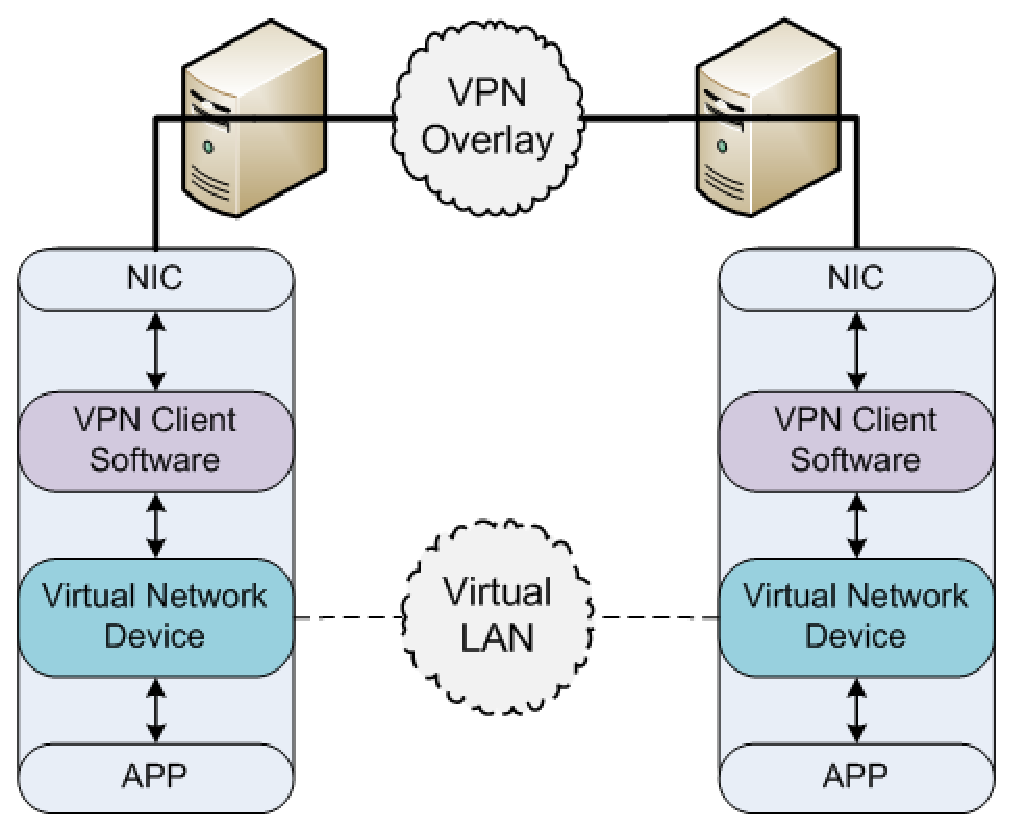
\epsfig{file=figs/vpn.png.eps, width=4in}

\caption[A typical VPN client]{A typical VPN client.  A VN device makes
application interaction with the VPN transparent.  Packets going to the VPN
destination are sent by routing rules to the VN device interfaced by the VPN
client.  The VPN client sends and receives packets from other VPN participants
via the hosts physical network device.}

\label{fig:vpn}
\end{figure}

Figure~\ref{fig:vpn} abstracts the common features of all VPNs clients, a
service and a virtual network (VN) device providing communication with the VPN
system and host integration, respectively.  During initialization, the VPN
service authenticates with the overlay by means of a centralized or distributed
service, indepently with each peer, or some other means; then, optionally,
querying for information about the network, such as network address space,
address allocations, and domain name service (DNS) servers.  At which point,
the VPN enables secure communication amongst participants.

Clients can authenticate with the overlay using a variety of methods.  A system
can be setup quickly by using null (no) authentication or a shared secret such
as a key or a password.  Using accounts and passwords with or without a shared
secret provides individualized authentication, allowing an administrator to
block all users if the shared secret is compromised or individual users who act
maliciously.  Using unique private keys with corresponding signed certificates
provide a more secure approach, because it eliminates the feasibility of brute
force attacks.  The trade-offs in the approaches come in terms of security,
usability, and management.  While the use of signed certificates provides
better security than shared secrets, certificates require more configuration
and maintenance.  In a system comprising of non-experts, like many university
VPNs, the usual setup uses a shared secret and individual user accounts.
Secrets can be packaged with the VPN application, so long as it is distributed
through secure channels such as authenticated HTTPS.

A VN device allows networking applications to communicate transparently over
the VPN.  The VN device provides mechanisms for injecting incoming packets into
and retrieving outgoing packets from the networking stack, enabling the use of
common network APIs such as Berkeley Sockets, allowing existing applications to
work over the VPN without modification.  While there are many different types
of VN devices, TAP~\cite{tap} stands out from the rest due to its open source
and pervasive nature.  TAP allows the creation of one or more Virtual Ethernet
and / or IP devices and is available for almost all modern operating systems
including Windows, Linux, Mac OS/X, BSD, and Solaris.  A TAP device presents
itself as a character device providing read and write operations.  Incoming
packets from the VPN are written to the TAP device and the networking stack in
the OS delivers the packet to the appropriate socket.  Outgoing packets from
local sockets are read from the TAP device.

VN devices are no different than any other network device.  They can be
configured manually through command-line tools or OS' APIs or dynamically by
the universally supported dynamic host configuration process
(DHCP)~\cite{dhcp0, dhcp1}.  Upon the VN device obtaining an IP address, the
system adds a new rule to the routing table that directs all packets sent to
the VPN address space to be directed to the VN device.  Packets read from the
TAP device are encrypted and sent to the overlay via the VPN client.  The
overlay delivers the packet to another client or a server with a VN stack
enabled.  Received packets are decrypted, verified for authenticity, and then
written to the VN device.  In most cases, the IP layer header remains
unchanged, while VPN configuration determines how the Ethernet header is
handled.

\section{Computer Network Architectures}

All models for computer communication in distributed systems fall under two
categories:  centralized and decentralized.  Sub-classes of these categories
include hybrid systems with centralized session management and decentralized
communication and self-configuring, dynamic P2P systems.  The architectures
commonly used for implementing VPN systems are centralized organization and
communication, centralized organization and decentralized communication,
decentralized communication with manual organization, and decentralized
communication with automatic organization.

Systems with Centralized organization and communication consist of clients and
servers where all distributed peers are clients discovering and connecting, or
organizing, through a dedicated centralized resource. Clients never communicate
with each other directly, but rather every message between two clients must
traverse the server.  For instance, most online social networks (OSNs) are
representative of these type of systems.  Users of OSNs like
Facebook~\cite{facebook} and MySpace~\cite{myspace} communicate through
centralized environments, never directly to each other's computers.
OpenVPN~\cite{openvpn} represents this VPN approach.  These systems rely on
dedicated resources.  In the situation that a server goes offline or becomes
overwhelmed by the clients, the system is rendered useless.

Centralized organization and decentralized communication systems include the
first set of popular P2P systems, such as the original Napster, Kazaa, and VPNs
like Hamachi~\cite{hamachi}.  Similar to the client-server model, clients
connect to a server to find other clients, though instead of communicating
through the server, the clients form direct connections with each other.  These
approaches are limited by network address translation (NAT) and firewalls that
may prevent peers from communicating with each other.  In these cases, the
central server may act as a relay allowing the two clients to communicate
through it.  Unlike systems using centralized communication, these systems are
less susceptible to being overwhelmed by client traffic and even if the server
goes offline existing client links remain active, though new connections cannot
be established.

Systems employing decentralized communication with manual organization address
the issues of a central system going offline, because clients are configured to
connect to any number of distributed servers forming an overlay.  In these
systems, servers are explicitly configured to communicate with other servers.
Though this approach improves upon the performance and availability issues
inherent to completely centralized architectures, if a server goes offline any
systems communicating through it will no longer be connected to the rest of the
system until the administrator creates additional links or the server becomes
active again.  Clients in these systems do not typically form direct links with
each other; rather, they route packets through the overlay.  This approach has
been used to create scalable VPNs, like ViNe~\cite{vine}, VNET~\cite{vnet},
Violin~\cite{violin}, and Layer 2 Tunneling Protocol based VPNs~\cite{l2tp}.

In automatic organization-based decentralized communication systems, there is
no distinction amongst peers as they act as both client and servers, i.e., a
P2P system or overlay.  P2P systems are usually distributed with a list of
common peers.  A peer attempting to bootstrap into the P2P overlay randomly
selects peers on this list until it is able to connect with one.  This
connection is then used to form connections with other peers currently in the
overlay.  The overlay can be organized in two different forms: randomly or
deterministically creating unstructured or structured overlays, respectively.
In an unstructured overlay, links are formed arbitrarily, thus a peer searches
for another peer by broadcasting the message or using stochastic techniques.
In structured overlays, peers organize into topologies by deterministically
forming connections with peers nearby in the overlay address space creating
structures such as ring and hybercubes.  Peers can be found deterministically
using greedy routing approaches in usually $\log(N)$ time.
Gnutella~\cite{gnutella} file sharing system and Skype~\cite{skype} are popular
examples of unstructured systems, while P2PSIP~\cite{p2psip} and distributed
hash tables (DHTs)~\cite{chord} are popular in structured systems.  A challenge
in unstructured systems is finding data objects in reasonable amount of time,
while structured systems suffer when large amount of peers join or leave the
system, known as churn~\cite{opendht}.  In general, both approaches are
difficult to secure depending on the nature of the application and deployment.
When used in private environments though, they have been shown to be very
useful, exemplified by Dynamo~\cite{dynamo} or BigTable~\cite{bigtable}.

This dissertation uses structured overlays as the foundation in building
scalable, decentralized VPNs, the following section reviews structured
overlays.

\section{Structured Overlays}

Structured P2P overlays provide distributed querying systems with guaranteed
search time.  Unlike unstructured systems~\cite{unstructured_v_structured},
which rely on global knowledge/broadcast or stochastic techniques such as
random walks that take $O(N)$ time to guarantee finding data in the overlay,
structured overlays organize into well-defined geometries with support to
resolve queries within $O(\log(N))$ There exists a plethora of structured
systems found both in research and in available applications~\cite{pastry,
chord, symphony, kademlia, can, brunet}.  In order to obtain guaranteed search
time, structured systems self-organizing into well defined topologies, such as
a ring (pictured in Figure~\ref{fig:ring_overlay}) or a hypercube.  Peers
joining an overlay typically follow these abstracted steps:

\begin{figure}
\centering
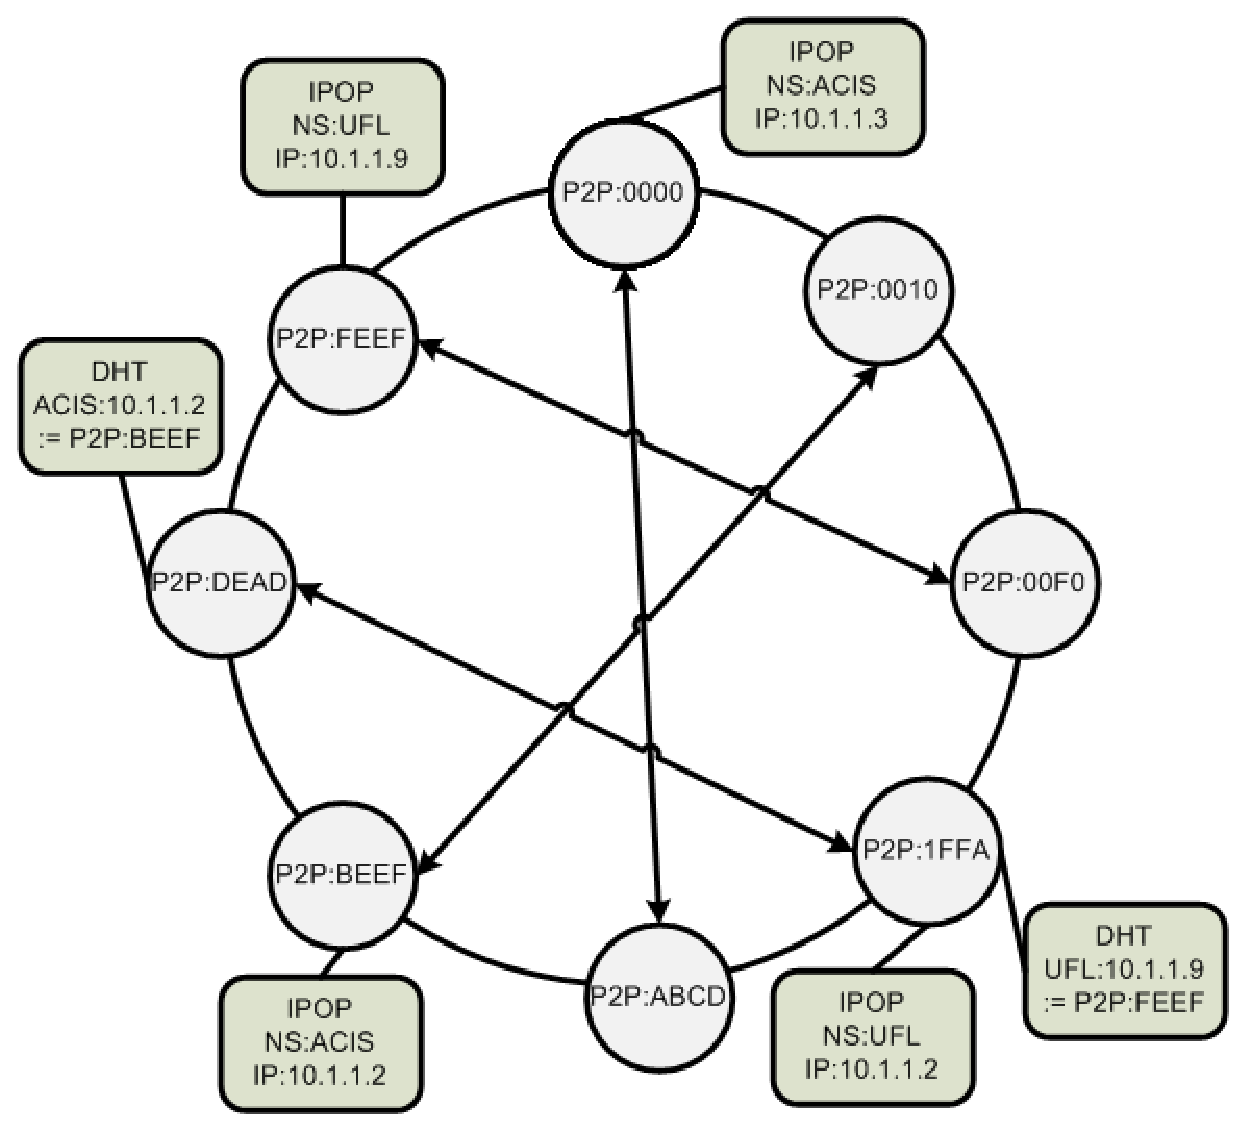
\epsfig{file=figs/ring.eps, width=6in}
\caption{1-D ring structured overlay}
\label{fig:ring_overlay}
\end{figure}

\begin{enumerate}

\item generate or obtain a unique identification number (node ID) within the
overlay's address space, usually on the order of 128-bits to 256-bits;

\item attempt to connect to one or more random addresses from a pre-shared list
of well-known endpoints, dedicates resources from a service provider or users
with high uptime;

\item become connected to at least one peer in this list (leaf connection,
bootstrap peer);

\item find the set of peers in the address space closest to the node's ID;

\item establish connections or exchange connection information with those peers
(neighbor or near connections);

\item and finally connect to other nodes in the overlay outside the set of near
connections to enable quickly traversing the address space (shortcut or far
connections).

\end{enumerate}

All nodes are required to have a unique node ID.  Address collisions can cause
inconsistencies in the overlay, where one or both of the nodes will not be
able to properly connect to the overlay.  Furthermore, having uniformly
distributed node IDs enhances the utility of the shortcut connections.  To
obtain a good distribution of node IDs, either a central server can provide
the ID or each node independently of others can use a cryptographically strong
random number generator.  The former approach can be used to create a trusted
overlay by having the third-party sign each node IDs~\cite{secure_routing}.

In a ring, each node must be connected to closest neighbors in the node ID
address space, that is the node immediately before and after it.
Optimizations for fault tolerance suggest that for ring topologies the amount
should be at least 2 and up to $\log(N)$ on both sides.  Consider the case
when there is overlay disconnectivity potentially due to churn; a peer
receives a packet but cannot route it closer to the destination than itself
because it does not have a connection with that peer.  The message may either
be locally consumed or thrown away never arriving at its intended destination.
Increasing the number of near neighbor peers reduces the likelihood chances of
packets being lost due to churn, especially if peers leave suddenly without
warning.

As mentioned, shortcuts or far connections enable efficient routing in
ring-based and similarly designed structured overlays.  The various shortcut
selection methods include: maintaining large tables without using connections
and only verifying usability when routing messages~\cite{pastry, kademlia},
maintaining a connection with a peer at specific locations in the P2P address
space~\cite{chord}, or using locations drawn from a harmonic distribution in
the node address space~\cite{symphony}.

Structured overlays support decentralized query systems that can be used to
build distributed data structures such as a distributed hash table (DHT) by
mapping keys via a hash function to P2P IDs in an overlay.  The data associated
with the key is then stored at the node closest to the P2P id of the key and
for fault tolerance can be stored by other nodes nearby or more keys can be
generated by recursively hashing the original key.  Using the DHT primitives,
Past~\cite{past} and Kosha~\cite{kosha} projects have designed more complex
distributed data stores.

The actual mechanism for querying nodes or routing in a P2P overlay can be
either iterative or recursive.  In iterative routing, the querying node
iteratively contacts nodes closer and closer to the address until finding the
closest node at which point it makes the request directly to that node.  In
more detail, the querying node directly queries the node closest to the
destination, that node returns back one or more network (IP) and P2P addresses
of closer peers, the querying node queries these peers, and the process
continues until determining there exists no closer node.  Alternatively in
recursive routing, a querying peer sends the message to the peer closest to
the destination from its perspective, repeating the process until the message
has arrived at the closest peer to the address or the destination.  Compared
to recursive routing, iterative can be implement more easily though with
considerable overhead as each overlay query will cause $\log(N)$ connections
to form.  NATs further complicate the use of iterative routing as peers
attempting to connect with another peer behind a NAT will need the assistance
of a third-party, whereas recursive routing maintains active connections and
messages, seamlessly traversing NAT links and non-NAT links since the
connections are established prior to message transmission.

\section{Network Asymmetries}

Naive P2P systems assume network symmetry, that is any peer can communicate
directly with any other peer using the underlying infrastructure.  Unless the
software is run inside a LAN or an environment where the network topology is
well controlled and defined, symmetry cannot be guaranteed.  P2P used in wide
area systems often relies on the Internet.  Besides the potential routing
outages on the Internet, significant amount of resources which are not directly
accessibe are connected to it.  The issue is only further pressed by the
current means of connecting to the Internet: Internet Protocol (IP) version 4
(IPv4) with its limited address space of only $2^{32}$ (approximately 4
billion).  With the Earth's population at over 6.8 billion and each individual
potentially having multiple Internet-capable devices, these limitations become
more apparent.

Currently the two approaches addressing IPv4 limitations are:  the use of
NATs to enable many machines and devices to share a single IP address but
preventing bidirectional connection initiation and IPv6 which supports
$2^{128}$ addresses.  The use of NATs, as shown in Figure~\ref{fig:nat},
complicates the bootstrapping of P2P systems as it prevents peers from simply
exchanging addresses with each other to form connections, as the addresses may
not be public.  In addition, firewalls may prevent peers from receiving
incoming connections.  Thus, while the eventual widespread use IPv6 may
eliminate the need for address translation, it does not deal with the issue of
firewalls preventing P2P applications from communicating as well as routing
outages, and it is not clear that IPv6 users will not continue to rely on
NAT/firewall devices to provide a well-defined boundary of isolation for their
local networks.

\begin{figure}
\centering
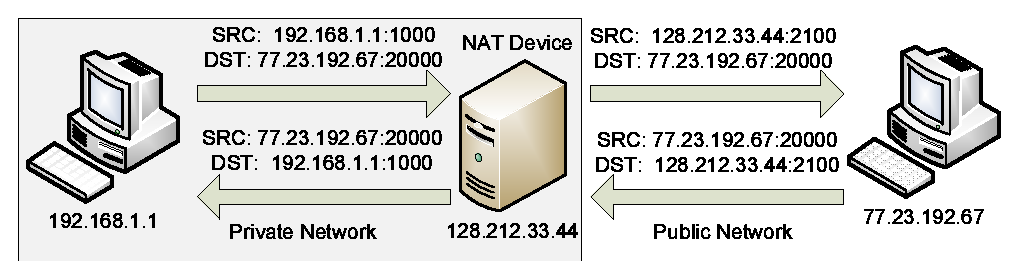
\epsfig{file=figs/NAT.eps, width=5in}
\caption[A typical NAT interaction]{A typical NAT interaction. The peer behind
a NAT has a private address.  When the packet is sent through the NAT, the NAT
translates the source information into a public mapping, keeping the original
source information so that if a packet from the remote peer comes back, it can
be translated and delivered to the original source.}
\label{fig:nat}
\end{figure}

When a machine, \textit{A}, behind a typical NAT, \textit{B}, sends out a
packet to an Internet host, \textit{C}, the NAT device translates the packet so
that it appears it is coming from the NAT device making the NAT device a
gateway.  When the packet is sent from \textit{A} to \textit{C}, the source and
destination are listed as $IP:port$ pairs, where the source and destination are
$IP_A:Port_A$ and $IP_C:Port_C$, respectively.  \textit{A} forwards the packet
to \textit{B} who transforms the source from $IP_A:Port_A$ to $IP_B:Port_B$,
where $Port_A$ may or may not be equal to $Port_B$.  This creates a NAT mapping
so that incoming packets from $IP_C:Port_C$ to $IP_B:Port_B$ are translated and
forwarded to $IP_A:Port_A$.

There are a handful of recognized NAT devices as presented in~\cite{stun,
p2p_nats_rfc}.  The following list focuses on the more prevalent types:

\begin{itemize}

\item FULL CONE. All requests from the same internal IP and port are mapped to
a static external IP and port, thus any external host can communicate with the
internal host once a mapping has been made.

\item RESTRICTED CONE. Like a full cone, but it requires that the internal host
has sent a message to the external host before the NAT will pass the packets.

\item PORT RESTRICTED CONE. Like a restricted cone, but it requires that the
internal host has sent the packet to the external hosts specific port, before
the NAT will pass packets.

\item SYMMETRIC. Each source and destination pair have no relation, thus only a
machine receiving a message from an internal host can send a message back.

\end{itemize}

Of the various scenarios involving peers and NATs, so long as one peer is on
any of the cone NATs and there are no firewalls, it can receive incoming
connection requests.  Challenges to this approach exist when firewalls are
introduced or both peers are behind symmetric NATs.  Firewalls may traffic that
would otherwise allow NAT traversal, whereas symmetric NATs require complex
mechanisms in an attempt to have incoming connection requests.  These types of
systems typically rely on a third-party to pass messages between the peers.

\section{Contributions}

The resulting expectations of a collaborative environment that addresses the
challenges listed in the introduction are self-configuring environments
enabling even non-experts to setup, deploy, and manage their own VPNs; peers
should communicate with each other directly when possible or through efficient
indirect paths when constrained; and the system should be reliable and ensure
the privacy of its users To address these requirements, I propose a novel
GroupVPN using structured overlays consisting of the following novel
contributions:

SECURE OVERLAYS. Typical overlays are secured using heuristics that limit the
effects of malicious users.  Challenges of using secure sessions for
instituting trust or security into an overlay depends on the communication
path ways.  If the goal for the system is to support asymmetries on the
network, then the system will have to make significant use of datagram
technologies.  This work proposes a unique filter mechanism to support
encrypting any form of communication between two parties and examines the
overheads of deploying it in simulated and real environments.

BOOTSTRAPPING AD-HOC, DECENTRALIZED SYSTEMS. Secure overlays present a
challenge when there is a one to one mapping between overlay and VPN in order
to securely isolate a VPN.  This stems from the fact that at any given time,
peers may or may not be connected to the overlay.  When used in small groups,
most or all members may be behind NATs or remain online for short periods of
time, creating a situation where not a single user on a publicly addressable
resource will be online, limiting the use of private overlays.  To address
this issue, I propose the reusing of public free-to-join overlays to bootstrap
into a private overlay.  Peers use the public overlay to find each other and
exchange connection information using secure messages.  Only peers with
appropriate security credentials are able to join the private overlay.

DECENTRALIZED RELAYS. In collaborative environments, most peers are behind NATs
and potentially firewalls as well.  While in general most NATs are traversable
through existing approaches, not all are.  Firewalls only complicate the
matter.  While these peers may be able to communicate through the overlay, as
the overlay grows, this latency can become a hindrace to usability and
interactivity.  To improve this situation, I propose the creation of autonomic
2-hop relays between the peers.

USING SOCIAL INFRASTRUCTURES FOR MANAGEMENT AND DISTRIBUTION OF SECURITY
CREDENTIALS. In order to simplify the management and access to a VPN, this
component explores the use of social networks in terms of both groups and
peers to facilitate trust establishment for a VPN.  Beyond the contribution of
uniquely using social networks to establish VPN trust, this work shows how
systems can leverage trust in an existing environments for use in another.

SELF-CONFIGURING VPN ARCHITECTURES. Many existing VPN approaches require the
users to setup their environment and do not provide a plug and play system.  In
addition, different environments call for different types of VPNs, explicitly,
individual users connect via their own VPN connections, while clusters may
benefit from a shared VPN or may desire fault tolerance of having many but do
not want the communication overhead when talking to VPN peers on the LAN.  I
address this issue with a self-configuring VPN approach that can be applied to
various local environments scaling from a single computer to many.

P2P VPN ENABLED INTERNET TRAFFIC TUNNELING. When in insecure environments such
as browsing private information in a coffee shop, users may desire to prevent
local users and administrators from sniffing their traffic.  Traditional VPNs
support this behavior, but the approach is difficult to implement in P2P
systems due to their dynamic nature.  Currently, no decentralized VPN supports
the ability to perform this behavior.  I propose a method that not only works
for decentralized and P2P systems but ensures a greater level of security than
existing approaches by securing other non-VPN communication between the peer
and gateway resources.

APPLICATIONS IN AD-HOC, DISTRIBUTED SYSTEMS. The value in a complex system
like the one proposed herein can be realized when tied together for the
creation of ad-hoc, distributed systems.  The type of system focused on in
this dissertation is a grid.  While there are many grid topologies, approaches
that share resources amongst users and even most that are used by a single
user require a user with expertise in operating systems, networks, and
middleware.  This dissertation shows the applicability of P2P VPN methods and
techniques that can be used to create a trusted, ad-hoc, distributed grid that
requires little if any expertise in the underlying technology being utilized.

DECENTRALIZED SOCIAL NETWORKS. Traditional approaches to social networks, such
as Facebook and MySpace, requires trust in a third-party entity.  These
third-parties mine users information for advertisements, potentially violating
user's privacy.  This dissertation presents a decentralized social network that
addresses real problems by taking advantage of the P2P system described herein
by providing each user in a social network their own private overlay whose
members constitute the friends of that individual.

IMPROVED MODELS FOR DIRECT CONNECTION ESTABLISHMENT.  Originally, direct links
in the P2P VN were based upon packet flow passing a threshold.  Through the use
of profiling real systems and published results of Internet behavior, I have
concluded that this model does not scale well and have design and implemented a
model that satisfactorily solves this problem.

The rest of this dissertation is organized as follows.
Chapter~\ref{chap:vpns} overviews existing VN and VPN approaches and discusses
configuration and organization of the VPN including end-point configuration.
In Chapter~\ref{chap:bootstrapping}, I review the challenges to bootstrapping
overlays and present my solution that reuses existing overlays to bootstrap
smaller, ad-hoc overlays.  This leads into Chapter~\ref{chap:security}, which
discusses security issues in structured overlays and addresses the means to
boot private and secure VPNs.  Chapter~\ref{chap:extensions} covers extensions
to the VPN based upon practical demands and experiences.
Chapters~\ref{chap:gridappliance} describes the Grid Appliance, the target
application for my research.  Chapter~\ref{chap:spo} presents a proposed idea
on how to use the technology discussed thus far to create a decentralized
online social network.  Finally, I conclude in Chapter~\ref{chap:conclusion}
by discussing the value in my contributions and challenges that were revealed
but not addressed in this body of work, thus motivating future work.

\chapter{VIRTUAL NETWORK CONFIGURATION AND ORGANIZATION}
\label{chap:vpns}

VPNs enable seamless communication in distributed computing particularly when
combinging large sets of remote resources or connecting to centralized or
personel resources.  Similar use cases can be extrapolated onto other
collaborative environments such as multiplayer games, merging home networks
over a VPN, or accessing a work computer remotely.  Each application has
different requirements and in review of related research~\cite{ipop, vine,
violin, vnet, ocala, softudc, openvpn, hamachi, wippien, gbridge, pvc, tinc,
n2n, p2pvpn, l2tp} not a single approach efficiently supports these dynamic
environments.  Certainly, ISP large scale VPNs such as Multiprotocol Label
Switching~\cite{mpls} (MPLS) do not as well due to the manual configuration and
expertise required.  An overview of these and the one described herein are
presented in Table~\ref{tab:virtual_networks}

The organization of a VPN has a direct effect on the amount of user effort
required to connect multiple sites.  In this regard there are two components of
a VPN, the local organization and the remote or network organization.  The
setup of the virtual network in order to have be a destination and recognized
source for remote packets constitute the local organization, whereas the
routing of the packets amongst peers is handled by the network organization.
Prior research works primarily focused on the latter issue, while ignoring the
former.  This left users to setup their own address allocations either through
manually configuring each environment or dealing with the problems caused by
DHCP servers in cross domain network construction, as well as their own
security distribution systems.  In addition, organizing a network can be an
even more complicated task than locally configuring the network, because it may
require the cooperation of many administrators at the various sites.  This
chapter presents a novel approach to VPNs that achieves both local and network
self-configuration.

\section{Network Configuration} The key to communicating in a VPN is creating
links to the VPN and finding the peer in the VPN.  The different architectures
for VPN link creation are based on the methods described in
Table~\ref{tab:vpn_types}.  These approaches are described in more detail
below.

\begin{center}
\begin{table}
\caption{VPN Network Classifications}
\label{tab:vpn_types}
\begin{tabular}{p{1.5in}p{4.5in}} \hline
Type & Description \\ \hline \hline
Centralized & Clients communicate through one or more servers which are statically
configured \\ \hline
Centralized Servers / P2P Clients & Servers provide authentication, session management, and
optionally relay traffic; peers may communicate directly with each
other via P2P links if NAT traversal succeeds\\ \hline
Decentralized Servers and Clients & No distinction between clients and servers;
each member in the system authenticates directly with each other; links between
members must be explicitly defined \\ \hline
Unstructured P2P & No distinction between clients and servers; members either know
the entire network or use broadcast to discover routes between each other \\ \hline
Structured P2P & No distinction between clients and servers; members are usually
within $O(\log N)$ hops of each other via a greedy routing algorithm; use
distributed data store for discovery \\ \hline
\end{tabular}
\end{table}
\end{center}


\subsection{Centralized VPN Systems}

OpenVPN is an open and well-documented platform for deploying centralized VPNs.
In this dissertation, it is used as the basis for understanding centralized
VPNs as it represents features common to most centralized VPNs.

In centralized VPN systems, clients forward all VPN related packets to the
server.  Client responsibilities are limited to configuring the VN device and
authenticating with the VPN server, whereas the servers are responsible for
authentication and routing between clients and providing access to the servers'
local resources and the Internet (full tunnel).  Likewise, broadcast and
multicast packets also must pass through the central server.

Centralized VPNs can support multiple servers: upon starting, the client can
randomly select from a list of known servers, implementing a simple load
balance.  Once connected, the servers provide the client an IP address in the
VPN address space. Depending on configuration, this allows a client to
communicate with other clients, resources on the server's network, or Internet
hosts via the VPN.  Servers require additional configuration to communicate
with each other.

All inter-client communication flows through a central server.  By default, a
client encrypts a packet and sends it to the server.  Upon receiving the
packet, the server decrypts it, determines where to relay it, encrypts it, and
then sends the packet to its destination.  This model allows a server to
eavesdrop on communication.  While a second layer of encryption is possible
through a shared secret, it requires out-of-band communication and increases
the computing overhead on communication.


\subsection{Centralized P2P VPN Systems}

Hamachi~\cite{hamachi} is the first well-known centralized VPN that used the
ambiguous moniker ``P2P VPN''.  In reality, these systems are better classified
as centralized VPN servers with P2P links.  Similar VPNs include
Wippien~\cite{wippien}, Gbridge~\cite{gbridge}, PVC~\cite{pvc}, and
P2PVPN\footnote{Due to the similarities between the name P2PVPN and focus of
this dissertation, ``P2PVPN'' refers to ~\cite{p2pvpn} and ``P2P VPN'' to to
the use of P2P in VPNs.}~\cite{p2pvpn}.  The P2P in these systems is limited to
direct connectivity between clients orchestrated through a central server: in
Wippien it is a chat server, while P2PVPN uses a BitTorrent tracker.  If NAT
traversal or firewalls prevent direct connectivity, the central server can act
as a relay.  Each approach uses their own security protocols with most using a
server to verify the authenticity and setup secure connections between clients.
In regards to the P2PVPN, long term goals involve the creation of an
unstructured, which would provide a method of decentralized organization.

\subsection{Decentralized VPN Systems}
Some examples of systems that assist in distributing load in VPN systems are
tinc~\cite{tinc}, CloudVPN~\cite{cloudvpn}, ViNe~\cite{vine}, VNET~\cite{vnet},
and Violin~\cite{violin}.  These systems are not autonomic and require explicit
specification of links between resources.  This means that, like OpenVPN, these
systems can suffer VPN outages when nodes go offline, thus administrators must
maintain the VPN connection table.  Unlike OpenVPN, these approaches typically
do not require all-to-all direct connectivity for all-to-all communication.
Users can either setup out-of-band NAT traversal or route through relays.  Links
are manually configured.

\subsection{Unstructured P2P VPN Systems} Unlike centralized and decentralized
systems, P2P environments require the user to connect to the overlay, which
then automatically configures links.  The simplest form of overlays are
unstructured, where peers form random connections with each other and use
broadcast and stochastic (e.g. random walks) techniques to find information and
other peers; however, due to its unstructured nature, the system cannot
guarantee distance and routability between peers.  The only example of an
unstructured VPN is N2N~\cite{n2n}.  In N2N, peers first connect to a super
node and then, to find another peer, they broadcast discovery messages to the
entire overlay.  In the case that peers cannot form direct connection, peers
can route to each other over the N2N overlay.  In the realm of VPNs, all client
VPNs are also servers performing authentication though neither approach deals
with decentralized address allocation.

\subsection{Structured P2P VPN Systems}

To address the scalability concerns in unstructured systems, this work uses
structured P2P overlays.  As described in the first chapter, structured P2P
overlays provide distributed look up services with guaranteed search time with
in $O(\log(N))$ time in contrast to unstructed systems with $O(N)$ time.  In
general, structured systems are able to make these guarantees by
self-organizing a structured topology, such as a 1-D ring or a hypercube,
deterministically by randomly generated node identifiers.

The primary feature used by structured overlays is a distributed data store
known as a distribute hash table (DHT), which stores key, value pairs.  In
the overlay, the key is an overlay address, where the value is stored.  The
peer closest to the key's overlay address is responsible for maintaining the
value.  Cryptographic hashes like SHA and MD5 can be used to obtain the key's
overlay address from a string or some other byte array.

In~\cite{pcgrid07, i3}, a method for address allocation is described by using
the DHT.  Each VPN has a unique name or namespace, when a peer requests an
IP address, a mapping of $hash(namespace, IP)$ to the peers overlay address
is atomically written to the DHT.  A success implies that the writer was the
first writer to that value and other peers reading that value will be able to
identify that peer as owner of that IP address in that namespace.  Likewise
when a peer wants to route a packet to a remote VPN peer, they query the DHT
using the mapping, which returns the overlay address.  The IP packet is then
sent to the overlay destination.

Unicast messages are sent between two end points on the overlay using normal
overlay routing mechanisms.  Direct overlay links can be used to improve
performance between end points.  ~\cite{ipop} describes a method by which peers
can form autonomic direct connections with each other using an unstructured
overlay.  As IP traffic increases over a period of time, a direct connection to
bypass the overlay is initiated by the receiver of the packets.  Alternatively,
a VPN may wish to form all-to-all connections with VPN peers as described
in~\cite{cops08}.

To support broadcast and multicast in an overlay, all members of a subnet
associate through the DHT by placing their overlay address at a specific key,
i.e., $namespace:broadcast$.  Then when such a packet is received, it is sent
to all addresses associated with that key.  It is up to the VN at each site to
filter the packet.  This is sufficient to support deployments where multicast
or broadcast is not relied upon extensively.  

\section{Local Configuration} At first order, there are two approaches to local
VPN configuration: a single VN endpoint per a host (Interface) and a VN router
endpoint for many hosts on the same LAN (Router).  The components differing
between the two approaches are:

\begin{itemize}

\item SOFTWARE LOCATION. Interfaces execute the software on each VPN connected
resource, whereas any machine connected to the same LAN as a Router will be
able to access the VPN.  The Router requires a dedicated resource.

\item NETWORK CONFIGURATION. Since the Interface software runs on each machine,
it is able to directly configure networking parameters, whereas a Router must
use external methods to configure the resources.

\item COMMUNICATION ON A LAN. When two peers on a LAN using a VPN Interface to
communicate, all traffic must pass through the VPN adding unnecessary overhead,
though in a Router the two peers have a merged physical and virtual network
between them and the traffic is able to bypass the VPN.

\item FAULT TOLERANCE. The Router only has a single instance running, when it
goes offline, all resources will lose their VPN access, whereas each individual
resource has their own Interface and is responsible for their own VPN
connectivity.

\item COMMUNICATION OVER THE WAN. Performing encryption can be expensive and
may limit the bandwidth available due to CPU constraints.  A Router may
struggle to use all the available bandwidth, whereas enough Interfaces will
eventually be able to use all the bandwidth.  Although each additional VPN
Interface also has idle traffic, potentially reducing usable bandwidth.

\end{itemize}

\begin{table}
\caption{Qualitative comparison of the three deployment models}
\label{tab:three_models}
\centering
\begin{tabular}{p{.95in}p{1.25in}p{1.5in}p{2.2in}} \hline
 & Interface & Router & Hybrid \\ \hline \hline
Host LAN 
& 
No assumption 
& 
Ideally, VLAN
&
No assumption, though may have duplicate address allocation in the same subnet
for different namespaces.\footnotemark[2]
\\ \hline
Host software
&
IPOP, tap
&
End node: none. Router: IPOP, tap, bridge 
&
IPOP, tap, VETH, bridge \\ \hline
Host overhead
&
CPU, memory
& 
End node: none. Router: CPU, memory
&
CPU, memory \\ \hline
LAN traffic
&
Through IPOP
&
\multicolumn{2}{c|}{Bypasses IPOP} \\ \hline
Migration
&
Handled by node
&
Involves source and target routers
&
Handled by node \\ \hline
Tolerance to faults
&
Nodes are independent
&
Router fault affects all LAN nodes
&
Nodes are independent \\ \hline
\end{tabular}
\end{table}

\begin{figure}
\centering
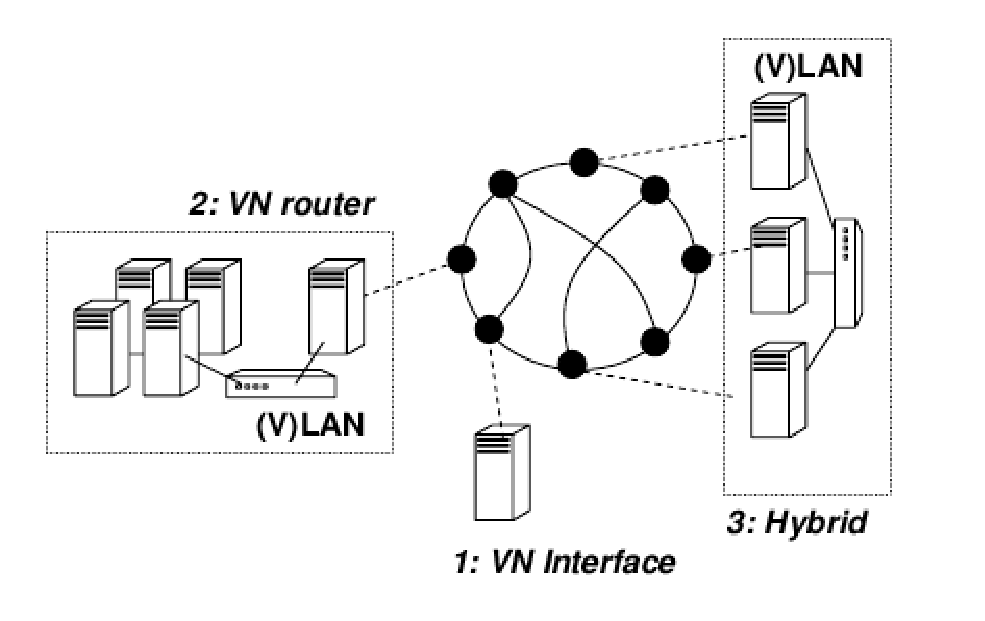
\epsfig{file=figs/three_models.png.eps}

\caption[Three VN Approaches]{Illustration of the three different deployment
models considered in this dissertation. In VN interface mode (1), each node has
an overlay ID and communicates to all other nodes through VN tunneling. In VN
router mode (2), only the router has an overlay ID and routes for a set of
resources; LAN communication does not require VN tunneling. In hybrid mode (3),
each host has an overlay ID; LAN communication does not require VN tunneling.}

\label{fig:three_models}
\end{figure}

This dissertation identifies methods by which a single software stack can be
implemented to support self-configuration and resource migration in a way that
is platform independent.  This method lends itself to a new architecture known
as Hybrid, allowing an instance to be run on each VPN resource but enabling
direct communication amongst peers on a LAN as described in~\cite{sc09}.  The
architectures are shown communicating via an overlay in
Figure~\ref{fig:three_models} and compared in Table~\ref{tab:three_models}.
The two aspects that need configuration in the local configuration beyond the
VPN architecture are address allocation, obtaining and setting an IP address on
a resource, and address resolution, determining where to route a VPN packet.
The keys to creating this environment involve the use of standard network
protocols implemented uniformly across operating systems, including DHCP
(dynamic host configuration protocol) and ARP (address resolution protocol).
Many applications make use of names instead of IP addresses to resolve peers,
as such a naming system, like DNS (domain name service) is almost as important
as address resolution and allocation.  A state machine representation of this
architecture is shown in Figure~\ref{fig:vn}.

\begin{figure}[ht]
\centering
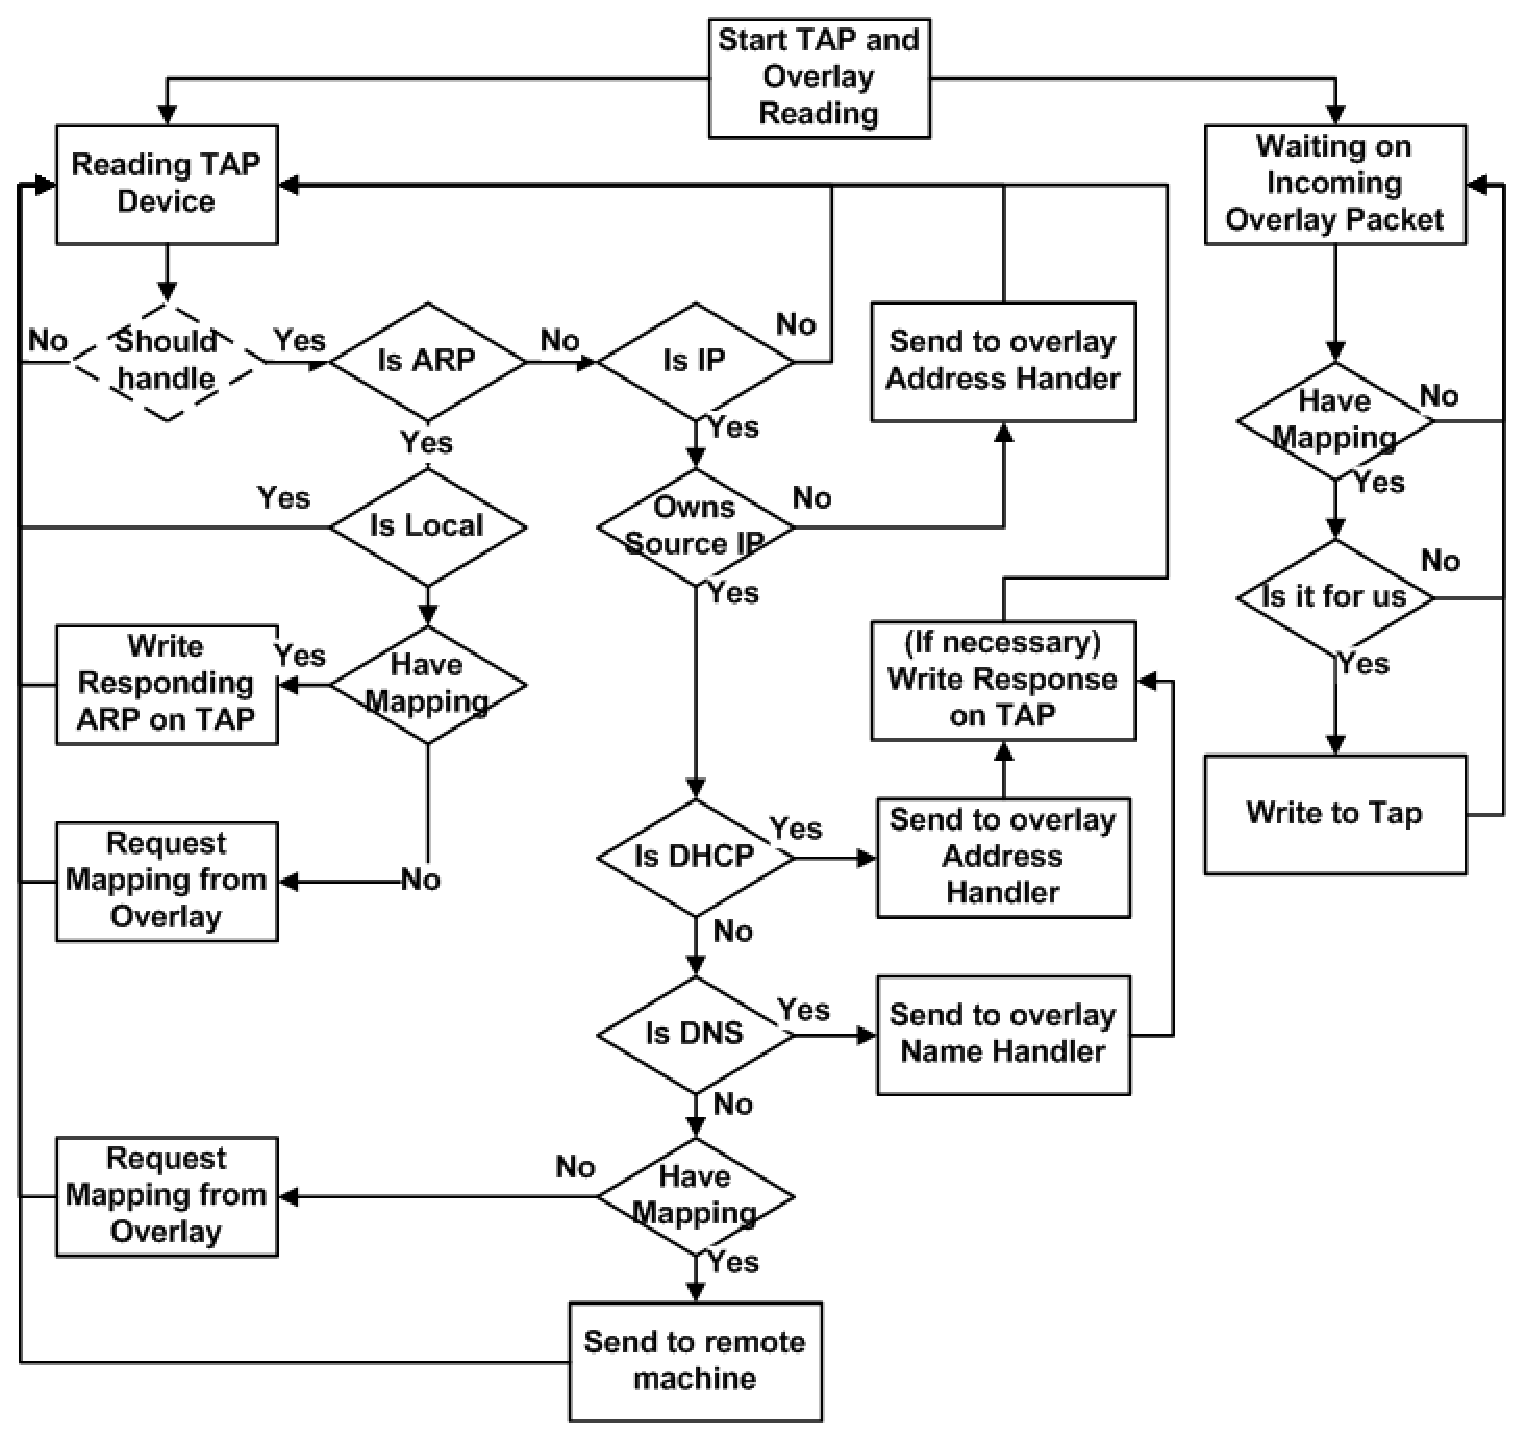
\epsfig{file=figs/vn.png.eps, width=\textwidth}
\caption[The state diagram of a self-configuring VN.]{The state diagram of a
self-configuring VN.  In this model, a VN interface is identical to a VN router
with the caveat that the TAP device is not bridged, thus isolating the VN
traffic.  The ``Should Handle'' with dashed lines is a feature that is specific
to the VN hybrid; that is, a VN hybrid must be configured to communicate for a
single network device.}
\label{fig:vn}
\end{figure}

\subsection{Local VPN Architecture}

\begin{figure}
\centering
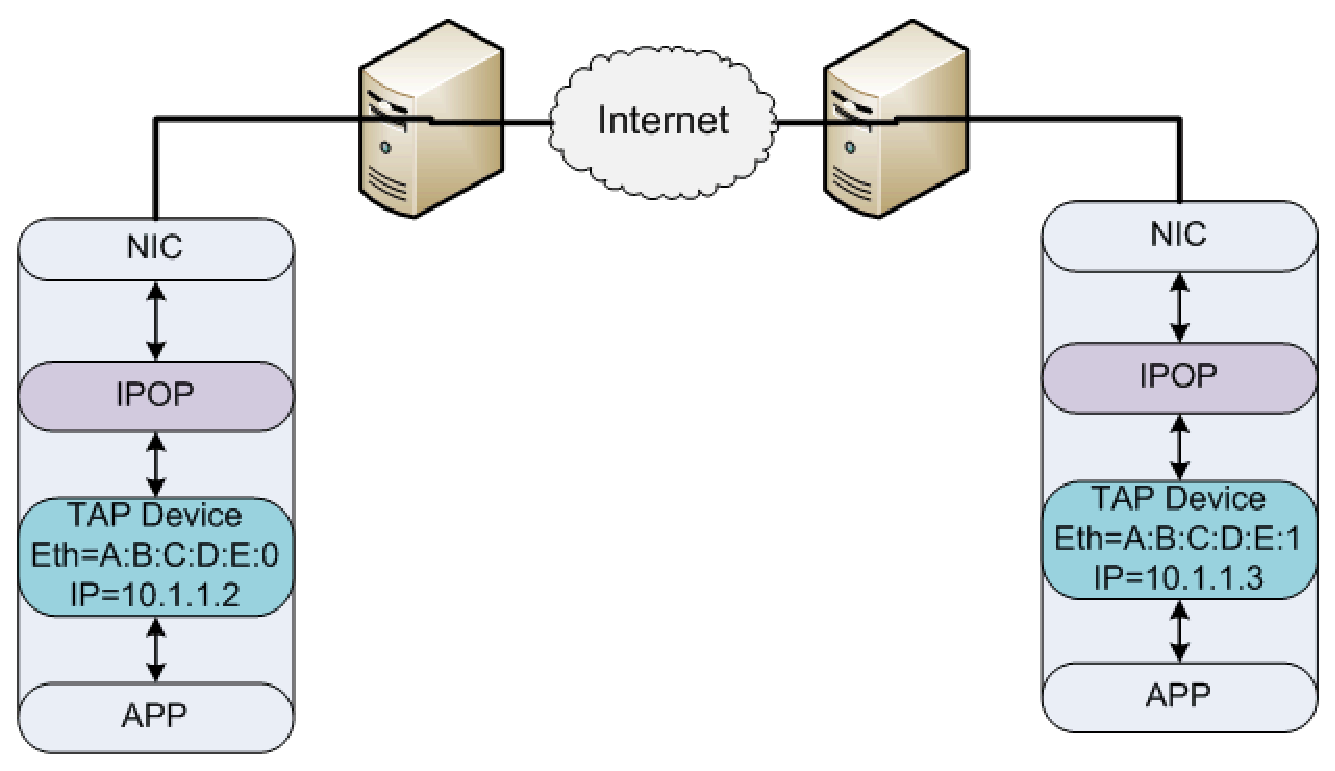
\epsfig{file=figs/tap_workstation.png.eps, width=\textwidth}
\caption[VN Interface]{A VN deployed as an interface for single machine usage.
The user of the machine is presented two interfaces on two different IP subnets.
All non-VN subnet based traffic is routed normally via the default interface.}
\label{fig:interface}
\end{figure}

As described in the introduction, the TAP device is the glue by which the local
resources communicate with the VPN.  Each approach relies on the TAP device
though in different configurations.  In the Interface
(Figure~\ref{fig:interface}), the TAP device is used directly by the user as
any other network device.  In short, packets are written to the TAP device by
the O/S sockets and read by the VPN software to send to the remote location,
packets received by the VPN are written to the TAP device and delivered to
sockets by the O/S.  The Router (Figure~\ref{fig:router}) bridges the TAP
device to a LAN, thus packets can be routed to it and sent through the VPN.
TAP device virtualizes a bridge to other physical networks.  

\begin{figure}
\centering
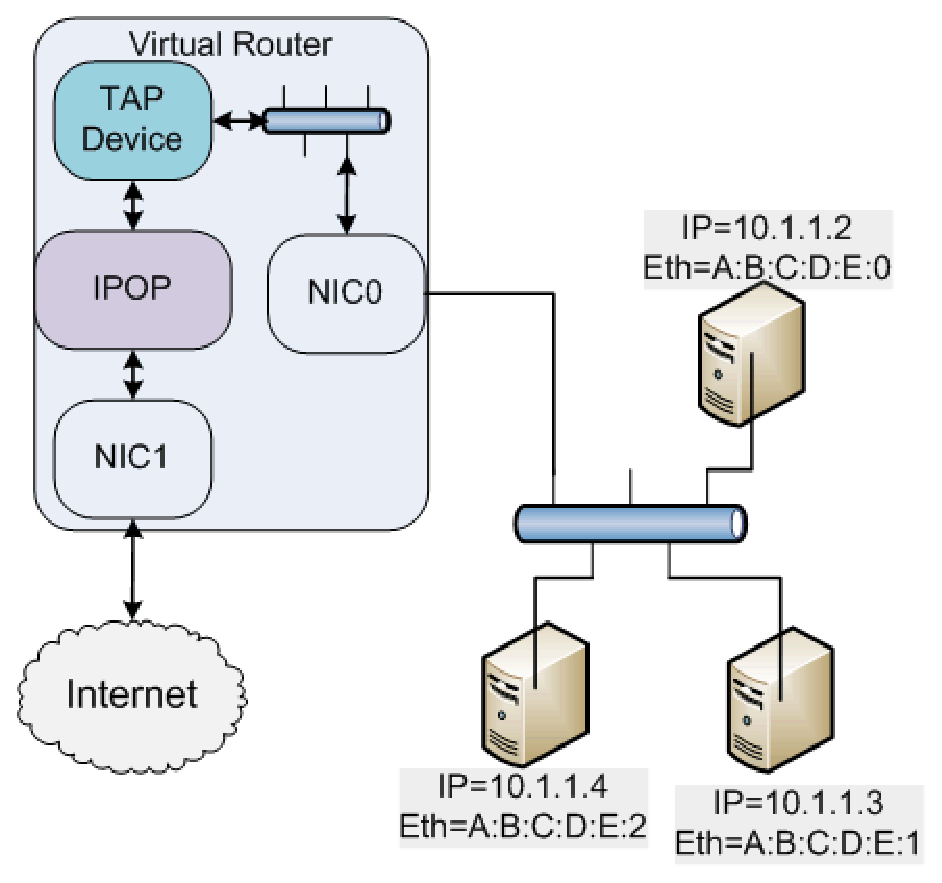
\epsfig{file=figs/tap_cluster.png.eps, width=4in}
\caption[VN Router]{A VN deployed as a router providing virtual network access
for an entire layer 2 network.  Each machine in the network only has a VN-based
address, though they can communicate directly with each other (and with proper
routing rules and NAT setup the Internet as well).  The machine hosting the VN
can also have an IP address in the network by assigning one to the bridge.}
\label{fig:router}
\end{figure}

Finally, the Hybrid (Figure~\ref{fig:hybrid}) like the Router connects to the
LAN but only allows configuration from the local host.  In Linux this is
possible through the use of a VETH pseudo device that provides a virtual
Ethernet pair, so that one end can be bridged with the TAP device and LAN while
the other provides another interface that can be configured on the LAN, which
will be used by the VPN.  The reason for this lies in the nature of the state
of the interfaces connected to the bridge, which go into promiscuous mode, so
that all packets sent to them are forwarded on as if they are on a wire as if
there were only a single network interface.  In non-promiscuous mode, the
network card will drop packets that are not destined for that network card.  So
in that case, it is not possible to assign more than one IP address to a
bridge, because it and all devices connected to it are viewed as one big
network interface.  Connecting the VETH device allows an additional uniquely
identifiable Ethernet addresses and thus additional IP addresses.  In contrast,
aliasing a Ethernet card only provide additional IP addresses and services that
rely on layer 2 networking. In this case, some services may not work, for
example, DHCP does not work on aliased network cards.

\begin{figure}
\centering
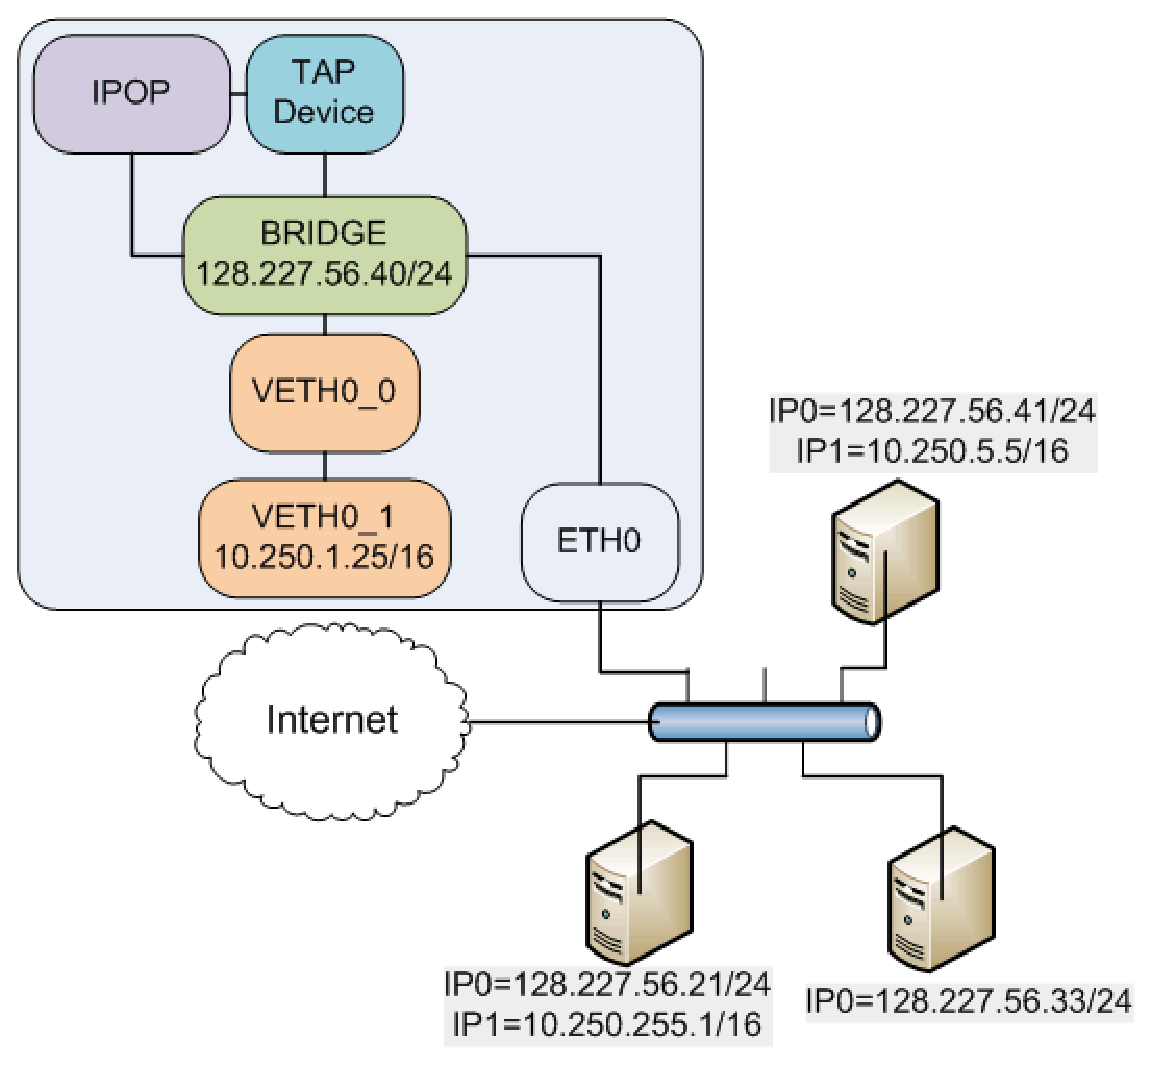
\epsfig{file=figs/tap_hybrid.png.eps, width=4in}
\caption[VN Hybrid]{A VN deployed in a hybrid mode providing virtual network
access for a single machine but bypassing the VN when a VN peer is local.  This
model is similar to having two network cards from a single machine going to one
switch.  The key feature is that this model allows a machine to be in multiple
IP address space subnets and have layer 2 traffic as well.}
\label{fig:hybrid}
\end{figure}

\subsection{Address Resolution}
\label{vpns:arp}

IP is a layer 3 protocol. Layer 2 devices such as switches, bridges, and hubs
are not aware of IP addresses.  When a system wants to send a layer 3 packet
over a layer 2 network, it first uses ARP to find the layer 2 address owning
the layer 3 address.  This process, as shown in Figure~\ref{fig:arp}, begins by
the sending of a layer 2 broadcast message which contains an ARP request,
asking all members in the LAN that the node owning the target IP address
respond to the sender of the request.  If a node owns the target IP address, it
responds with an ARP reply, making themselves the sender and the original
sender is the message recipient.  The Ethernet header consists of the source
address being the sender and the target being the destination.  By listening to
these requests, layer 2 devices such as a switch can autonomously learn the
location of nodes holding Ethernet addresses are and can forward packets
through appropriate ports as opposed to broadcasting or dropping them.

\begin{figure}
\centering
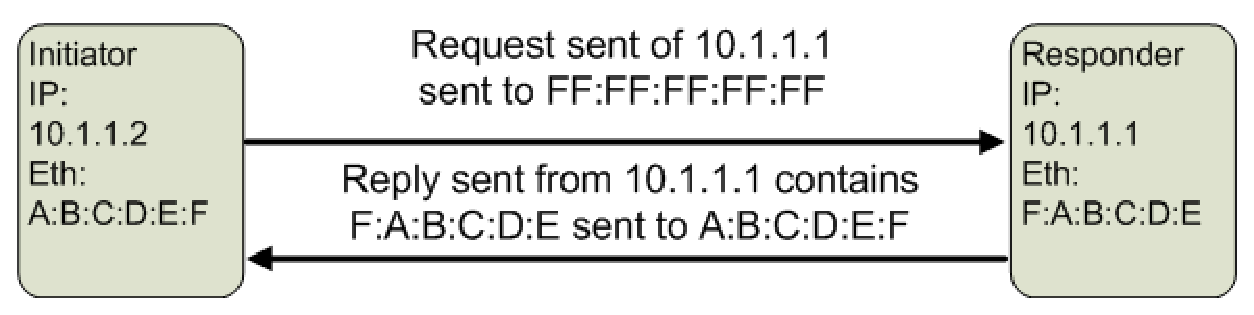
\epsfig{file=figs/arp.png.eps, width=4in}
\caption{ARP request/reply interaction}
\label{fig:arp}
\end{figure}

In a typical IP subnet, all machines talk directly with each other through
switches.  As such, they must learn each other's Ethernet address. The VN model
used herein focus on a large, flat subnet spanning across all nodes connected
to the VPN.  To accomplish this, the VN provides the ability to virtualize a
bridge, similar to proxy ARPs~\cite{RFC0925} used to implement a transparent
subnet gateway~\cite{RFC1027}.  In this scenario, the VN would need to respond
to the ARP packets with a fake layer 2 address.  Layer 2 devices in the system
would then route all packets destined for that layer 2 address to the VN.

As shown in the state machine (Figure~\ref{fig:vn}), ARPs are only responded to
if (a) they are inquiring about a VN IP address, (b) the VN address is not
locally allocated, and (c) there is a P2P:IP mapping.  If all those are true,
then an ARP response is sent back to the sender.  ARPs are occasionally sent
out during the course of communication and thus if a machine migrates to a VN
router, the VN router will no longer respond with ARPs.  An ARP response sent
by the VN requires a source Ethernet address, bridges and switches will see the
response and will forward all traffic towards the TAP device for that Ethernet
address.  A VN device can use the same Ethernet address for remote entities.

Prior to the introduction of the VN hybrid, the VNs used the Ethernet address
FE:FD:00:00:00:00 to refer to remote entities.  If each VN hybrid used this
address, there would be layer 2 collision causing a single hybrid to have all
traffic sent to it.  In hybrid mode, each VN must generate a unique ``remote''
Ethernet address at run time.  Experience and research has led to the
following solution: (1) use FE:FD for the first two bytes as they tend to be
unallocated and (2) assign random values to the 4 remaining bytes.   Applying
the birthday problem in this context, the expected probability of address
collisions is small for typical LAN environments (less than 50\% if the average
number of VN hybrid nodes on the same L2 network is 65,000). 

The key difference from the Hybrid and Router is that the Hybrid routes for only
a single node, say ``A'', and thus must ignore messages that do not originate
from ``A''.  The Hybrid model does not necessarily know about the existence of
all machines in a LAN, because it does not own them.  So when an ARP request
of some remote machine, say ``B'', is sent by ``A'', the Hybrid must send out
a matching request with the result being sent back to the pseudo-entity of the
transparent subnet gateway so that the VPN can determine if ``B'' exists
locally.  If no message is returned after a set amount of time (the reference
implementation used 2 seconds), then assuming that there is a peer in the
overlay with the IP address, the original ARP will be responded to with the
pseudo-entity being the target.

\subsection{Address Allocation}
IP addresses are traditionally allocated in one of three ways: 1) statically, 2)
dynamically through DHCP, or 3) through pseudo-random link-local addressing.
This model focuses on static and dynamic addressing.

\begin{figure}
\centering
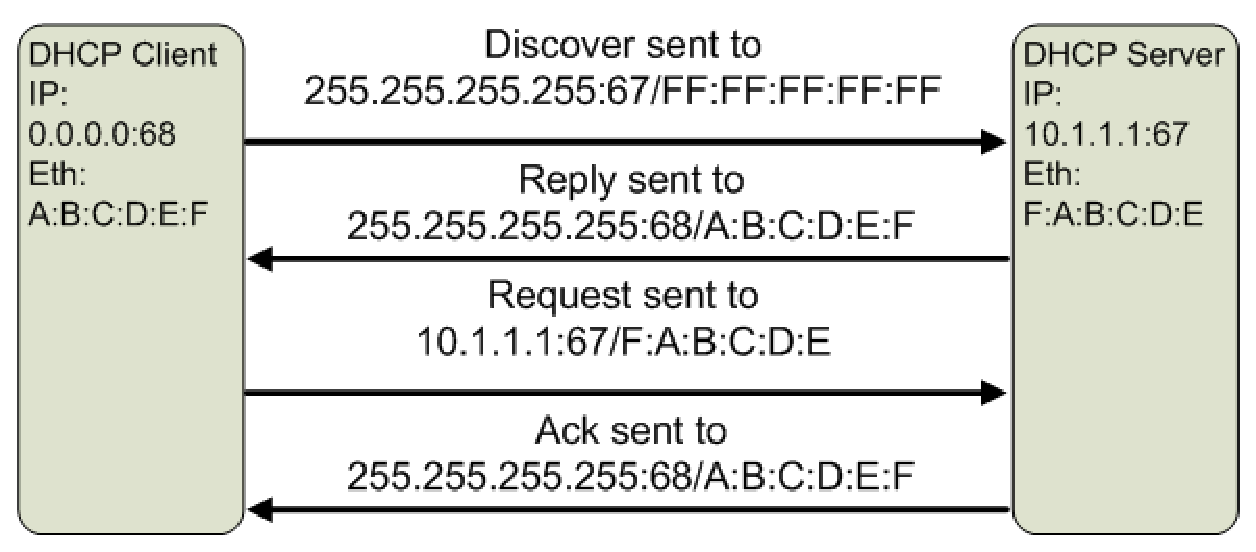
\epsfig{file=figs/dhcp.png.eps, width=4in}
\caption{DHCP client/server interaction}
\label{fig:dhcp}
\end{figure}

The network components configurable by DHCP as defined by~\cite{dhcp0,dhcp1}
that are interesting to a VPN are addresses, routing, and other networking
related features.  While many different client and servers exist, they all tend
to support the basic features of allowing the server to specify to a client and
IP address, a gateway address, and domain name servers.  As shown in
Figure~\ref{fig:dhcp}, the steps in DHCP are:

\begin{enumerate}

\item Client sends Discover packet requesting address.

\item Server receives the packet, allocates an address, and sends an Offer of
the address and other network configuration.

\item Client receives and acknowledges the Offer by sending a Request message
to accept the Offer.

\item Server receives Request message and returns an ACK message containing the
same details as the Offer.

\end{enumerate}

During the DHCP phase, the VPN communicates with a DHCP server for the VPN,
which will allocate an address for the requester.  Similarly, a VN model can
review packets coming into the VPN, review the sender IP address, and request
and notify the server of this allocation.  Treating static addresses like DHCP
enables easier configuration of the VPN, though it is difficult to handle
address conflicts.  In this model, this is done by the server ignoring the
duplicate requests, and it is up to the user to configure for a new address.
Thus DHCP provides a more reliable method in these systems.

To support scalable address allocation in decentralized systems, the
DHCP server is a virtual entity, parsing DHCP packets and interacting with
an overlay based DHT.  This approach does not need to be limited to structured
overlay based VPNs but can be introduced as an added value component.

An important aspect of DHCP is that after a machine has received an IP address
from the DHCP server, it always checks to ensure that the address has not been
allocated, as such the VPN should never respond to address resolutions for
local IP addresses.

If an overlay allocates an address to the VN, then the VN owns it.  The other
address that the VN owns is the null address, 0.0.0.0, which is sent during
DHCP to indicate that the machine has no address prior to the request.

\subsection{Domain Name Servers and Services}
Name services allow machines to be addressed with names that are more
meaningful to users than numeric addresses.  Certain applications and
services require domain name checking, such as Condor.  To support DNS, this
requires that the OS be programmed with the VN's DNS servers IP, typically
the lowest available IP address in a subnet.  In static configuration, this
process requires the user to manually add this address, though through DHCP
this is set automatically.

In the state representation of the VN (Figure~\ref{fig:vn}), the VN checks the
IP packet to ensure that the destination IP and port match that of the virtual
DNS server and the well-known DNS port, 53.  In the event of a match, the
packet is passed to the VN's handler for domain names.  Names are typically
used for the following purposes: 1) because applications require it, and 2) to
assist users in finding resources.  To deal with 1), the DNS can
deterministically maps IP addresses to names, such as 10.250.5.5 maps to
C250005005.  2) can be solved by using the DHT and placing key:value pairs of
the form hash(namespace:hostname) to IP address and hash(namespace:IP address)
to hostname.

\section{Supporting Migration}

There has been a rapid increase in the deployment of Virtual Machines (VMs) for
use in resource consolidation in the server industry as well as the domain of
cloud computing.  Providers of cloud computing services have adopted virtual
machines as the unit of granularity for providing services and service level
agreement to the users.  Users are billed according to the number of VMs and
their uptime. Major cloud-computing providers including Amazon EC2 and Go-Grid
have adopted Xen as the virtualization platform for their services and sell
compute resources in the form of virtual machines.

Apart from advantages like performance isolation, security, and portability,
one of the significant advantages of using VMs is the capability to migrate the
VM with its entire software stack from one physical host to another.  This
migration may be performed in a stop-restart manner, where the VM is paused,
migrated to another host and restarted, or in a live mode, which attempts to
minimize down time to reduce interruption of services running on the VM.

VMs including Xen~\cite{xen-live}, VMware ESX~\cite{vmotion} and KVM~\cite{kvm}
support migration with two critical requirements: (1) file systems (disk
images) must be on a shared storage system (i.e. network file systems or
storage area networks) and (2) to maintain network connectivity, the migration
must occur within an IP subnet.  In order to retain network connectivity after
migration, the VMM must notify the LAN of the VM's new location.  The new VMM
host generates an unsolicited ARP reply which broadcasts to the entire network
the VM's new location.  

The VN Interface and Hybrid models support migration of the virtual address
using techniques previously described in~\cite{ipop}.  This is a product of the
decentralized, isolated overlay approach where each overlay end point has a
one-to-one mapping to VN end point, e.g., P2P to IP.  When a VN Interface or
Hybrid model migrates, the overlay software must reconnect to the overlay, at
which point, packets will begin to be routed to the VN endpoint again,
completing migration.

Unlike Interface and Hybrid models, the VN Router does not support a one-to-one
mapping.  In fact, a VN router tends to have one P2P address for many IP
addresses.  When a machine with a VN IP wants to migrate, it cannot also take
its P2P address with it otherwise it would end connectivity for the rest of the
members of the VN router shared  overlay end point.  A solution to this
problems requires the ability to delete IP-to-P2P mappings in the DHT, detect
new addresses on the network, and inform senders that an IP is no longer
located at that overlay end point.  With these capabilities, transparent
migration can be achieved for the VN router model as follows. 

The VMM initiates a migration on a source node. Until the migration completes,
the VN router at the source continues to route virtual IP packets for the VM.
Upon completion of migration, the VN router at the target learns about the
presence of the migrated VM by either receipt of an unsolicited ARP or by
proactively issuing periodic broadcast ICMP messages on its LAN.  The VN router
attempts to store (Put) the IP:P2P address mapping in the DHT, and queries for
the existence of other IP:P2P mapping(s). If no previous mappings are found,
the VN router assumes responsibility for the IP address. Otherwise, the VN
router sends a migration request to each P2P address returned by the DHT. The
VN router receiving a migration request confirms the existence of the IP
address in its routing table and that if there is that there is no response to
ARP requests sent to the IP address.  If these conditions hold, it deletes its
IP:P2P mapping from the DHT and returns true to the migration request;
otherwise, it returns false. If the migration request returns true, the VN
router at the target LAN starts routing for the virtual IP address; if it
returns, false, the VN router does not route for the virtual IP address until
the previous IP:P2P mapping expires from the DHT.

In addition to VN routers synchronizing ownership of the migrated virtual IP
address, any host that is connected to that machine must be informed of the new
P2P host.  Over time, this will happen naturally as ARP cache entries expire
and the IP:P2P mapping is looked up from the DHT.  Additionally, the VN router
at the source may keep forwarding rules for the migrated IP address for a
certain period of time, akin to mobile IP but not on a permanent basis.  A more
direct approach, as implemented in the prototype, involves the VN router
notifying the connected host of a change in ownership, resulting in the host
querying the DHT for the updated P2P end point.  An evaluation of trade offs in
the migration design, while interesting, is outside the scope of this
dissertatoin. 

A static address allocation is similar to a migration without there being an
IP:P2P value in the DHT, though without querying the DHT, the situation is
unclear.  Systems that use DHCP only must have some method for detecting new
addresses, because there is no guarantee that a DHCP will occur immediately
following migration, in fact, depending on the lease time that is highly
unlikely.  Using an insecure DHT that supports deletes is sketchy as it would
be relatively easy for machines to perform man in the middle attacks by
deleting keys which they do not own.  Even the use of passwords mentioned in
DHT literature is not sufficient as it is not immune to collusion, or Sybil,
attacks.

VN router migration was analyzed through the use of two Xen-based VMware VMs
co-located on the same quad-core Xeon 5335 2 GHz machine each with 1 GB memory
allocated using a minimally configured OS with a SSH server.  The evaluation
attempts to understand overlay overheads of the approach.  The experiment, as
shown in Figure~\ref{fig:migration_ring}, involved migrating a Xen guest VM
between two Xen host VMMs running in VMware.  Although they are hosted in the
same infrastructure, the two domains are connected to two separate VLANs, and
thus isolated.  The resource information is stored in a DHT running on top of
PlanetLab.  Thus the migration overheads in the experiment capture the cost of
wide-area messaging in a realistic environment.  During the course of the
experiment, over 50 different IP addresses were migrated 10 times each in an
attempt to gain some insights in the cost of using the DHT with support for
deletes and VN router messages as a means to implement migration.  The result,
presented in Figure~\ref{fig:mig} gathered from the experiment was how long the
VN IP was offline, measured by means of ICMP ping packets.  On average, the
overhead of VN migration was 20 seconds. This overhead is in addition to the
time taken to migrate a VM, since the VN routers begin to communicate only
after migration finishes. 

\begin{figure}
\centering
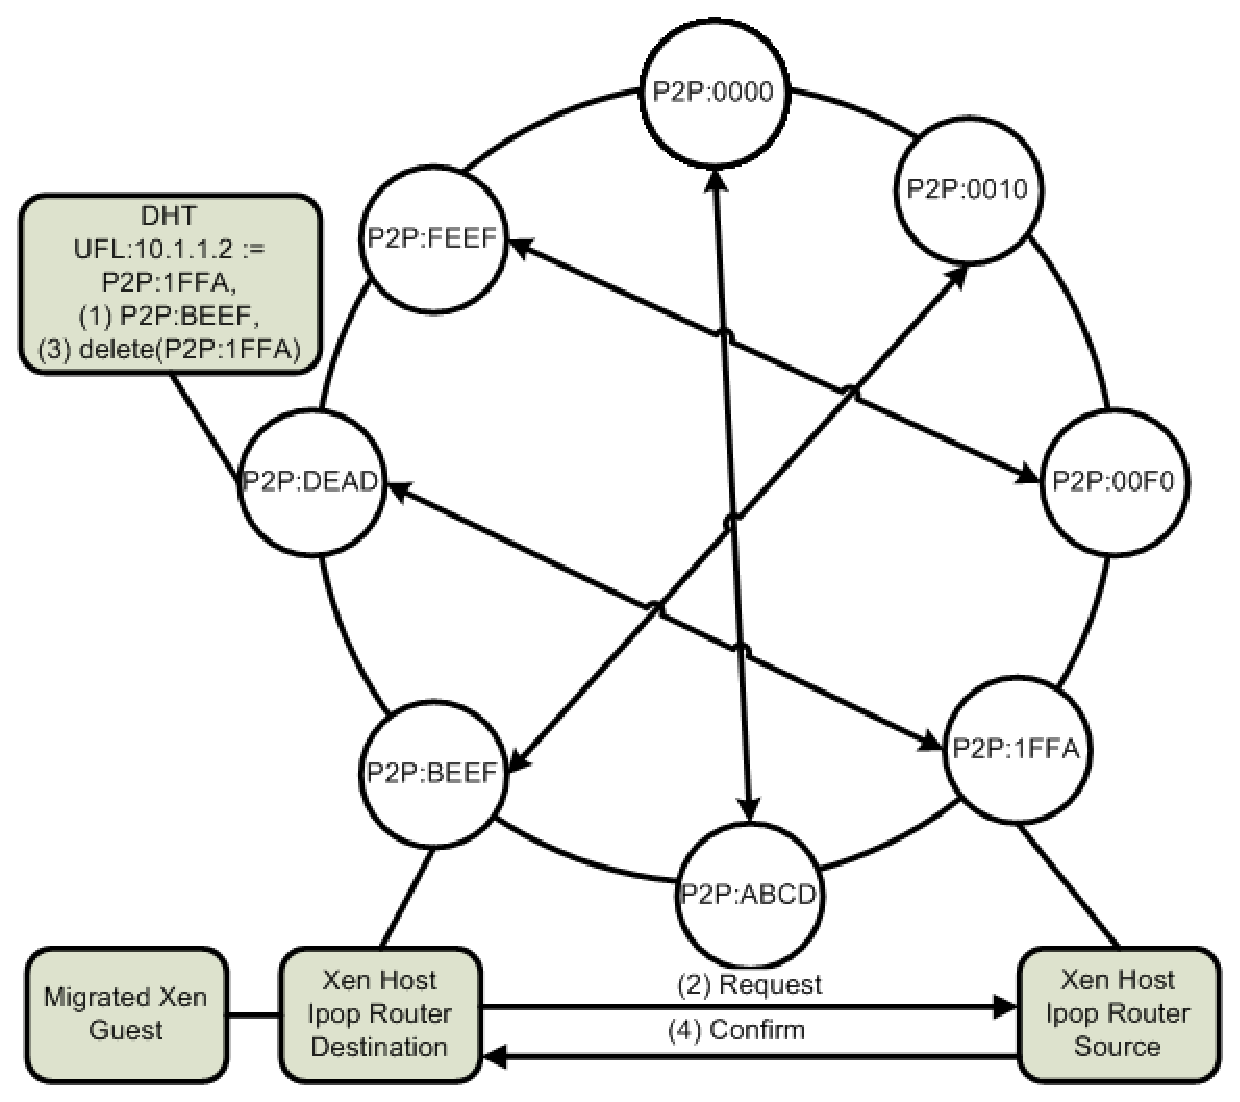
\epsfig{file=figs/Migration.png.eps, width=\textwidth}
\caption[VN Router migration]{The VN operations that occur after a guest (VM)
has been migrated.  (1) The destination retrieves the P2P information of the
source from the DHT and optimistically places its information into the DHT.
(2) The destination requests that the source delete its information from the
DHT.  (3)  The source confirms that the VM is no longer present and performs
the delete.  (4)  The source notifies the destination that its request has
finished successfully.}
\label{fig:migration_ring}
\end{figure}

\begin{figure}
\centering
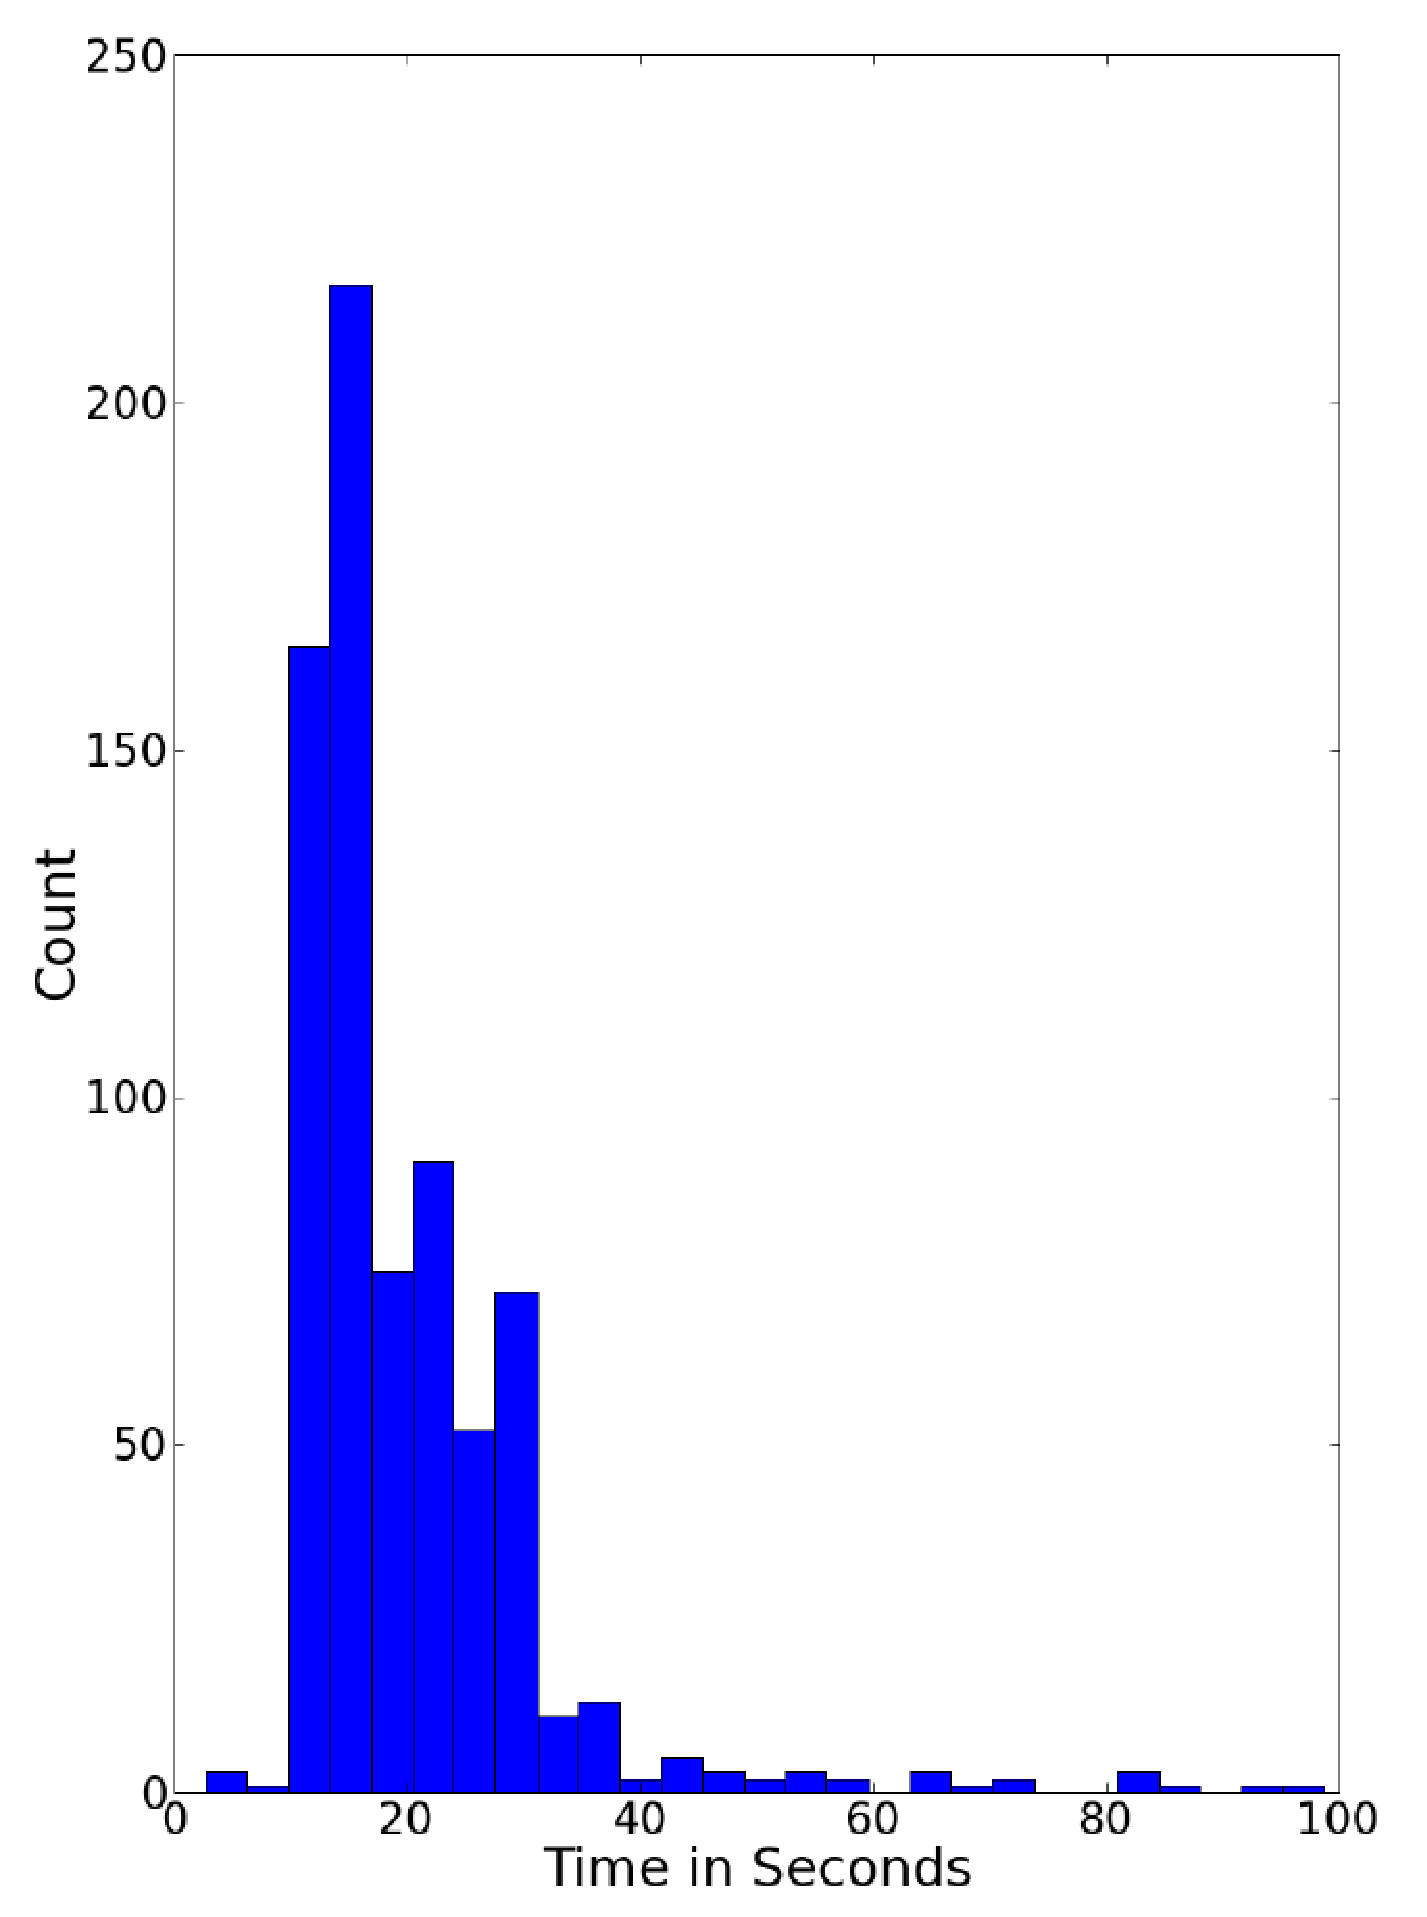
\epsfig{file=figs/migration_results.png.eps, width=3.5in}
\caption[VN Router migration evaluation]{VN Router migration evaluation.  Over
50 different IPs migrated about 10 times each.  The average was 20.11 seconds
with a standard deviation of 10.89.  In this experiment, the majority of this
time comes from VN migration, whereas VM migration requires less than a second.}
\label{fig:mig}
\end{figure}

\section{Evaluation of VPN Network Configuration}

This experiments explores bandwidth and latency in a distributed VPN system to
motivate the usage of P2P links in a VPN.  The VPNs used are include the
prototype (IPOP), OpenVPN, and Hamachi.  OpenVPN represents a typical
centralized VPN, while Hamachi represents a well-tuned P2P-link VPN.  The
evaluation was performed on Amazon EC2 using small instance sized Ubuntu i386
instances to create various sized networks ranging from 1 to 32.  OpenVPN uses
an additional node as the central server and Hamachi has an upper bound of 16
due to limitations in the Linux version at the time of this evaluation.  To
perform bandwidth tests, the instances are booted and query an NFS for the list
virtual IP addresses, peers are ordered such that half the peers are act as
clients and the other half the peers creating a 1 to 1 mapping between all
sets.  Latency and bandwidth tests are performed using netperf's request-reply
and streaming tests respectively.  Prior to the start of the tests, peers have
no knowledge of each other, except the virtual IP addresses, thus connection
startup costs are included in the test.  Test are run for 10 minutes diluting
the connection initiation overhead but represent an example of real usage.
Results from the clients are polled at all locations and averaged together,
though the OpenVPN server is measured separately.  IPOP and OpenVPN use
authenticated 128-bit AES, while Hamachi does not allow configuration of the
security parameters and uses the default Hamachi settings.

\begin{figure}
\centering
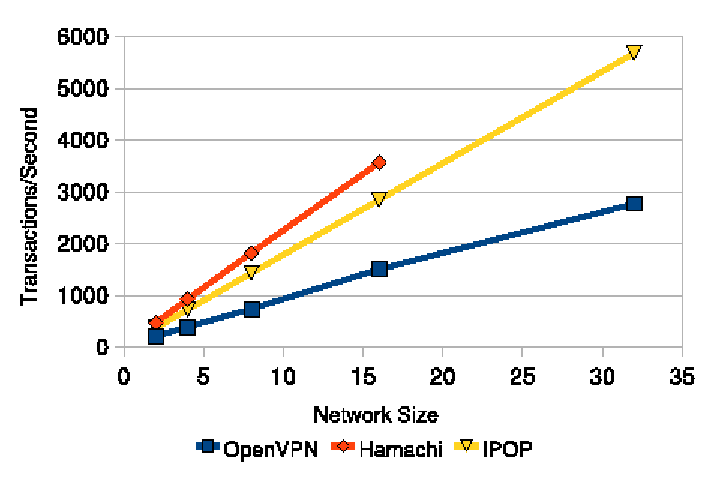
\epsfig{file=figs/latency.eps}
\caption{System transaction rate for various VPN approaches.}
\label{fig:latency}
\end{figure}

Figure \ref{fig:latency} and \ref{fig:bandwidth} present the results for latency
and bandwidth respectively.  Latency is measured in transactions of successful
request/reply messages.  In the latency test, it is obvious that having the
central server increases the delay between the client and server and the results
degrade more quickly as additional peers are added to the system.  In small
systems, OpenVPN shines probably due to optimized software, though as the system
grows, the system bandwidth does not.  By the time 8 peers have entered into
the system, both decentralized approaches perform better than the OpenVPN
solution.  To summarize, decentralized VPN approaches provide better
scalability, which can be immediately noticed by low latency times and, as the
system grows, available bandwidth.

\begin{figure}
\centering
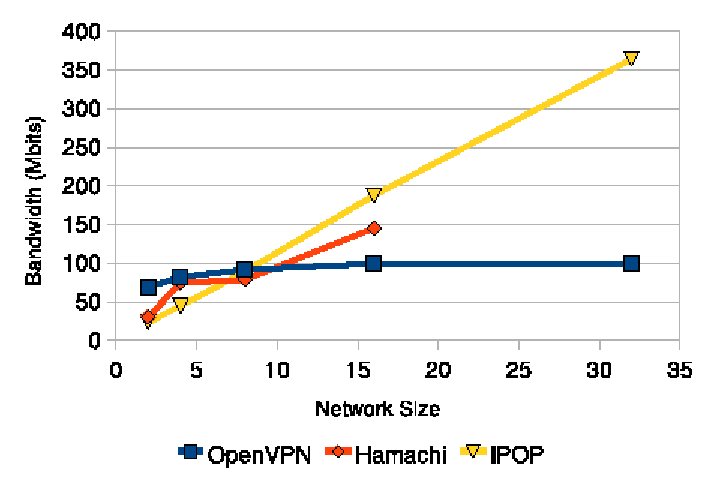
\epsfig{file=figs/bandwidth.eps}
\caption{System bandwidth for various VPN approaches.}
\label{fig:bandwidth}
\end{figure}

\section{Evaluation of VPN Local Configuration}

This section presents an evaluation of the different VN models, using prototype
implementations built upon IPOP.  The grid evaluation simulates a client/server
environment and investigate CPU / networking overheads related with each
approach.  In addition a cloud deployment shows a proof of concept that
connects multiple cloud and local resources as well as evaluation of overhead
of the different approaches in WAN and LAN environments.  In all WAN
experiments, a wide-area IPOP overlay network with approximately 500 overlay
nodes distributed across the world on PlanetLab resources is used to bootstrap
VN connections and to support DHT-based storage and P2P messaging.

The proposed VN models place varying demands on the resources of the systems
involved. The evaluation focuses on CPU as experience suggest that this is the
most significant limiting factor.  As will be presented, the CPU load offered
by these models depends on the bandwidth of the underlying network link, since
a larger bandwidth requires more processing of packets.  The tools for
evaluating these VN models are Netperf and SPECjbb.

Netperf~\cite{netperf} is used to estimate the latency and bandwidth of the
different VN models. The latency is measured by deploying Netperf in the
TCP\_RR mode, which measures the number of 1-byte request-receive transactions
that can be completed in a second. The bandwidth is estimated by running Netperf
in the TCP\_STREAM mode, which is a bulk transfer mode. It should be noted that
in situations where the link bandwidths were asymmetric, Netperf is deployed in
both directions.  Since both latency and bandwidth are dependent on the CPU
comparison, evaluations that include CPU utilization tasks require creating
a baseline first where only Netperf is the only active workload.

SPECjbb~\cite{specjbb} simulates a three-tier web application with all the
clients, the middle tier, and the database running on a single system in a
single address space (inside a JVM). On completion, the benchmark provides the
metric in terms of business of operations per second (bops). The bops score of
the system under test depends on both the CPU and the memory in the system, as
the entire database for the benchmark is held in memory. This benchmark
generates negligible disk activity and no network activity. 

\subsection{On the Grid}

The initial evaluation involves testing a client-server environment.  The
baseline hardware consisted of quad-core 2.3GHz 5140 Xeon with 5 GB memory and
Gigabit network connectivity.  Each VM was allocated 512 MB of RAM and ran
Debian 4.0 using a Linux 2.6.25 kernel.  The client side consisted of 4 VMs on
5 machines.  The server side consisted of 5 VMs on one machine with 4 acting as
servers and 1 acting as a gateway, which was necessary to control bandwidth
into the system, done through the Linux utility \textbf{tc}~\cite{tc}, traffic
control.  In this environment, each server had 5 clients communicating with it.
The setup is shown in Figure~\ref{fig:gridsetup}.

\begin{figure}
\centering
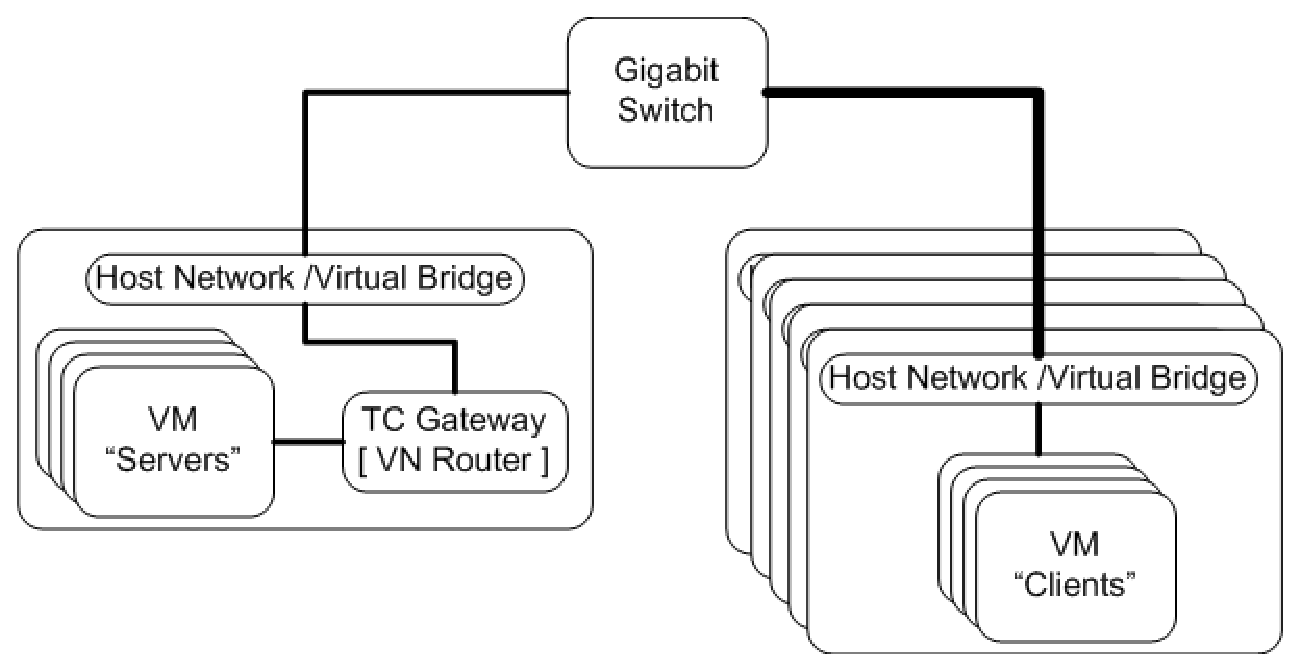
\epsfig{file=figs/grid_setup.png.eps, width=4in}
\caption[Grid evaluation setup]{The system setup for the grid experiments.  The
VM ``Servers'' ran SPECjbb and were also the site for the collection of the
netperf benchmarks.  All the VM ``Servers'' were connected through the TC
Gateway through host-only networking to the VM ``Clients''.  All traffic for
the VM ``Servers'' passes through the TC Gateway, which also doubled as the
Router in the Router experiments.}
\label{fig:gridsetup}
\end{figure}

The maximum bandwidth of 600 Mbps is achieved when neither virtual network nor
traffic shaping are enabled (``no spec.phys'' at 1000 Mbps limit in
Figure~\ref{fig:stream.netperf}), which is only 60\% of the theoretical
maximum.  This limit is most likely the cost of VMMs, specifically the time
required for a packet to traverse both VMMs networking stack as well as the
hosts networking stack.  Another observation was that transactions per second
(Figure~\ref{fig:rr.spec}) do not improve significantly for \textbf{tc}
bandwidth limit above 25 Mbps in all cases; thus focus is on only the relevant
data up to this limit.

\begin{figure}
\centering
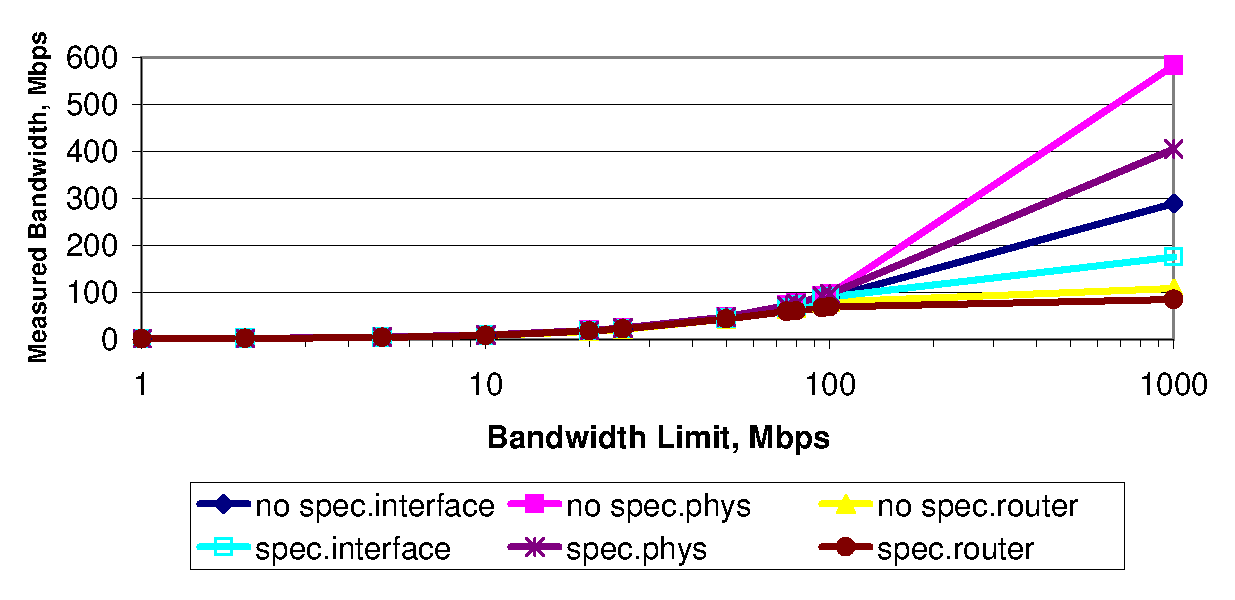
\includegraphics[width=4in]{figs/stream.netperf.jpg.eps}
\caption[Grid Netperf bandwidth evaluation]{Netperf TCP Stream bandwidth
measurements with and without SPECjbb load.  Lines are of the form (no spec,
spec).(phys, interface, router).  Where ``spec'' indicates SPECjbb benchmark is
active, while ``no spec'' indicates that SPECJbb is inactive. ``phys'' implies
the absence of IPOP with benchmarks occurring directly over the ``physical''
network card.  ``interface'' and ``router'' present the results for VN
interface and router models respectively.}
\label{fig:stream.netperf}
\end{figure}

\begin{figure}
\centering
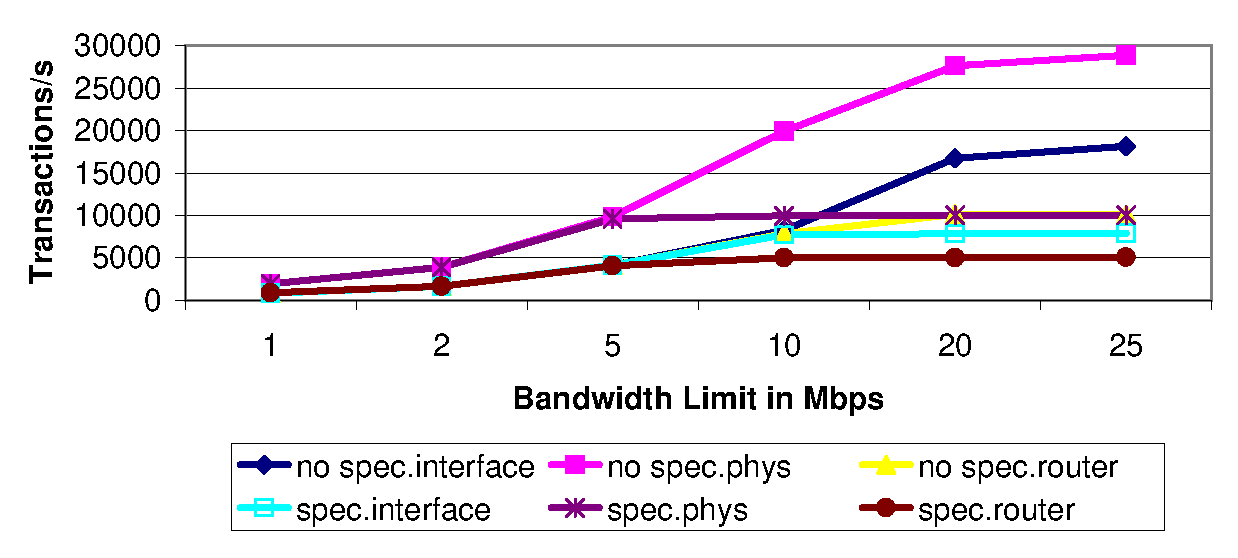
\includegraphics[width=4in]{figs/rr.netperf.jpg.eps}
\caption[Grid Netperf latency evaluation]{Netperf TCP RR latency measurements
with and without SPECjbb load.  Lines are of the form (no spec, spec).(phys,
interface, router).  Where ``spec'' indicates SPECjbb benchmark is active,
while ``no spec'' indicates that SPECJbb is inactive. ``phys'' implies the
absence of IPOP with benchmarks occurring directly over the ``physical''
network card.  ``interface'' and ``router'' present the results for VN
interface and router models respectively.}
\label{fig:rr.netperf}
\end{figure}


Distinguishing features of the different VN models include the following.
Figure~\ref{fig:stream.netperf} shows that bandwidth in all VN models is
comparable with traffic control limit up to 75 Mbps. Beyond this point, the
interface model achieves better bandwidth than the router model (VN processing
is distributed across multiple processes); the spec/no spec ratio in the router
model is smaller than in the interface model because there is less resource
contention caused by VN processing on end nodes. For the same reason, the
router tends to achieve better SPEC results (Figure~\ref{fig:stream.spec}) than
the interface.  Figure~\ref{fig:rr.netperf} shows that the router performs
poorly compared to the interface model in terms of transactions/second, though
it achieves a better ratio of SPECjbb score (Figure~\ref{fig:rr.spec}) to
transactions than the interface at constrained bandwidths (less than 5 Mbps).

\begin{figure}
\centering
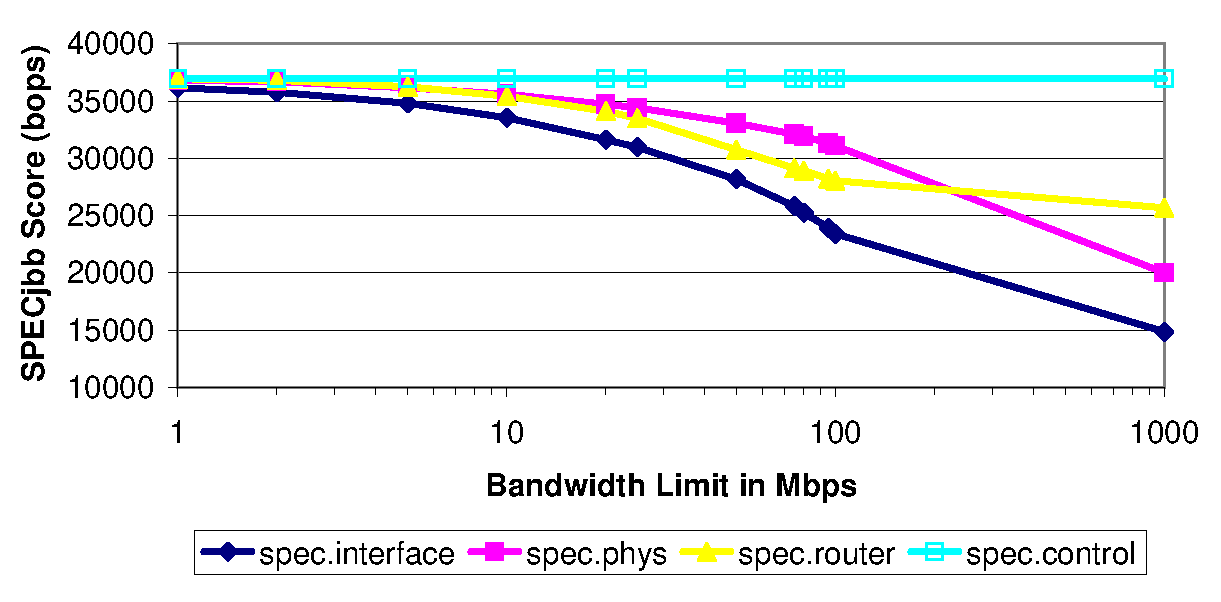
\includegraphics[width=4in]{figs/stream.spec.jpg.eps}
\caption[Grid SPECjbb evaluation, Stream load]{SPECjbb scores with and without
Netperf Stream load.  Lines are of the form spec.(control, phys, interface,
router).  ``spec'' implies that SPECJbb executes in all tests.  In ``control''
Netperf is inactive, that is, it is the maximum attainable value for SPECJbb.
``phys'' implies the absence of IPOP with benchmarks occurring directly over
the ``physical'' network card.  ``interface'' and ``router'' present the
results for VN interface and router models respectively.}
\label{fig:stream.spec}
\end{figure}


\begin{figure}
\centering
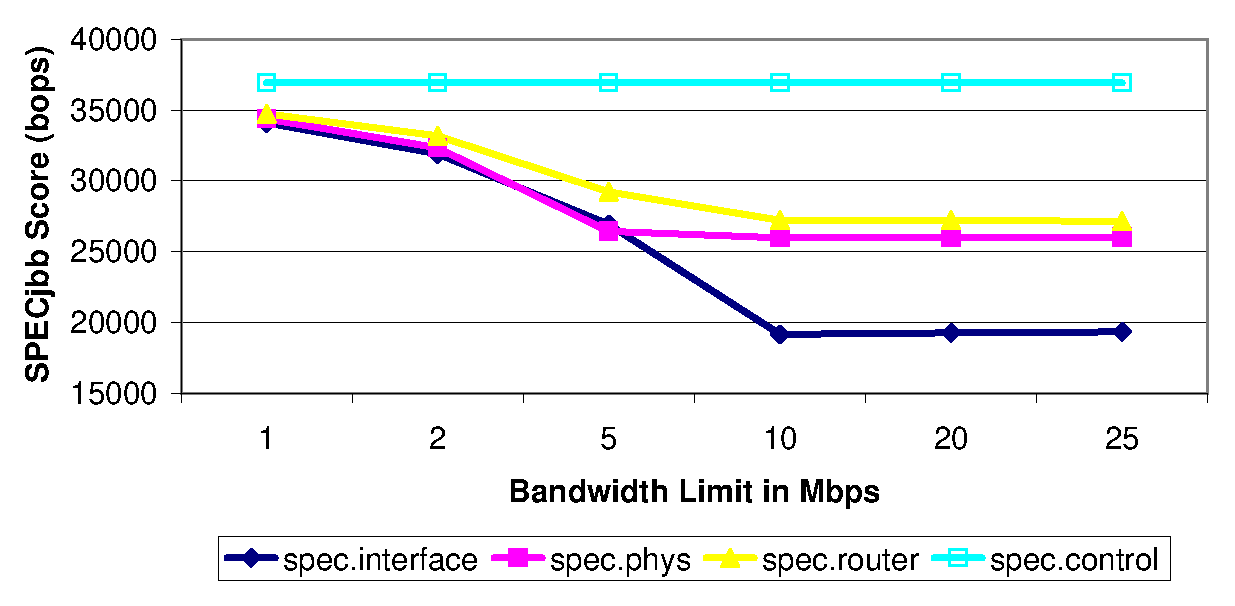
\includegraphics[width=4in]{figs/rr.spec.jpg.eps}
\caption[Grid SPECjbb evaluation, RR load]{SPECjbb scores with and without
Netperf RR load.  Lines are of the form spec.(control, phys, interface,
router).  ``spec'' implies that SPECJbb executes in all tests.  In ``control''
Netperf is inactive, that is, it is the maximum attainable value for SPECJbb.
``phys'' implies the absence of IPOP with benchmarks occurring directly over
the ``physical'' network card.  ``interface'' and ``router'' present the
results for VN interface and router models respectively.}
\label{fig:rr.spec}
\end{figure}

The hybrid method was tested, and results were nearly identical to those of the
interface, from the point of view of the WAN part of the VN, it is the same
architecture.  These results are not reported in the plots as they add little
value and further obfuscate the results.

The bandwidth cap observed in the router approach reflects the performance
achieved by the current prototype of the router, subject to VM overheads. The
use of VM is an assumption that is valid in the domain of cloud computing where
all resources run in a VM. This experiment focused on the interplay between
resource consumption by overlay routers and application performance.  Optimized
user-level overlay routers running on dedicated physical machines have been
reported to achieve performance near Gbit/s in related work~\cite{vine2}.

One thing that left unevaluated that may provide more interesting data would be
providing the VN router dedicated hardware.  In the test environments, this was
infeasible, because all but one of the machines in the lab run VMware Server 1,
which has a bug with setting the virtual network card in promiscuous mode.
This effectively makes it impossible for a VM to be a VN router as no packets
will ever make their way into the VM, as the VMM will reject all packets.  As
such, the machines hosting the servers had VMware Server 2, which does allow
setting a network interface into promiscuous mode.

\subsection{In the Clouds}

The goal of this experiment is to demonstrate the feasibility of connecting
multiple cloud providers as well as local resources together through virtual
networking.  The sites chosen for evaluation were local resources at University
of Florida and cloud resources provided by Amazon EC2 and GoGrid.  A
qualitative observation here was that the differences in the networking
infrastructure exposed by different cloud providers reinforce the importance of
the virtual network to allow flexibility in how end nodes are connected.
Specific network configurations for the clouds were as follows:

\begin{itemize}

\item Amazon EC2 provides static IP networking (public and private), no
Ethernet connectivity, and no ability to reconfigure IP addresses for network.
Currently, only the VN interface model is supported.

\item GoGrid provides 3 interfaces (one public, statically configured, and two
private, which can be configured in any manner); the 2 private interfaces are
on separate VLANs supporting Ethernet connectivity. The VN interface, router,
and hybrid models are supported.

\end{itemize}

This experiment narrows down the performance evaluation to focus on WAN and LAN
performance of VNs in cloud environments and consider Netperf single
client-server interactions only. Amazon only supports Interface mode, thus it
is only evaluated in the WAN experiment. It has been observed that, within
Amazon, the VN is able to self-organize direct overlay connections~\cite{wow}.
Each test was run 5 times for 30 seconds, the standard deviation for all
results was less than 1.  Because of this, only the average is presented in
Table~\ref{tab:cloud-wan}.

\begin{center}
\begin{table}
\caption[WAN Results for inter-cloud networking]{WAN Results for inter-cloud
networking.  Stream is in Mbs and RR is in trans/s (The inverse of trans/s
would be equal to the average latency).}
\begin{tabular*}{\textwidth}{@{\extracolsep{\fill}}
l
S[table-format=2.2,table-number-alignment=right]
S[table-format=2.2,table-number-alignment=right]
S[table-format=2.2,table-number-alignment=right]
@{}
}

\hline & 
\multicolumn{1}{c}{EC2 / UF} &
\multicolumn{1}{c}{EC2 / GoGrid} &
\multicolumn{1}{c}{UF / GoGrid} \\ \hline \hline

Stream Phys & 89.21 & 35.93 & 30.17\\ \hline
Stream VN & 75.31 & 19.21 & 25.65\\ \hline
RR Phys & 13.35 & 11.09  & 9.97 \\ \hline
RR VN & 13.33 & 10.69 & 9.76 \\ \hline

\end{tabular*}
\label{tab:cloud-wan}
\end{table}
\end{center}

It can be seen in Table~\ref{tab:cloud-wan} that the VN adds little overhead in
the Netperf-RR experiment. Between UF and GoGrid as well as between UF and
Amazon EC2, the overhead for the Stream experiment was about 15\%.  This may be
attributed to the additional per-packet overhead of the VN and the small MTU
set for the VN interface (1200).  The MTU, or maximum transmission unit, is the
largest packet that is sent from an interface.  IPOP conservatively limits the
VN MTU to 1200 down from the default 1500 to allow for overlay headers and to
work properly with poorly configured routers, which has encountered in
practical deployments.  A more dynamic MTU, which will improve performance, is
left as future work.  The EC2 / GoGrid experiment had greater overhead which
could possibly be attributed to by the VM encapsulation of cloud resources.

Table~\ref{tab:cloud-lan} shows that some of the performance expectations for
the different models in a LAN were accurately predicted while others were not
so clear.  Stream results match the expectation that VN models hybrid and
router bypass virtualization and get near physical speeds, whereas interface
does not.  Interestingly, RR had rather poor results for Router and Hybrid
though further testing seems to indicate that this is an issue of using the
VLAN connected network interfaces as opposed to the public network connected
interface.

\begin{center}
\begin{table}
\caption[LAN results performed at GoGrid]{LAN results performed at GoGrid.
Stream is in Mbs and RR is in trans/s.  Interface and Physical used the eth0
NIC, while Router and Hybrid used eth1.  Different VLANs may give different
results.}
\begin{tabular*}{\textwidth}{@{\extracolsep{\fill}}
l
S[table-format=4.0,table-number-alignment=right]
S[table-format=4.0,table-number-alignment=right]
S[table-format=4.0,table-number-alignment=right]
S[table-format=4.0,table-number-alignment=right]
@{}
}

\hline & 
\multicolumn{1}{c}{VN Interface} &
\multicolumn{1}{c}{VN Router} &
\multicolumn{1}{c}{VN Hybrid} &
\multicolumn{1}{c}{Physical} \\ \hline \hline
Stream & 109 & 325 & 324 & 327 \\ \hline
RR & 1863 & 2277 & 2253 & 3121 \\ \hline
\end{tabular*}
\label{tab:cloud-lan}
\end{table}
\end{center}

\begin{center}
\singlespacing{
\footnotesize{
\begin{longtable}{p{.8in}p{1.15in}p{1.3in}p{1.25in}p{1.25in}}
\caption[Virtual Network Comparison]{Virtual Network Comparison} \\

\hline & Overlay & Routing & Configuration & Miscellaneous \\ \hline \hline
\endfirsthead

\multicolumn{5}{l}{\normalsize{Table \ref{tab:virtual_networks}. Continued}}\\
\hline & Overlay & Routing & Configuration & Miscellaneous \\ \hline \hline
\endhead

\hline
IPOP
&
%Overlay
Structured P2P overlay with O(Log N) routing hops, where N is the size of P2P
network. Self-optimizing shortcuts and STUN-based NAT traversal.
&
%Routing
Mapping stored in DHT resolves virtual IP address to P2P address. Virtual
network packets are routed to corresponding P2P address.
&
%Configuration
Each machine runs P2P VPN software with a dynamic IP address in a common subnet.
Common configuration shared amongst all hosts.
&
% Misc.
Supports encrypted P2P links and end-to-end VPN tunnels (unpublished work).
Migration possible; routes self-configure without user intervention, product of
the P2P overlay.
\\ \hline
N2N
&
%Overlay
Unstructured P2P network, super nodes provide control paths, forms direct
connections for data.
&
%Routing
Broadcast for discovery and overlay for control.  No organization, no guarantees
about routing time.
&
%Configuration
Requires N2N software at each host, must connect to a super node.  Supports
layer 2 Ethernet network.
&
% Misc.
Supports shared secrets to create private tunnels between edges.  Migration not
discussed, but potentially free due to layer 2 approach.
\\ \hline
OCALA
&
%Overlay
Not tied to any specific overlay, layer 3 middleware.
&
%Routing
Based upon chosen overlay.
&
%Configuration
Requires OCALA stack, overlay configuration, and IP to overlay mapping.
&
% Misc.
Security is overlay based or SSH tunnels.  Migration not mentioned.
\\ \hline
SoftUDC VNET
&
%Overlay
Decentralized with explicitly configured overlay routes.
&
%Routing
Broadcast for discovery.
&
%Configuration
Requires software on each host and one proxy per site.  Layer 2 networking.
&
%Misc.
Security is not discussed nor is wide-area migration.
\\ \hline
ViNe
&
%Overlay
ViNe authority configures global network descriptor table (GNDT) explicitly at
each router. Supports proxying to one location through another and NAT traversal.
&
%Routing
GNDT provides overlay routes for all routers in overlay.
&
%Configuration
Each subnet is allocated a single router.  Each host must be configured for
regular and ViNe networks, but no VN software needed on host.
&
% Misc.
Supports encrypted tunnels between ViNe routers, migration not discussed.
\\ \hline
Violin
&
%Overlay
Decentralized network with statically configured overlay routes.
&
%Routing
Broadcast discovery for Ethernet, static routes for IP subnet.
&
%Configuration
Virtual hosts connect VMs to the VN.  Hosts connect to virtual switches or
proxies (gateways).  Switches connect to proxies.  Sites are typically
allocated an IP address space.
&
% Misc.
Security potentially through the use of SSH Tunnels.  Migration possible;
requires reconfiguration of switches. 
\\ \hline
Virtuoso VNET
&
%Overlay
Decentralized with explicitly configured overlay routes.
&
%Routing
Broadcast for discovery.  Bridging learns paths after initial discovery.  Virtual
network packets are routed between VNET proxies.  Can be configured manually.
&
%Configuration
Each site runs a proxy providing Ethernet bridge to other proxies.  VM hosts
forward packets to local proxy.  Proxies configured to connect to other proxies.
&
% Misc.
Security through the use of SSL and SSH Tunnels.  Layer 3 migration, product of
layer 2 virtualization.
\\ \hline
OpenVPN
&
%Overlay
Centralized
&
%Routing
Central server
&
%Configuration
Servers manually configured to connect with each other.  Clients randomly select
server from pre-shared list
&
%Misc
All communication traverses central server, end to end traffic by default is not
protected from central server
\\ \hline
Tinc and CloudVPN
&
%Overlay
Decentralized with explicitly configured overlay routes
&
%Routing
Broadcast for discovery, messages traverse overlay
&
%Configuration
Manual configuration
&
%Misc
NAT traversal through relays only
\\ \hline
Hamachi
&
%Overlay
Centralized Discovery, P2P links
&
%Routing
Peers establish security links and end point information from a central
server, attempt to form direct connections, if fails, relay through central
server
&
%Configuration
Select a network to join or create and specify a password, communicates with a
centralized server to manage the VPN
&
%Misc
Lacks portability, Linux version out of date, inability to run external relay
servers, UDP NAT traversal
\\ \hline
GBridge
&
%Overlay
Centralized Discovery, P2P links
&
%Routing
Peers establish security links and end point information from a central
server, attempt to form direct connections, if fails, relay through central
server
&
%Configuration
Select a network to join or create and specify a password, communicates with a
centralized server to manage the VPN
&
%Misc
Lacks portability and inability to run external relay servers, uses TCP NAT
traversal
\\ \hline
Wippien
&
%Overlay
Centralized Discovery, P2P links
&
%Routing
Peers discover and authenticate each other through XMPP chat server, security
provided unknown, peers attempt to form direct connections with each other, if
that fails, no communication
&
%Configuration
All peers must be members of associated XMPP chat rooms and be connected to the
chat
&
Requires a GUI, difficulty penetrating NATs, claims to be open source though
most of the code is unavailable, Linux client out of date and does not support
NAT traversal
%Misc
\\ \hline
P2PVPN
&
%Overlay
Centralized Discovery, P2P links
&
%Routing
Peers discover each other through a BitTorrent tracker and attempt to form
direct links with each other, attempts to form all-to-all connectivity, if
direct links are unavailable, indirect links can be used to forward packets
&
%Configuration
Peers must join the same tracker and use common shared secret
&
%Misc
Work in progress to make more unstructured, currently a cross between
centralized and decentralized
\\ \hline
\label{tab:virtual_networks}
\end{longtable} } }
\end{center}

\chapter{BOOTSTRAPPING PRIVATE OVERLAYS}
\label{chap:bootstrapping}

While P2P overlays provide a scalable, resilient, and self-configuring platform
for distributed applications, their adoption rate for use across the Internet
has been slow outside of large-scale systems, such as data distribution and
communication.  General use of decentralized, P2P (peer-to-peer) applications
targeting homes and small/medium businesses (SMBs) has been limited in large
part due to difficulty in decentralized discovery of P2P systems, the bootstrap
problem, further inhibited by constrained network conditions due to firewalls
and NATs (network address translators).  While these environments could benefit
from P2P, many of these users lack the resources or expertise necessary to
bootstrap private\footnote{In the context of this chapter, private implies that
the overlay's purpose is not for general use. Once established, such overlays
can support privacy in communication; however, overlay security is beyond the
scope of this chapter and covered in more depth in chapter\ref{chap:security}.}
P2P overlays particularly when the membership is unsteady and distributed
across wide-area network environments where a significant amount of (or all)
peers may be unable to initiate direct communication with each other due to
firewalls and NAT (network address translation).

Examples of large-scale P2P systems include Skype, BitTorrent, and Gnutella.
Skype is a voice over P2P system, whereas BitTorrent and Gnutella are used for
file sharing.  The bootstrapping in these systems typically relies on overlay
maintainers using high availability systems for bootstrapping, bundling their
connection information with the application distribution.  The application then
uses theses servers during the initialization phase to connect with other peers
in the system.  Alternatively, some services constantly crawl the network and
place peer lists on dedicated web sites. A new peer wishing to join the network
queries the web site and then attempts to connect to the peers on this list.

In smaller-scale systems, P2P interests focus on decentralization.  For
example, users may desire to run an application at many distributed sites, but
the application lacks dedicated central servers to provide discovery or
rendezvous service for peers.  In contrast, dedicated, centralized P2P service
providers, such as LogMeIn's Hamachi, a P2P VPN (virtual private network), may
collect usage data, which the users may wish to remain private, or are not free
for use.

Many applications make sense for small-scale overlay usage, including
multiplayer games, especially those that lack dedicated online services;
private data sharing; and distributed file systems.  Clearly, a small P2P
system could be bootstrapped by one or more users of the system running on
public addresses, distributing addresses out-of-band, instructing their peers
to add that address to their P2P application, and then initiate bootstrapping;
but these types of situations are an exception and not the norm.  Ultimately,
the users would be enhanced significantly through approaches that can make
decentralized bootstrapping transparent through minimal and intuitive
interaction with the P2P component.

\begin{figure}
\centering
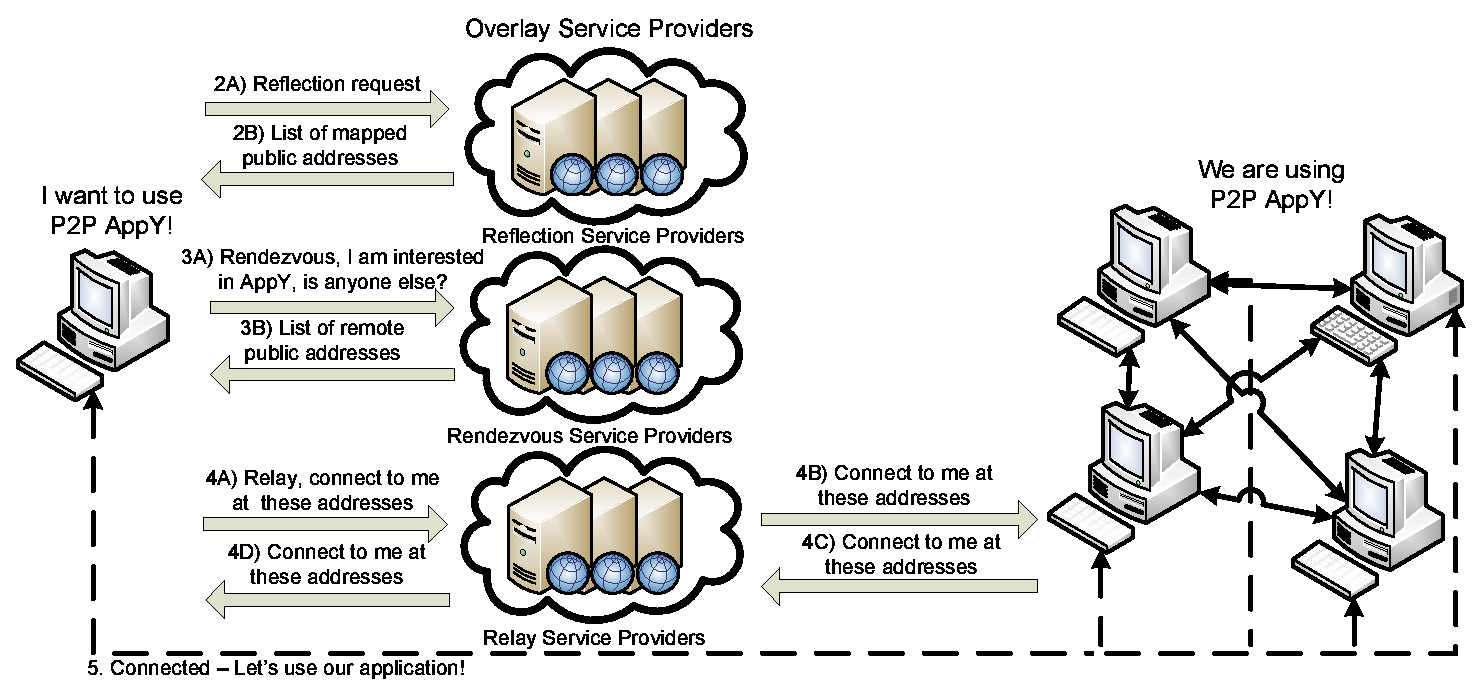
\epsfig{file=figs/bootstrap.eps, width=5.5in}
\caption{Bootstrapping a P2P system using an existing (generic) overlay.}
\label{fig:bootstrap}
\end{figure}

The basic bootstrapping process can be broken down into two components: finding
and connecting to an active peer in the system.  When a node starts, it
contacts various bootstrap servers, until it successfully connects with one,
upon which they exchange information.  The bootstrap server may inquire into
the overlay for the best set of peers for the new peer and respond with that
information or it may respond with its existing neighbor set.  At which point,
the peer attempts to connect with those peers.  This process continues
aggressively until the peer arrives at a steady state, either connecting with a
specific set of or a number of peers.  Afterwards, the P2P logic becomes
passive, only reacting to churn from new incoming or outgoing peers.

Overlay support for constrained peers, i.e., those behind NATs and restrictive
firewalls, requires additional features to support all-to-all connectivity for
peers in the overlay.  The instantiation of P2P systems for private use could
become overly burdensome, potentially relying on significant human interaction
to bootstrap them, for example, by relaying connection information through
phone calls and e-mail.  Even if this is feasible, this sort of interaction is
undesirable.  P2P systems should be self-discovering, minimizing the amount of
work users need to do in order to take advantage of them, a feature stressed by
ad-hoc systems.  In addition, these approaches may rely on centralized
components; if they become unavailable, which is a possibility since most users
lack the expertise in configuring highly available systems, the system will not
be accessible.

To address this, I have explored the possibility of using existing public
overlays as a means to bootstrap private overlays.  There are many existing
public overlays with high availability, such as Skype, Gnutella, XMPP
(Extensible Messaging and Presence Protocol), and BitTorrent; by leveraging
these systems, system integrators can easily enable users to seamlessly
bootstrap their own private P2P systems.  In the preceding paragraphs, I have
identified the components necessary for bootstrapping a homogeneous system; in
the following, I will expand them for environments to support the bootstrapping
of a private overlay from a public overlay with consideration for network
constrained peers.  The public overlay must support the following mechanisms as
illustrated in Figure~\ref{fig:bootstrap}:

\begin{enumerate}

\item REFLECTION. A method for obtaining global application and IP addresses or
identifier for a peer that can be shared with others to enable direct
communication.

\item RELAYING. A method for peers to exchange arbitrary data, when a direct IP
link is unavailable.

\item RENDEZVOUS. A method for identifying peers interested in the same P2P
service.

\end{enumerate}

This work motivates from the belief that while small-scale P2P systems are
attractive for decentralized systems, the overheads relating to creating and
maintaining bootstrap services make them unfeasible.  A public overlay can be
used to transparently bootstrap a private overlay with minimal user
interaction.

The requirements are presented and verified in the context of two prototype
implementations: a XMPP / Jabber~\cite{xmpp} and Brunet~\cite{brunet}.
XMPP-based overlays are commonly used as chat portals, such as GoogleTalk and
Facebook Chat.  XMPP also supports an overlay amongst servers forming through
the XMPP Federation, which allows inter-domain communication amongst chat
peers, so that users from various XMPP servers can communicate with each other.
Brunet provides generic P2P abstractions as well as an implementation of the
Symphony structured overlay.  I present the architecture for these systems, the
lessons learned in constructing and evaluating them, and provide an analysis of
the latency to establish peer connectivity in a small-scale private Brunet
overlay with NAT-constrained nodes.

The organization of this chapter follows.  Section~\ref{bs:background}
overviews existing solutions to the bootstrapping problem, and NAT challenges
in P2P systems.  Section~\ref{bs:overview} presents a survey of overlays,
applying the requirements for private overlay bootstrapping to them, and then
show in detail how they can be applied to Brunet and XMPP.  My implementation
is described in Section~\ref{bs:implementation}.  In
Section~\ref{bs:evaluations}, I perform a timing evaluation of bootstrapping
overlays using my prototype on PlanetLab and discuss experiences in deploying
the system.  

\section{Current Bootstrap Solutions}
\label{bs:background}

As described in the introduction, the simple case of bootstrapping is limited
to one peer attempting to find an active peer in the overlay in order for
itself to become a member.  The large-scale providers have resources not
readily available to small-scale overlays.  This section reviews existing
techniques and those being developed and describes their application to
small-scale systems.

When using dedicated bootstrap overlays, a service provider hosts one or more
bootstrap resources.  Peers desiring to join the overlay query bootstrap nodes,
until a successful connection is made to one.  The bootstrap server will then
assist in connecting the peer to other nodes in the P2P system.  Bootstrap
nodes are either packaged with the application at distribution time or through
a meta data file, such as in BitTorrent.  Drawbacks to this approach for small,
ad-hoc pools include that the same server would have to be used every time to
bootstrap the system, or users would have to reconfigure their software to
connect to new bootstrap servers over time; at least one peer must have a
publicly accessible address; and a bootstrap server can become a single point
of failure.

Another commonly used approach for large-scale systems is the use of a host
cache~\cite{host_cache}.  Clients post current connection information to
dedicated web services, a host cache, that in turn communicate with other host
caches.  For small, ad-hoc networks, a host cache acts no differently than a
centralized rendezvous point, requiring that at least one peer has a publicly
accessible address.

``P2P VPN's''~\cite{p2pvpn} use of a BitTorrent tracker is similar to the host
cache concept.  The tracker hosts file meta data and peers involved in sharing.
For the VPN, the peer registers a virtual file used to organize the peers, a
form of rendezvous.  Each peer in the VPN queries the tracker regarding the
file, registers its IP address, and receives other active ``sharers'' IP
addresses.  Peers on public addresses or using UPnP (universal plug and play)
are able to receive incoming connections from all other peers.  The problem
with this approach is that it is heavily user-driven.  A user must register
with each BitTorrent tracker individually and maintain a connection with each
of them, in order to handle cases where BitTorrent trackers go offline.  In
addition, this does not use the BitTorrent trackers in a normal fashion, so it
may be banned by tracker hosts.

Research has shown that peers can use the locality properties of recent IP
(Internet Protocol) addresses in a large-scale P2P system to make intelligent
guesses about other peers in the P2P system using an approach called random
probing~\cite{bootstrapping_p2p, locality_aware}.  The results show that, in a
network of tens to hundreds of thousands of peers, a bootstrapping peer can
find an active peer in 100 guesses to 2,000 guesses, depending on the overlay.
The approach does not really apply well to small-scale systems, especially when
peers are constrained by NATs and firewalls.

Rather than distribute an IP address, which points explicitly to some location
in the Internet, a small P2P network can apply a name abstraction around one
peer in the overlay using Dynamic DNS~\cite{bootstrapping_ddns} (domain name
service).  Peers share a DNS entry, which points to a bootstrap server.  When
the peers detect that the bootstrap server is offline, at random time intervals
they will update the DNS entry with their own.  The application of this
approach is well-suited to small, ad-hoc groups, as the service could be
distributed across multiple Dynamic DNS registrations.  However, sharing a DNS
entry requires trusting all peers in the overlay, making it easy for malicious
peers to inhibit system bootstrapping.  Also the approach requires that at
least one peer be publicly addressable; if a non-publicly addressable peer
updates the cache inadvertently, it could delay or permanently prevent peers
from creating a P2P system.  The results reported in~\cite{bootstrapping_ddns}
were simulation-based and did not determine how well a dynamic DNS handles
rapid changing of name to IP mappings.

IP supports multicasting to groups interested in a common service.  In the case
of bootstrapping a P2P system~\cite{pastry, locality_aware}, all peers would be
members of a specific group.  When a new peer comes online, it queries the
group for connection information and connects to those that respond.  The
approach, by itself, requires that all peers are located in a multicast capable
network, restricting this approach typically to local area networks.

A large-scale structured overlay~\cite{one_ring, p2p_bootstrap} could enable
peers to publish their information into a dedicated location for their service
or application and then query that list to obtain a list of online peers.
Peers could search for other peers in their overlay and connect with them using
their connection information.  Since the service would be a large-scale system,
it could easily be bootstrapped by a dedicated bootstrap or host caches.  As it
stands, the described works were position papers and the systems have not been
fully fleshed out.  The primary challenge in relationship to small, ad-hoc
networks is that it lacks details bootstrapping of peers behind NATs into
overlays as it provides only a means for rendezvous and not reflection nor
relaying.

\section{Core Requirements}
\label{bs:overview}

As presented in the preceding sections, a solution to bootstrapping small P2P
overlays must address several challenges, namely reflection, rendezvous, and
relaying.  This section presents a generic solution to this problem.  The basis
for my solution is reusing existing, free-to-join public overlay.  In order to
support these features the public overlay must have mechanisms for peers to
obtain a public network identity (reflection); search for other peers that are
bootstrapping the same P2P service (rendezvous); and send messages to peers
through the overlay (relaying).  These are the minimum requirements to
bootstrap a decentralized, P2P system when all peers are behind NATs.

\subsection{Reflection}
\label{bs:reflection}

Reflection provides a peer with a globally-addressable identifier for receiving
incoming messages from other peers.  Without reflection, peers on different
networks with non-public addresses are unable to communicate directly with each
other.  Reflection is not limited to IP.  For example, when a peer joins a
service, such as a chat application or a P2P system, the overlay provides a
unique identifier, which also serves as a form of reflection.

In IP communication, reflection enables NAT traversal.  The simplest method for
NAT traversal relies on obtaining the public information for an existing UDP
(user datagram protocol) socket and then sharing that with other peers.  This
behavior can be supported through either local service or remote assistance.
The local approach approach relies on having a router with a public IP address
supporting either UPnP~\cite{upnp} or port forwarding / tracking.  In many
cases, UPnP is not enabled by default and in most commercial venues it will
rarely be enabled.  Port forwarding / tracking requires non-trivial router
configuration, outside the comfort range of many individuals and is not uniform
across routers.  A peer using UPnP needs no further services, as UPnP enables a
peer to set and obtain both public IP address and port mappings.  Port
forwarding and tracking mechanisms still require that the user obtains and
inputs into the application their public IP address or use in-band assistance
described next.

In the remotely assisted scenario, a peer first sends a message to a reflection
provider, perhaps using STUN~\cite{stun_rfc} (Simple Traversal of UDP through
NATs).  The response from the provider tells the peer from which IP address and
port the message was sent.  In the case of all cone NATs, this will create a
binding so that the peer can then share that IP address and port with other
peers behind NATs.  When the two peers communicate simultaneously, all types of
cone NATs can be traversed; the timing of messages needs to be carefully
considered, however, since NAT mappings may change over time.  So long as one
peer is behind a cone NAT, NAT traversal using this mechanism is possible.  The
situation becomes complicated when both peers are behind symmetric NATs, or
when either one of them have a firewall preventing UDP communication.

Peers behind symmetric NATs cannot easily communicate with each other, since
there is no relation between remote hosts and ports and local ports.  Further
complicating the matter is that there are various types of symmetric NATs,
having behaviors similar to the various cone NAT types. In~\cite{ice} the
authors describe methods to traverse these NATs so long as there is a
predictable pattern to port selection.  

Unlike UDP, TCP (transmission control packet) NAT traversal is complicated by
the state associated with TCP.  In many systems, the socket API (application
programming interface) can be used to enable a peer to both listen for incoming
connections and form outgoing connections using the same local addressing
information.  According to~\cite{ice-tcp}, this method works for various types
of systems though the success rate on NATs is low, 40\%.  Other mechanisms rely
on out-of-band communication~\cite{pvc}, or use of complicated predictive
models~\cite{tcp-hole-punching}.

\subsection{Relaying}
\label{bs:relay}

NAT traversal services only deal with one aspect of the bootstrap problem:
reflection.  That is, peers are able to obtain a public address for receiving
incoming connections with no means for to exchange addresses with other peers
nor perform a simultaneous open to traverse restrictive NATs.  To address this
issue, many systems incorporate these NAT traversal libraries while using
intermediaries to exchange addresses as a method of relaying.  Another form of
relaying exists when two peers are unable to form direct IP connections with
each other and route data messages between a third-party.

The most common method for relaying in IP is the use of TURN~\cite{turn}
(Traversal Using Relay NAT).  A peer using TURN obtains a public IP address and
port that can be used as a forwarding address.  When a remote peer sends to
this address, the TURN server will forward the response to the peer who has
been allocated that mapping.  The lack of abstraction in TURN makes the system
heavily centralized, making its application in small-scale systems complicated.  

In overlays, peers typically have an abstracted identifier that does not
associate them with a single server enabling more decentralized approaches to
relaying.  When a remote peer sends a message to the identifier, the overlay
should translate the identifier into network level addresses and forward it to
the destination.  Because of this restriction, messages sent by relaying cannot
have expectations more than that of sending a packet by UDP.  In other words, a
packet will either be received in a reasonable amount of time or not at all.
Support for reliability, streaming, and flow control, if necessary, must be
provided in user-space.

Finally, the service should be asynchronous or event driven.  The previous
requirements would allow peers to relay through a message board or even by
posting messages to a DHT.  The problem with these two approaches is that peers
may very well communicate for long periods of time using these services.  That
means the potential for posting large amounts of data to a service that will
retain it and constantly querying the service to determine if an update is
available.  Both of these are highly undesirable and may be viewed as denial of
service or spam attacks.

\subsection{Rendezvous}
\label{bs:rendezvous}

A rendezvous service allows peers to discover the global identifier of peers
interested in the same service.  For any given overlay, a naive approach for
rendezvous is the use of a broadcast query or random probing to determine if
any other peers are using the same service.  This approach is unreasonable,
depending on the size of the bootstrap overlay compared to the destination
overlay, it may be very difficult to find another peer, some or all peers may
be behind NATs and unreachable without assistance, and in the worst case
scenario a malicious attacker could be waiting for bootstrap requests into the
system.

Rather than attempt to make a single unified rendezvous technique, each overlay
style usually provide an efficient means for rendezvous, thus reducing the
network and time overhead of finding another peer.  For example, in the case of
a DHT, peers can use a single DHT key to store multiple values, all of which
would be addresses used to communicate with peers in the overlay.
Alternatively, in a system like BitTorrent, peers could use the same tracker
and become ``seeds'' to the same virtual file.

\section{Implementations}
\label{bs:implementation}

Table~\ref{tab:overlays} reviews various overlays, the majority of which are
high availability, public, free-to-join overlays, though some research only
overlays are included.  From this list, I chose to extend Brunet and XMPP to
support private overlay bootstrapping.  Brunet provides a structured P2P
infrastructure, though lacks an active, large-scale deployment outside of
academic deployment (mine) due to being rooted in an academic project.  XMPP,
on the other hand, has support from a large contigency of private users and
enables connections between friends with routing occurring across a distributed
overlay.

My implementation makes heavy use of the transports incorporated into
Brunet~\cite{brunet}.  The key distinguishing feature of this library is the
abstraction of sending over a communication link as it supports primitives
similar to ``send'' and ``receive'' that enable the ability to create P2P
communication channels over a variety of transports.  In the next sections, I
will describe how I extended Brunet to be self-bootstrapping as well as
extensions to enable bootstrapping from XMPP.

The application of structured overlays as the basis private overlays focuses on
the autonomous, self-managing property of the overlay network rather than the
ability to scale to very large numbers.  This has also been the motivation of
related work which has employed structured overlays in systems in the order of
10s to 100s of nodes.  For example, Amazon's shopping cart runs on
Dynamo~\cite{dynamo} using a ``couple of hundred of nodes'' or less.  Facebook
provides an inbox search system using Cassandra~\cite{cassandra} running on
``600+ cores''.  Structured overlays simplify organization of an overlay and
provide each member a unique identifier abstracted from the underlying network.
As mentioned in the cited works, they provide high availability and autonomic
features that handle churn well.  When used in small networks, most structured
overlays (including Brunet and Pastry) in effect act as $O(1)$ systems,
self-organizing links that establish all-to-all connectivity among peers.
Brunet explicitly supports all-to-all connectivity, though in some cases may
require constrained peers to route through relays.  This can further be ensured
by setting the amount of near connections for the infrastructures, which in
Brunet is configurable at run time.

\subsection{Using Brunet}
\label{bs:brunet_bootstrapping}

Prior to this work, Brunet bootstrapped using a recently online cache of peers
and IP multicast.  Brunet already supports behavior similar to STUN, such that,
with every connection Brunet makes, peers inform each other of their view of
the remote peers network state, a form of passive \textbf{reflection}.  Peers
also generate a unique 160-bit node identifier that can be used in the overlay
as a directly receive packets regardless of the underlay conditions.

In a single overlay, Brunet supports \textbf{relaying} either through the
overlay or pseudo direct connections called ``Tunnels''~\cite{hpdc08_0}, where
peers route to each other through common neighboring connections.  The relaying
in this context is used either to maintain a necessary overlay connection, or
to exchange intentions to connect with each other through ``ConnectToMessage''
messages.  Thus when a peer desires a connection to another, both peers
simultaneously attempt to connect to each other after exchanging endpoints
discovered through reflection using the overlay relay mechanisms, dealing with
the issue of more restrictive cone NATs and the case when the peer is behind a
non-traversable NAT.  

To support \textbf{relaying} within the scope of a private overlay, I have
further extended Brunet's transport library to support treating an existing
overlay as a medium for point-to-point communication. This is called a
``Subring'' transport, because it supports the abstraction of multiple private
sub-rings within a common large structured ring.  When the private overlay
transmits data across the public overlay, the private overlay packet is
encapsulated (and possibly encrypted) in a packet that ensures it will be
delivered to the correct private destination usually by means of greedy routing
on the public overlay.  In order to instruct peers to establish ``Subring''
links, they exchange an identifier of the form ``brunet://P2P\_ID''.

Peers store their ``Subring'' identifiers into the DHT for \textbf{rendezvous}.
The DHT provides a scalable and self-maintaining mechanism for maintaining a
bootstrap, so long as the DHT supports multiple values at the same key, as
Brunet does.  The key used for the DHT rendezvous is a hash of the services
name and its version number, which I call a namespace.  Peers can then query
this entry in the DHT to obtain a list of peers in the private overlay.  Since
DHTs are soft-state, or lease systems, where data is released after a certain
period of time, an online peer must actively maintain its DHT entry.  In the
case that a peer goes offline, the DHT will automatically remove the value
after its lease has expired.

To support reflection in the private overlay, there were two potential paths.
The first would have been to extend Brunet to support STUN in each of the
remote servers and then have a private node query them for their public
information.  The problem with this approach is that it would require
maintaining additional state in order to discern which of the remote peers are
on public addresses and can provide STUN services.

Instead, I opted to multiplex the socket used for the public overlay as it
already had gone through the process of ``reflection''.  The multiplexing of a
single socket for multiple overlay is called ``Pathing''.  In this context, the
public and private overlays are given a virtual transport layer that hooks into
an another transport layer, thus not limited purely to socket transport layers.
When peers exchange identifiers, instead of transmitting a simple identifier
like ``udp://192.168.1.1:15222'', the ``Pathing'' library extends it to
``udp://192.168.1.1:15222/path'', where each path might signify a unique
overlay.

The completed approach is illustrated in Figure~\ref{fig:bootstrap_brunet}.
The approach of ``Subring'' and ``Pathing'' enabled the reuse of the core
components of Brunet.  Using ``Subring'' enables peers to form bootstrap
connections to then exchange ``ConnectToMessage'' messages.  If the direct
connections failed, then the ``Subring'' connections could be used as permanent
connections.  The use of ``Pathing'' meant reuse of existing NAT traversal
techniques and limited the amount of system resources required to run multiple
overlays.  In terms of total lines of code, these abstractions enabled a
recursive overlay bootstrapping with a relatively small code footprint, less
than 1000 lines of code.

\begin{center}
\begin{figure}
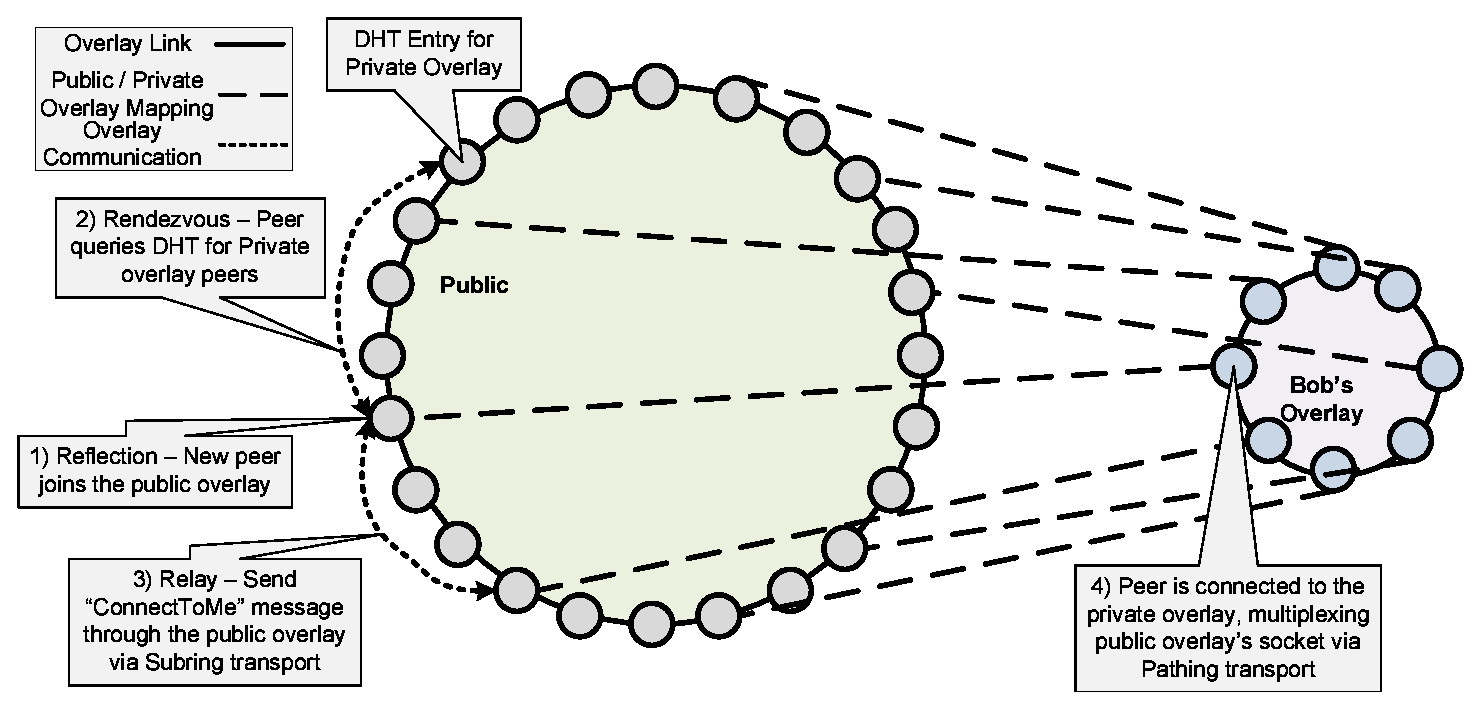
\epsfig{file=figs/bootstrap_brunet.eps, width=5.5in}
\caption{Bootstrapping a P2P system using Brunet.}
\label{fig:bootstrap_brunet}
\end{figure}
\end{center}

\subsection{Using XMPP}
\label{bs:xmpp_bootstrapping}

In addition to supporting recursive bootstrapping of private overlays, the
techniques described above can be extended to use a different public overlay,
an XMPP-based federation, to support the bootstrapping of private overlays.
The key features that make XMPP attractive are the distributed nature of the
federation and the openness of the protocol.  As of December 2009, there are
over 70 active XMPP servers in the XMPP Federation~\cite{xmpp_servers}.  These
include GoogleTalk, Jabber.org, and Live Journal Talk.

In XMPP, each user has a unique identifier of the form ``username@domain''.
Where the domain specifies the client's XMPP server and the username uniquely
identifies a single individual.  XMPP supports concurrent instances for each
user by appending a resource identifier to the user ID:
``username@domain/resource''.  A resource identifier can either be provided by
the client or generated by the server.  For users in the same domain, the
server forwards the message from source to destination.  When two users are in
different domains, the sender's server forwards the message to the receiver's
server, who then relays it to the receiver.

XMMP allows for sending arbitrary binary messages called ``IQ''.  While peer
relationships are maintained by the server, they are initiated between peers
using ``IQ''.  Once peers have established a connection or subscription, they
are informed through a ``Presence'' notification that the peer has come online,
this include the full user identifier.

The first form of \textbf{reflection} in XMPP is the unique client identifier.
Another is an IP reflection service available from some XMPP service providers
called ``Jingle''~\cite{jingle}.  ``Jingle'' uses ``IQ'' to determine available
STUN and TURN servers.  Fortunately, these services are provided free of charge
through GoogleTalk.  In Brunet, I extended the UDP transport to support
querying STUN servers to obtain and maintain and open an address mapping.  STUN
packets are easily distinguished from other packes as the first two bits are
set to 0 as well as a static cookie found in all messages.

In order to support the situation where two peers are unable to communicate
through the exchanged addresses, I have extended XMPP ``IQ'' as a transport to
support \textbf{relaying}.  Once peers has formed a connection through XMPP,
they are able to route connection information to each other and attempt to form
a direct connection.  In the case that this is unsuccessful, they are able to
fall back to this link as a means to transmit P2P data.  This approach also has
the benefit that, if a XMPP server does not support ``Jingle'', the two peers
can still form links with each other.  Since Brunet internally supports IP
reflection, eventually, if one of the peers in the system has a public address,
it will automatically assist the other peers into forming direct links with
each other.

\textbf{Rendezvous} uses a two step approach.  First peers advertise their use
of private overlay in the resource identifier.  The name is hashed to ensure
that the users complete identifier does not extend past 1,023 bytes, the
maximum length for these identifiers.  In addition, a cryptographically
generated random number is appended to the resource identifier to distinguish
between multiple instances of the users application in the same private
overlay.  Once a peer receives a presence notification from a remote peer and
the base components match, that is the hash of the service, the peer adds it to
a list of known online peers.  If the peer lacks connections, the system
broadcasts to that list a request for addresses.  The peers respond with a list
of addresses including UDP, TCP, and XMPP addresses, concluding rendezvous.

Ideally, peers would not need to create XMPP connections with each other; if
they are on a public address, the rendezvous phase alone will suffice.  When
peers do not have a public address, they can obtain a mapping through STUN,
then form an XMPP connection with each other, and finally perform simultaneous
connection attempts.  If NAT traversal fails, the peers can continue routing
through the XMPP connection.  Due to the abstractions employed by the transport
library, the additional support for XMPP-based bootstrapping required only an
additional 700 lines of code to Brunet and no modification to the core system.

\section{Evaluating Overlay Bootstrapping}
\label{bs:evaluations}

This section presents a qualitative evaluation of this system prototype
bootstrapping a small-scale network as well as some of the experiences in
deploying bootstrapping overlays.

\subsection{Deployment Experiments}

These experiments verify that the techniques work and determine expected
overheads in using Brunet and XMPP to bootstrap an overlay.  Rather than an
extensive experiment overly focused on overheads of Brunet and XMPP, this
experiment is primarily focused on the feasibility of forming small-scale
overlays among network-constrained peers.  The experiment represents 5 peers
desiring all-to-all direct connectivity, a feature transparently available to
them if they bootstrap into a private Brunet overlay. The experiments were run
on peers deployed on 5 distinct virtual machines.  Each virtual machine had its
own separate NAT, and thus peers were unable to communicate directly without
assistance.

The public Brunet overlay used in this experiment consisted of over 600 nodes
running on PlanetLab.  PlanetLab~\cite{planetlab} is a consortium of research
institutes sharing hundreds of globally distributed network and computing
resources.  GoogleTalk provided the XMPP overlay used in this experiment.
Though this experiment does not take into advantage the features of the XMPP
Federation, this aspect is presented in more detail in the next section
reviewing experiences deploying overlays using XMPP.

In the experiment, 5 P2P nodes were started simultaneously, while measuring the
time spent for reflection, rendezvous, reflection, and connection.  The results
are presented in Table~\ref{tab:results}.  For XMPP, these are translated as
follows:  reflection measures the time to obtain IP addresses from the STUN
server, rendezvous is the time to receive a presence notification, relaying is
the time to receive a message across XMPP, and connected is once all nodes in
the private overlay has all-to-all connectivity.  For Brunet, these are
translated as follows:  reflection measures the time to connect to the public
overlay, rendezvous is the time to query the DHT, relaying is the average time
to send a message across the overlay, and connected is the time until the
private overlay has all-to-all connectivity.  The results are highly correlated
to timeouts in Brunet, which employs a mixture of events and polling to
stabilize the overlay, as well as the latency between the client and
GoogleTalk.  As this was more of a qualitative experiment, the results are
clear: private overlays providing all-to-all connectivity among NATed nodes can
bootstrap within a very reasonable amount of time.

\begin{center}
\begin{table}
\caption{Time in seconds for various private overlay operations}
\begin{tabular*}{\textwidth}{@{\extracolsep{\fill}}
l
S[table-format=1.3,table-number-alignment=right]
S[table-format=1.3,table-number-alignment=right]
S[table-format=1.3,table-number-alignment=right]
S[table-format=2.2,table-number-alignment=right]
@{}
}

\hline & 
\multicolumn{1}{c}{Reflection} &
\multicolumn{1}{c}{Rendezvous} &
\multicolumn{1}{c}{Relaying} &
\multicolumn{1}{c}{Connected} \\ \hline \hline
XMPP & .035 & .110 & .243 & 20.3 \\ \hline
Brunet & 3.05 & .330 & .533 & 23.22 \\ \hline
\end{tabular*}
\label{tab:results}
\end{table}
\end{center}

\subsection{Deployment Experiences}

Recently, Facebook announced that they would be supporting XMPP as a means to
connect to Facebook chat.  This was rather exciting and further motivated this
work, as Facebook has over 400 million active users, which would have made
their XMPP overlay, potentially, the largest free-to-join overlay.
Unfortunately, Facebook does not employ a traditional XMPP setup, instead it
provides a proxy into their chat network, preventing features like arbitrary
IQs and other forms of out-of-band messages to be exchanged between peers.
User identifiers are also translated, so a peer cannot obtain a remote peers
real identifier.  Thus there exists no out-of-band mechanism for rendezvous.
Peers could potentially send rendezvous messages through the in-band XMPP
messaging, but this may be viewed by most recipients as spam as it would arrive
as normal chat messages.  Unfortunately, the realization is that not all XMMP
servers, especially those unrelated to the Federation, support features
necessary to bootstrap.

During initial tests in verifying the workings of the XMPP code base, I
bootstrapped a private Brunet overlay on PlanetLab through various XMPP service
providers.  Unfortunately, some servers (GoogleTalk) ignored clients on
PlanetLab.  Another server crashed after 257 concurrent instances of the same
account logged in.  Because the provider had no contact information, I was
unable to ascertain the reason for the crash.  Though there did exist some
servers that had no trouble hosting over 600 concurrent instances running on
PlanetLab.

Once the system was running on PlanetLab, more tests were performed to
determine the ability to bootstrap across the XMPP Federation.  For this
purpose, several friendships, or subscriptions, were formed between users
across various XMPP service providers.  In the most evaluated case, a single
peer on GoogleTalk along with 600 peers on PlanetLab system using
\textit{jabber.rootbash.com}, the GoogleTalk peer would not always receive
presence notifications for all peers online, though always would receive some.
When a peer began the relaying mechanism, it would broadcast to every peer from
whom it received a presence notification.  When performing this between
GoogleTalk and \textit{rootbash}, the GoogleTalk peer would not receive a
response.  Though in reducing the broadcast to a random selection of 10 peers,
every 10 seconds until the GoogleTalk peer was connected, the peer received
responses.  The behavior indicates that the XMPP servers may have been
filtering to prevent denial of service attacks.

Peers on the same XMPP server seem to be connected very quickly, though peers
on different services can take significantly longer.  For example, when
bootstrapping a single peer from GoogleTalk into the \textit{rootbash} system,
it always took 1 minute for the node to become fully connected to the private
overlay.  When the peer used \textit{rootbash}, the peer always connected
within 30 seconds.  It seems as if the communication between XMPP servers was
being delayed for some reason.  The same behavior was not experienced, when
chatting between the two peers.

\begin{center}
\singlespacing{
\footnotesize{
\begin{longtable}{p{.85in}p{1.5in}p{1.2in}p{1.05in}p{1.05in}}

\caption[Public and research overlays]{Public and research overlays} \\

\hline & Description & Reflection & Rendezvous & Relay \\ \hline
\endfirsthead

\multicolumn{5}{l}{\normalsize{Table \ref{tab:overlays}. Continued}}\\
\hline & Description & Reflection & Rendezvous & Relay \\ \hline
\endhead

\hline
BitTorrent &
Default BitTorrent implementations rely on a centralized tracker to provide the
initial bootstrapping.  Peers can establish new connections through information
obtained from established connections.  This relegates the tracker as a means
of monitoring the state of the file distribution.  BitTorrent specifies a
protocol, though each client may support additional features not covered by the
protocol.
&
The current specification does not support NAT traversal, though future
versions may potentially use UDP NAT traversal.  At which point, BitTorrent may
support a reflection service.
&
Peers can register as seeds to the same file hash, thus their IP address will
be stored with the tracker.
&
Peers receive each other's IP addresses from the tracker, there is no inherent
relaying.
\\ \hline
Gnutella &
Gnutella is a large-scale unstructured overlay with over a million peers;
primarily, it is used for file sharing.  Gnutella consists of a couple
hundred thousand ultra (super) peers to provide reliability to the overlay.
Gnutella is free-to-join and requires no registration to use.
&
Work in progress.  Peers attempt to connect to a sharer's resource, though a
"Push" notification reverses this behavior.  Thus a peer behind a NAT can
share with a peer on a public address.
&
Peers can perform broadcast searches with TTL up to 2; when networks consist of
millions of peers, small overlays will most likely not be able to discover each
other.
&
Not explicitly, could potentially utilize ping messages to exchange messages.
\\ \hline
Skype &
Skype is a large-scale unstructured overlay, consisting of over a million
active peers, and primarily used for voice over P2P communication.  Skype, like
Gnutella, also has super peers, though the owners of Skype provide
authentication and bootstrap servers.  Though Skype is free-to-join, it
requires registration to use.
&
Skype APIs provide no means for reflection.
&
Skype supports applications, or add-ons, which can used to transparently
broadcast queries to a users friend to determine if the peer has the
application installed.  Thus Skype does support rendezvous.
&
Skype applications are allowed to route messages via the Skype overlay, but
because Skype lacks reflection, all communication must traverse the Skype
overlay.
\\ \hline
XMPP &
XMPP consists of a federation of distributed servers.  Peers must register an
account with a server, though registration can be done through XMPP APIs without
user interaction.  XMPP is not a traditional P2P system, though it has some P2P
features.  XMPP servers on distinct servers are able to communicate with each
other.  Links between servers are created based upon client demand.  During link
creation, servers exchange XMPP Federation signed certificates.
&
While not provided by all XMPP servers, there exist extensions for NAT
traversal.  GoogleTalk, for example, provides both STUN and TURN servers.
&
Similar to Skype, XMPP friends can broadcast queries to each other to find
other peers using the same P2P service.  Thus XMPP supports rendezvous.
&
The XMPP specification allows peers to exchange arbitrary out-of-band
communication with each other.  Most servers support this behavior, even
when sent across the Federation.  Thus XMPP supports relaying.
\\ \hline
Kademlia~\cite{kademlia} &
There exists two popular Kademlia systems, one used by many BitTorrent systems,
Kad, and the other used by Gnutella, called Mojito.  Kademlia implements an
iterative structured overlays, where peers query each other directly when
searching the overlay.  Thus all resources of a Kademlia overlay must have
a publicly addressable network endpoint.
&
Existing implementations of Kademlia do not support mechanims for peers to
determine their network identity.
&
Peers can use the DHT as a rendezvous service, storing their connectivity
information in the DHT at key location:  $hash(SERVICE)$.
&
An iterative structured overlay has no support for relaying messages.
\\ \hline
OpenDHT~\cite{opendht} &
OpenDHT is a recently decommissioned DHT running on PlanetLab.  OpenDHT is
built using Bamboo, a Pastry-like protocol~\cite{pastry}.  Pastry implements
recursive routing, peers route messages through the overlay.
&
Existing implementations of Bamboo and Pastry do not support mechanims for
peers to determine their network identity.  Though this is ongoing work.
&
Peers can use the DHT as a rendezvous service, storing their connectivity
information in the DHT at key location:  $hash(SERVICE)$.
&
Because Pastry uses recursive routing, it can be used as a relay.  Furthermore,
extensions to Pastry have enabled explicit relays called virtual
connections~\cite{epost}.
\\ \hline
Brunet~\cite{brunet} &
Brunet like OpenDHT is a freely available DHT running on PlanetLab, though
still in active development.  Brunet creates a Symphony~\cite{symphony} overlay
using recursive routing.
&
Brunet supports inherent reflection services, when a peer forms a connection
with a remote peer, the peers exchange their view of each other.
&
Peers can use the DHT as a rendezvous service, storing their connectivity
information in the DHT at key location:  $hash(SERVICE)$.
&
Like Pastry, Brunet supports recursive routing and relays called
tunnels~\cite{hpdc08_0}.
\\ \hline
\label{tab:overlays}
\end{longtable}}}
\end{center}


\chapter{FROM OVERLAYS TO SECURE VIRTUAL PRIVATE NETWORKS}
\label{chap:security}

In this chapter, I take the results from Chapter~\ref{chap:bootstrapping} and
apply them to IPOP~\cite{ipop} in order to construct a fully decentralized P2P
VPN.  While sharing overlays in IPOP makes for simplified use of the system, in
reality, it introduces significant security challenges.  For example, a
misconfigured or malicious peer could potentially disable the entire overlay,
rendering all VNs useless.  If security and hence isolation is important, prior
to VN deployment, a user would need to deploy a secure overlay and configure
their VPN to bootstrap from it, given the complexity many users may reconsider
the P2P approach and use a simple centralized VPn.

To address this challenge and to make a fully decentralized P2P VPN, I have
extended the IPOP concept to support bootstrapping from public infrastructures
and overlays into private and secure P2P overlays whose membership is limited
to an individual VPN user base.  Chapter~\ref{chap:bootstrapping} focused on a
small scale feasibility of bootstrapping decentralized overlays.  This chapter
further extends into performance overheads of recursive Brunet overlays and
larger network sizes.  I then consider security in the overlay and present the
first implementation and evaluation of an overlay with secure communication
both between end points in the P2P overlay (e.g. VPN nodes) as well as between
nodes connected by overlay edges.  Security requires a means for peer
revocation; however, current revocation techniques rely on centralized systems
such as certificate revocation lists (CRLs). The proposed approach allows
revocation using scalable techniques provided by the P2P overlay itself.  I
call the completed system and the interface used to administrate it {\bf
GroupVPN}, a novel decentralized P2P VPN.

The rest of this chapter is organized as follows.  Throughout the chapter,
there are two techniques used to evaluate my approaches, simulation and real
system deployments; these are described in Section~\ref{vpn:experimental}.
Section~\ref{vpn:private_overlays} describes techniques that allow users to
create their own private overlays from a shared public overlay in spite of
NATs.  Use of security protocols has been assumed in many P2P works, though
without consideration of implementation and overheads. I investigate
implementation issues and overheads of security in P2P with emphasis on P2P
VPNs in Section~\ref{vpn:security}.  Without revocation, use of security is
limited, and in decentralized systems, the use of centralized revocation
methods is are not sufficient, I present novel mechanisms for decentralized
revocation in Section~\ref{vpn:revocation}.  The complete system, GroupVPN, is
presented in Section~\ref{vpn:groupvpn}.  Section~\ref{vpn:related_work}
compares and contrasts this work with related work.  

\section{Experimental Environment}
\label{vpn:experimental}

Throughout this paper, my quantitative evaluation environment uses both real
deployments on PlanetLab and simulation.  The evaluation requirements dictate
the environment used.  When the perspective of a single node is useful,
PlanetLab's overloaded nature makes complex system analysis challenging,
especially when attempting to simulate an instanteous behavior on a system,
which has random outage and delays in access.

IPOP uses Brunet as the underlying P2P infrastructure for connectivity.  Brunet
has been in active development for the past 5 years and is routinely run on
PlanetLab~\cite{planetlab} for experiments and tests.  PlanetLab consists of of
nearly 1,000 resources distributed across Earth.  In practical applications,
though, roughly 40\% of the resources are unavailable at any given time and the
remaining behave somewhat unpredictably.

PlanetLab deployment takes approximately 15 minutes for all resources to have
Brunet installed and connect to the overlay and then much more time to observe
certain behaviors, making regression and verification tests complicated.  To
address this, I have extended Brunet to support a simulation mode. The
simulator inherits all of the Brunet P2P overlay logic but uses simulated
virtual time based upon an event-driven scheduler instead of real time.
Furthermore, the simulation framework uses a specialized transport layer to
avoid the overhead of using TCP or UDP on the host system, both of which are
limited resources and can hamper the ability to simulate large systems.   The
specialized transport uses datagrams to pass messages between nodes, thus from
the node's perspective, it is very similar to a UDP transport and can simulate
both latency and packet dropping.  Latency between all node pairs is set to 100
ms by default.

Both simulation and real system evaluation provide unique advantages.
Simulations allow faster than real time execution of reasonable sized networks
(up to a few thousand) using a single resource, while enabling easy debugging.
In contrast, deployment on real systems, in particular PlanetLab, presents
opportunities to add non-deterministic, dynamic behavior into the system which
can be difficult to replicate, such as network glitches and long CPU delays on
processing.

\section{Towards Private Overlays}
\label{vpn:private_overlays}

Many users of IPOP begin by using the public shared overlay and, once
comfortable, move towards hosting their own infrastructure.  Some are
successful without assistance, while a majority are not.  Network configuration
issues tend to be the most common issue preventing users from hosting their own
independent IPOP systems.  While users were able to easily join the shared
overlay, similar attempts to construct their own were hindered and ultimately
only successful after receiving feedback.

Prior work in IPOP~\cite{pcgrid07} enabled many VPNs to share a single P2P
overlay by storing IP address into the DHT at the key $hash(Namespace:IP)$.
Unfortunately, this approach is fraught with security issues.  In the previous
chapter, I established methods that enabled bootstrapping private Brunet
overlays as easily as connecting to a public P2P overlay.  This chapter begins
by focusing on the integration of the methodologies employed in recursive
Brunet overlays as applied to IPOP.

To bootstrap from an existing Brunet overlay, peers first insert their public
overlay node address into the key represented by $hash(\$Private Overlay
Namespace)$ and continue to do so regularly until they disconnect, so as to not
let the entry become stale and disappear.  Peers attempting to bootstrap into
the private overlay can then query this key and obtain a list of public overlay
nodes that are currently acting as proxies into the private overlay.  By using
the public overlay as a transport, similar to UDP or TCP, the private overlay
node forms bootstrapping connections via the public overlay.  At which point,
overlay bootstrapping proceeds as normal.  The entire process is represented in
Figure~\ref{fig:bootstrap}.

As mentioned in the previous chapter, small overlays may have no members with a
public address, making it difficult to provide overlay based NAT traversal.  To
avoid having a special case for NAT traversal in private overlays, in my model,
the private overlay share TCP and UDP sockets with the public overlay.  This
mechanism, referred to as {\em ``pathing''}, allows multiplexing a single UDP
socket and listening TCP socket by many overlays.  This is only possible due to
the generic transports library of the Brunet P2P overlay, which does not
differentiate UDP, TCP, or even relayed links.  Pathing works as a proxy,
intercepting a link creation request from a local entity, mapping that to a
path, and then requesting from the remote entity a link for that path.  The
underlying link is then wrapped by pathing and given to the correct overlay
node, resulting in a completely transparent multiplexing of a TCP and UDP
sockets, thereby enabling the NAT traversal in one overlay to benefit the
other.  Once a link has been established, the pathing information is
irrelevant, limiting the overhead into the system to a single message exchange
during link establishment.

\subsection{Time to Bootstrap a Private Overlay}

This experiment focuses on the overheads in bootstrapping a private overlay
using the techniques mentioned in the previous section.  The time to bootstrap
can be derived analytically by considering the minimum steps for a node to join
the public overlay, obtain private overlay peers from the public overlay DHT,
and then connect to the private overlay.  In Brunet, peers begin by forming
leaf or bootstrapping connections and use these to communicate with the
neighbor or peer in the P2P network nearest to their P2P address.  The process
to form a connection can be done in as few as 4 messages and up to 6, if the
peers only know each other's P2P address, which is the case for neighbor
connections.

Assuming a peer already has IP address information for another, a connection
can be initiated by the peer sending a message to the remote peer expressing
the desire for a connection.  The remote node responds by either rejecting the
request or committing to the connection.  In the next exchange, the initiating
peer commits to forming the connection and the remote peer acknowledges.  The
two phase commit process is used to handle the complexity that ensues when
multiple simultaneous connection attempts occur in parallel.  All these
messages take $1$ hop, since they are direct links between peers.

When peers only have each other's P2P address and/or the initiating peer is
behind a NAT, it may take fifth and sometimes a sixth message.  These messages
are requests for the remote peer's IP addresses as well as asking the peer to
connect with the initiating peer, addressing the case where the remote peer is
behind a NAT and cannot handle inbound messages.  These messages are routed
over the overlay taking $\log(N)$ hops, where $N$ is the network size of the
public overlay.

Private overlay bootstrapping follows a similar process, though, first, the
peer acquires P2P addresses of other participants through the public DHT, an
operation taking $2 *\log(N)$ hops.  In the private overlay, the leaf
connections do not communicate directly; rather, they use the public overlay,
causing some of the $1$ hop operations above to take $\log(N)$ hops.  Finally,
finding the nearest remote peer in the private overlay takes $\log(N) +
\log(n)$, where $n$ is the network size of the private overlay.

Given this model, each operation takes the following hop counts: public overlay
bootstrapping $=>$ $8 + \log(N)$, DHT operations $=>$ $2 * \log(N)$, and
private overlay bootstrapping $=>$ $4 + 5 * \log(N) + \log(n)$.  The cumulative
operation takes $12 + 8 * \log(N) + \log(n)$ hops.  The dominating overhead in
bootstrapping the private overlay is the time it takes to perform overlay
operations on the public overlay ($\log(N)$).  For instance, assuming a network
size of 512 public and 8 private, a node should be connected within 87 hops.

To evaluate my implementation for GroupVPN, I used both PlanetLab and the
simulator.  100 tests were run for various network sizes.  Though due to
difficulty in controlling network sizes in PlanetLab, I set each PlanetLab node
to randomly decide if it would connect to the private overlay.  The network
sizes were then used in the simulator and the analytical model.  The average
public network size for each of these tests was 600.  The results are presented
in Figure~\ref{fig:private_bootstrapping}~\footnote{I performed measurements
for many more private network sizes, but all the results were so similar that
it did not introduce anything of interest and are omitted from the  plots to
improve clarity.}.

\begin{figure}[ht]
\centering
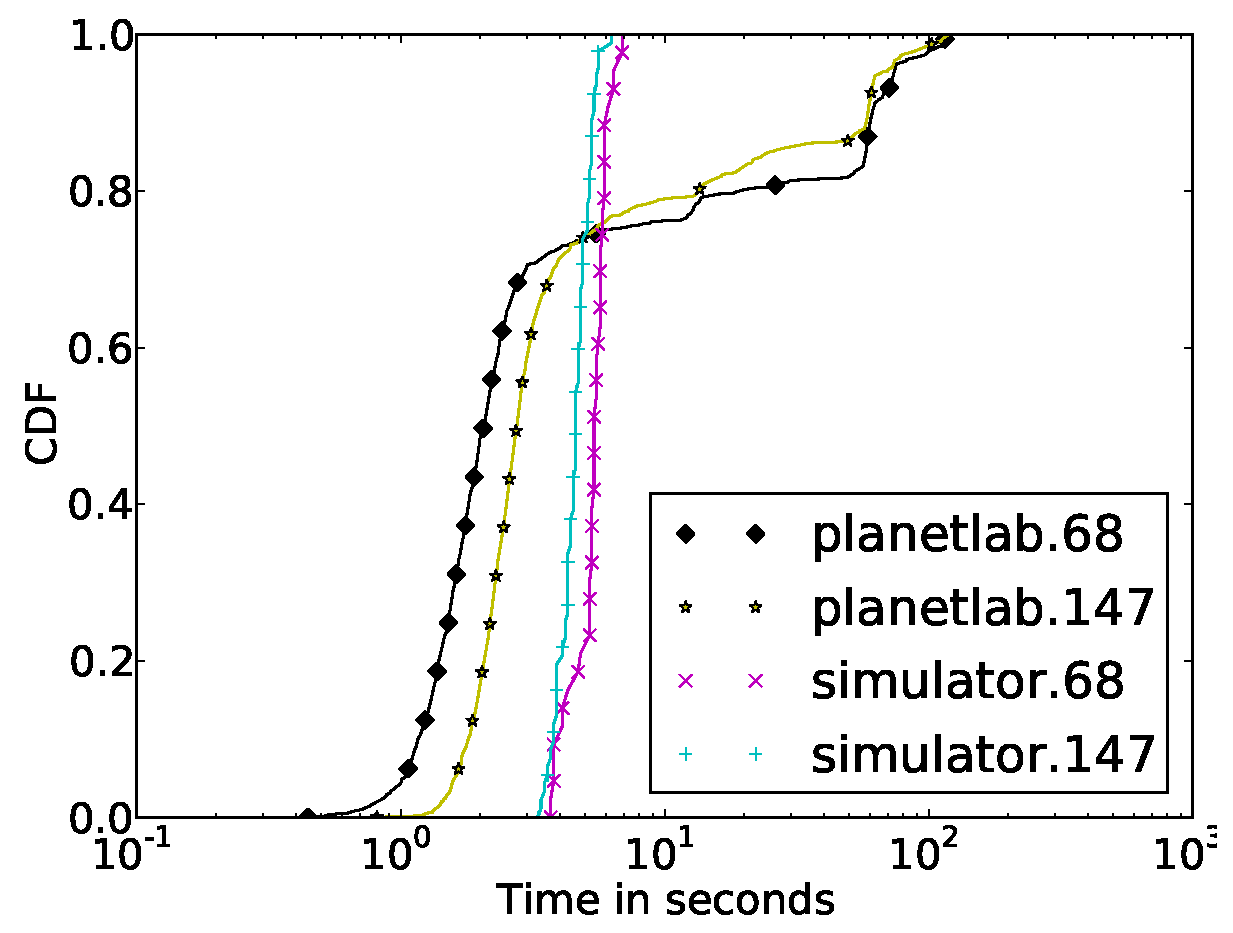
\includegraphics[width=4in]{figs/private.eps}
\caption[CDF of private overlay bootstrap time]{CDF of the time to bootstrap a
private overlay node in a private overlay of the size stated in the legend
using a public overlay consisting of 600 nodes.  Using a 100 ms delay like the
simulator results in 9.2 and 9.3 seconds for the analytical model for private
network sizes of 68 and 147, respectively.}
\label{fig:private_bootstrapping}
\end{figure}

Based upon the results presented in Figure~\ref{fig:private_bootstrapping}, the
bootstrapping time for the implementation performs better than the analytical
model, due to the simplicity of the analytical model and the small network
sizes.  It is of interest that while the simulator results tend to be in a well
defined range, the PlanetLab results have a few outliers with long bootstrap
times.  Some of the expected causes for this are churn in the system and state
machine timeouts in Brunet, though I have not considered this in much depth.

\subsection{Overhead of Pathing}

Much like the previous experiment, this verifies that the pathing technique has
negligible overheads for VPN usage.  To determine the overheads, two GroupVPNs
are deployed on resources on the same gigabit LAN.  To measure latency and
throughput, netperf experiments are run for 30 seconds, 5 times each on an
unutilized network switch.  Other specifications of the machine are ignored as
the system without pathing is used as the baseline.  The results,
Table~\ref{tab:pathing}, indicate that the use of pathing presents negligible
overhead for both throughput and latency, justifying the use of this approach
to transparently deal with NAT and firewall traversal.

\begin{table}[ht]
\caption[Pathing overheads]{Pathing overheads}
\centering
\begin{tabular*}{\textwidth}{@{\extracolsep{\fill}}
l
S[table-format=1.3,table-number-alignment=right]
S[table-format=3.2,table-number-alignment=right]
@{}
}
\hline & 
\multicolumn{1}{c}{Latency (ms)} &
\multicolumn{1}{c}{Throughput (Mbit/s)} \\ \hline \hline
Standard & .303 & 225.27 \\ \hline
Pathing & .308 & 224.36 \\ \hline
\end{tabular*}
\label{tab:pathing}
\end{table}

\section{Security for the Overlay and the VPN}
\label{vpn:security}

Structured overlays are difficult to secure and a private overlay is not secure
if it provides no means to limit access to the system.  Malicious users can
pollute the DHT, send bogus messages, and even prevent the overlay from
functioning, rendering the VPN useless.  To address this in means that make
sense for VPNs and common users, I have employed a public key infrastructure
(PKI) to encrypt and authenticate both communication between peers as well as
communication across the overlay, called point-to-point (PtP) and end-to-end
(EtE) communication, respectively.

Use of a PKI motivates from the ability to authenticate without a third party,
ideal for P2P use, unlike a key distribution centers (KDC) used by other VPNs.
A PKI can use either pre-exchange public keys or a certificate authority (CA)
to sign public keys, i.e., certificates.  Thus peers can exchange keys and
certificates without requiring a third-party to be online.

The reasons for securing PtP and EtE are different.  Securing PtP communication
prevents unauthorized access to the overlay, as peers must authenticate with
each other for every link created.  Though once authenticated, a peer can
perform malicious acts and since the overlay allows for routing over it, the
peer can disguise the origination of the malicious acts.  By also employing EtE
security, the authenticity of messages transferred through an overlay can be
verified.  Though EtE security by itself, will not prevent unauthorized access
into the overlay.  By employing both PtP and EtE, overlays can be secured from
uninvited guests from the outside and can identify malicious users on the
inside.  Implementing both leads to important questions: what mechanisms can be
used to implement both and what are the effects of both on an overlay and to a
VPN on an overlay.

\subsection{Implementing Overlay Security}

There are various types of PtP links, such as TCP and UDP sockets and relays
across individual nodes and the overlay.  EtE communication is
datagram-oriented in IPOP.  Traditional approaches of securing communication
such as IPsec are not convenient due to complexity, i.e., operating system
specific, portability constraints, and lack of common APIs.  Security protocols
that rely on reliable connections, such as SSL or TLS are undesirable as well
as they would require a userspace implementation of reliable streams (akin to
TCP).  As such, I have implemented an abstraction called a security filter as
presented in Figure~\ref{fig:security_filter}, which enables nearly transparent
use of security libraries and protocols.  To this date, I have implemented both
a DTLS~\cite{dtls} filter using the OpenSSL implementation of DTLS as well as a
protocol that reuses cryptographic libraries provided by .NET that behaves
similarly to IPsec.

A security filter has two components: the manager, and individual sessions or
filters.  While the individual sessions could act as filters by themselves, by
combining with a manager, they can be configured for a common purpose and
security credentials.  This approach enables the use of security to be
transparent to the other components of the system as the manager handles
session establishment, garbage collection of expired sessions, and revocation
of peers.

\begin{figure}
\centering
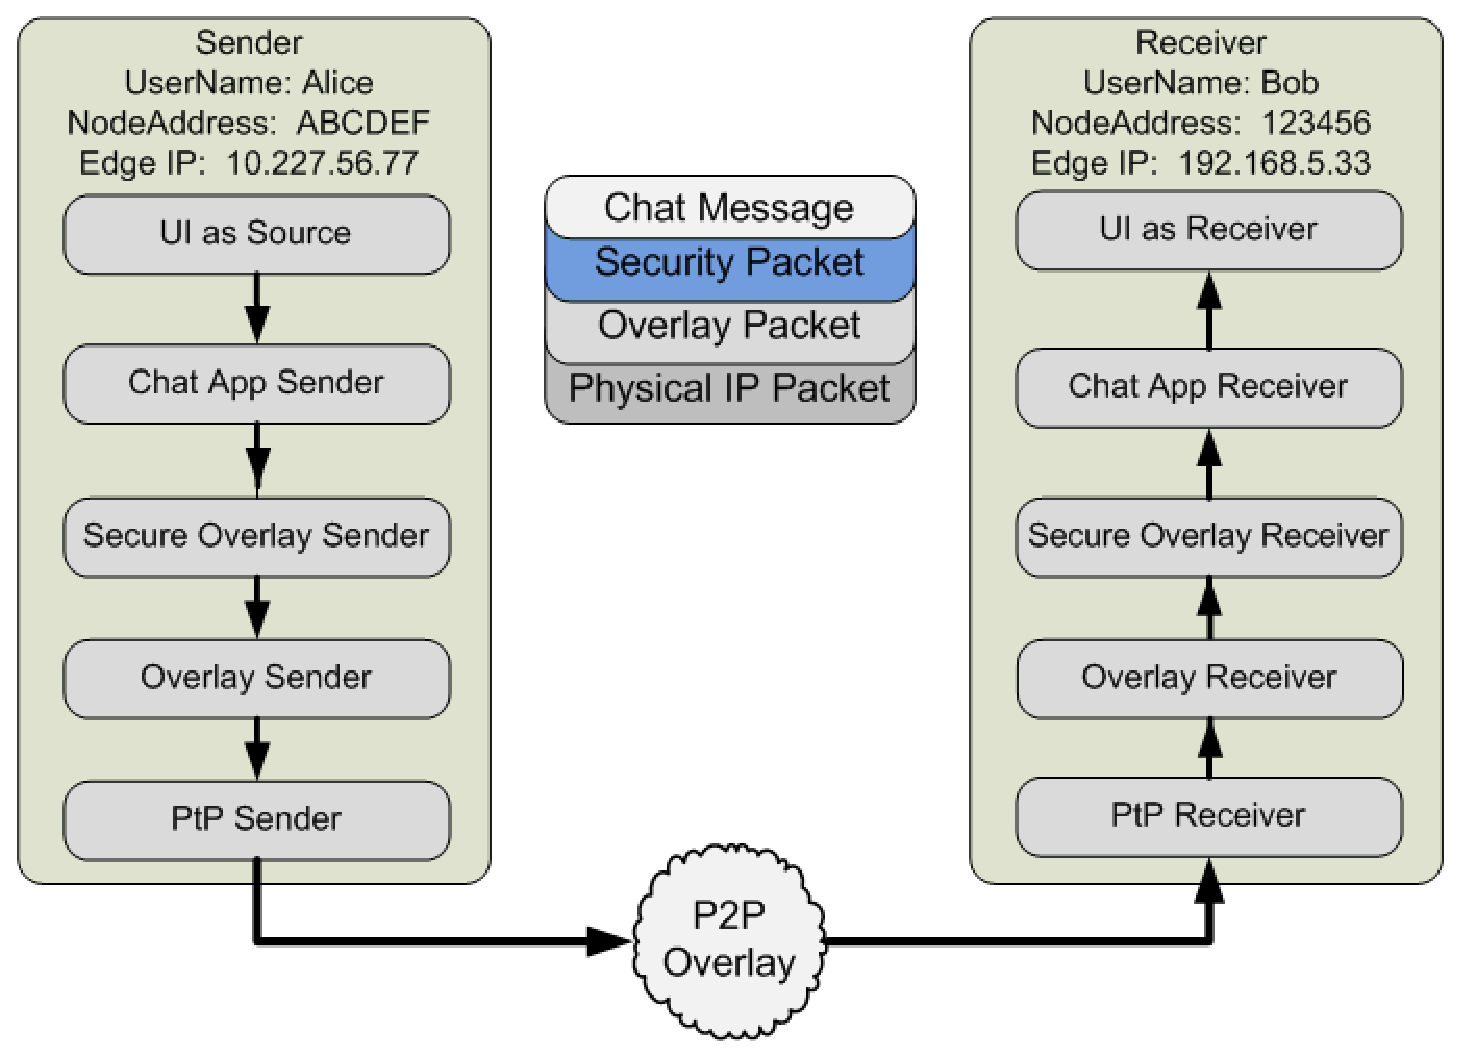
\includegraphics[width=6in]{figs/secure_sender_stack_generic.png.eps}
\caption[Security filter]{An example of the security filter abstraction used by
senders and receivers through an EtE secured chat application.  Each receiver
and sender use the same abstracted model and thus the chat application requires
only high-level changes, such as verifying the certificate used is Alice's and
Bob's, to support security.}
\label{fig:security_filter}
\end{figure}

Certificate embed identity of the owner, thus a signed certificate states that
the signer trusts that the identity is accurate.  In network systems, the
certificate uses the domain name to uniquely identify and limit the use of a
certificate.  When a CA signs the certificate, by including the domain name, it
ensures that users can trust that a certificate is valid, while used to secure
traffic to that domain.  Communication with another domain using the same
certificate will raise a flag and will result in the user not trusting the
certificate.  In environments with NATs, dynamic IP addresses, or portable
devices, typical of P2P systems, assigning a certificate to a domain name will
be a hassle as it constrains mobility and the type of users in the system.
Furthermore, most users are unaware of their IP address and changes to it.
Instead, a certificate is signed against the user's P2P address and unique user
name as delegated by the CA.  The purpose of the former is for efficiency of
revocation as discussed in Section~\ref{vpn:revocation}.  During the formation
of PtP links or while parsing EtE messages, the two nodes discover each other's
P2P addresses.  If the addresses do not match the address on the verified
certificate, the communication need not proceed further.  

Prior to trusting the security filter, the core software or the security filter
must ensure that the P2P address of the remote entity matches that of the
certificate.  In my approach, I did this by means of a callback, which presents
the underlying sending mechanism, EtE or PtP, and the overlay address stored in
the certificate.  The receiver of the callback can attempt to cast it into
known objects. If successful, it will compare the overlay address with the
sender type.  If unsuccessful, it ignores the request.  If any callbacks return
that the sender does not match the identifier, the session is immediately
closed.  Thus the security filter need not understand the sending mechanism and
the sending mechanism need not understand the security filter.

The last consideration comes in the case of EtE communication that provides an
abstraction layer.  For example, in the case of VPNs, where a P2P packet
contains an IP packet and thus a P2P address maps to a VPN IP address, a
malicious peer may establish a trusted link, but then hijack another user's IP
session.  As such, the application must verify that the IP address in the IP
packet matches the P2P address of the sender of the P2P packet.  In general, an
application address should be matched against a P2P address.

\subsection{Overheads of Overlay Security}

When applying an additional layer to a P2P system, there are overheads in terms
of time to connect with the overlay.  Other less obvious effects are
throughput, latency, and processing overheads, assuming that the P2P system
will be used over a wide area network, where the latency and throughput
limitations between two points will make the overhead of security negligible.
Though bootstrapping will be affected due to additional round trip messages
used for forming secure connections.

\begin{figure}[ht]
\centering
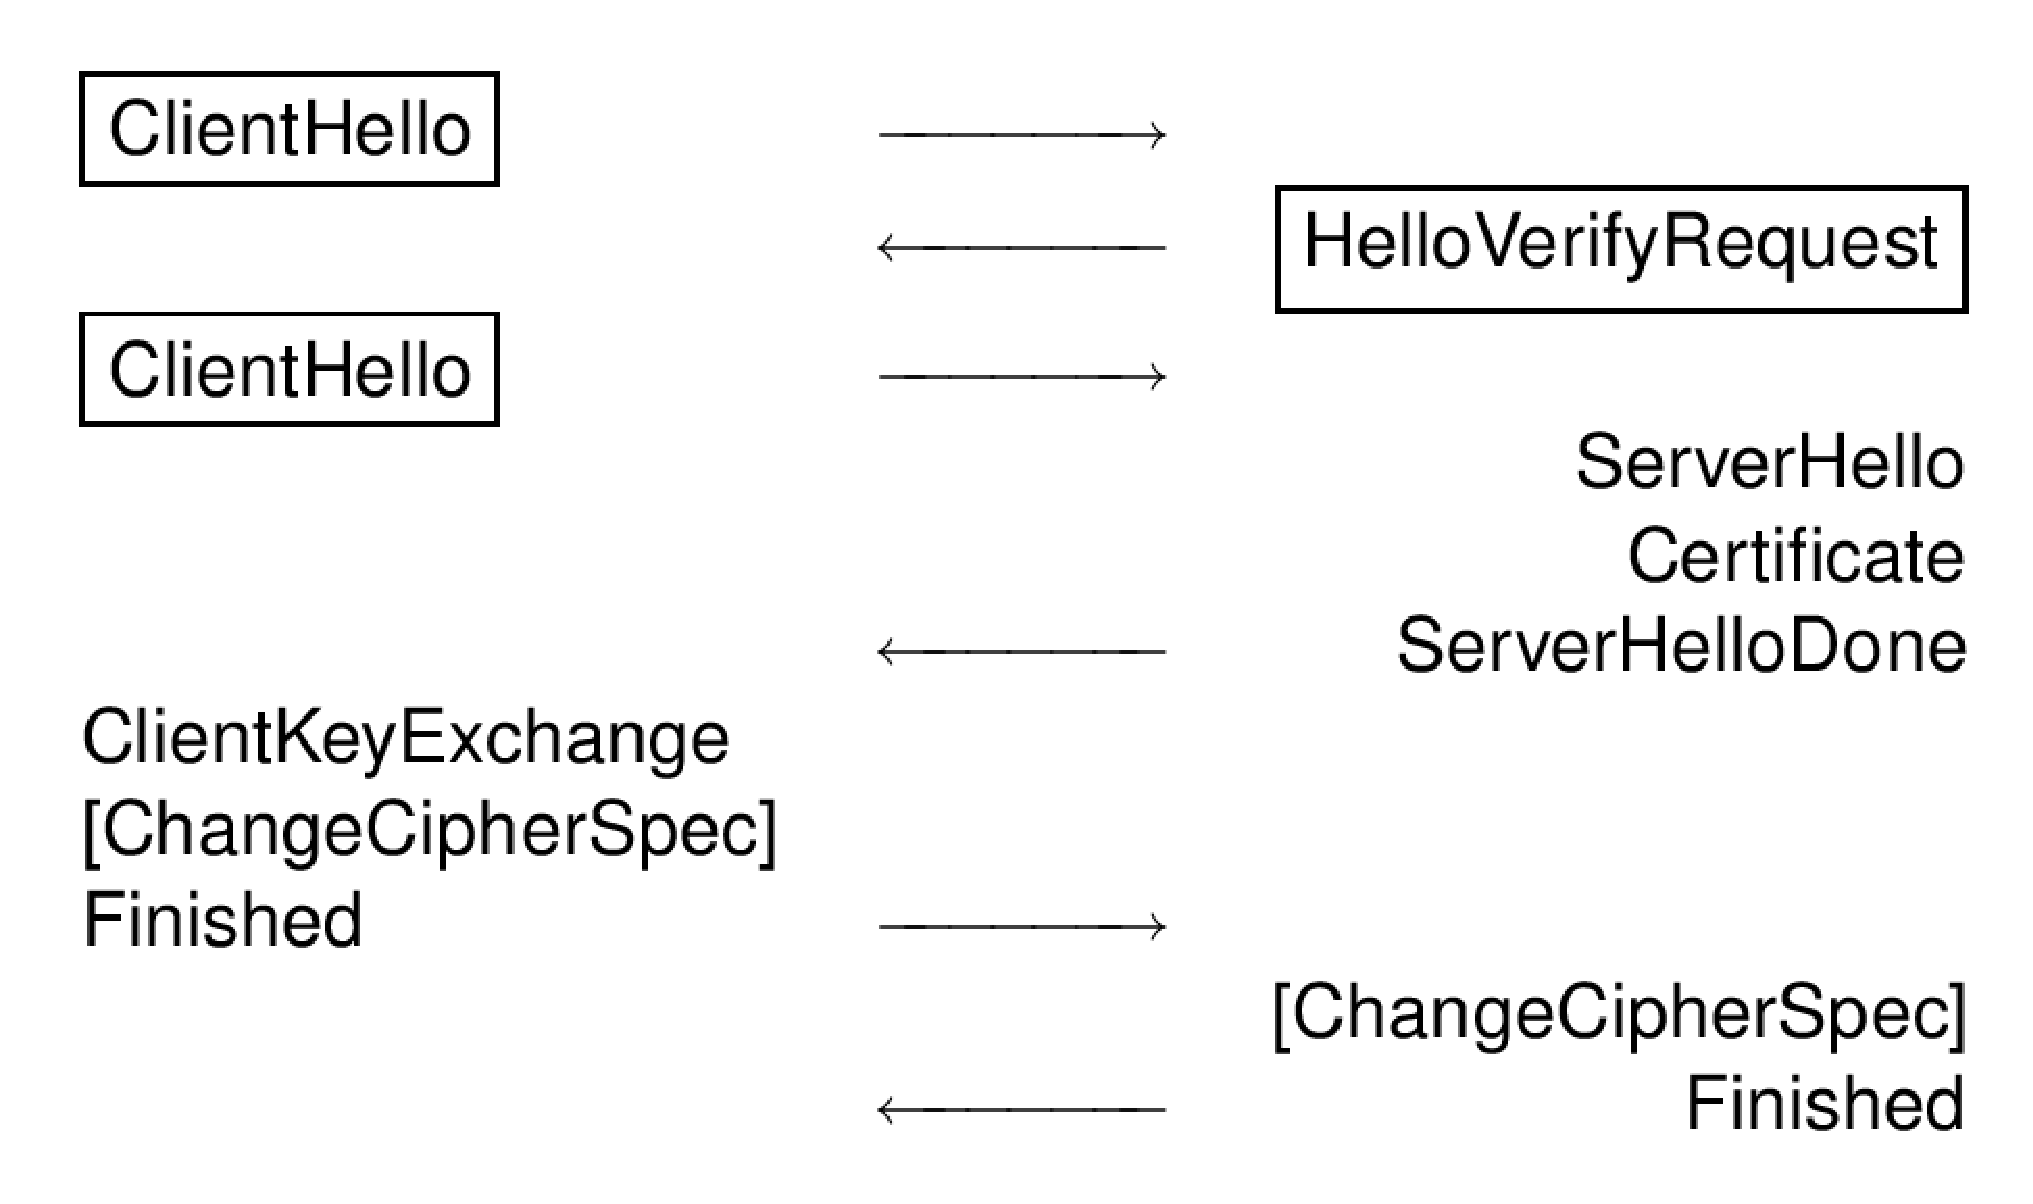
\includegraphics[width=4in]{figs/dtls.eps}
\caption[DTLS handshake]{DTLS handshake}
\label{fig:dtls}
\end{figure}

The DTLS handshake as presented in Figure~\ref{fig:dtls}, which consists of 6
messages or 3 round trips.  PtP security may very well have an effect on the
duration of overlay bootstrapping.  There even exists a possibility that with
more messages during bootstrap, the probability one drops is higher, which
could, in turn, also have an effect, though possibly negligible, on time to
connect.  To evaluate these concerns, I have employed both simulation and real
system experiments.

The following experiments use both simulation and PlanetLab deployment to
evaluate time to connect a new node to an existing resource.  Then another
experiment is performed to evaluate how long it takes to bootstrap various
sized overlays if all nodes join at the same time.  This experiment is only
feasible via simulation as attempting to reproduce in a real system is
extremely difficult due to how quickly the operations complete.

\subsubsection{Adding a Single Node}

This experiment determines how long it takes a single node to join an existing
overlay with and without DTLS security.  The experiment is performed using both
simulation and PlanetLab.  After deploying a set of nodes without security and
with security on PlanetLab, the network is crawled to determine the size of the
network.  In both cases, the overlay maintained an average size of around 600
nodes.  At which point, I connected a node 1,000, each time using a new,
randomly generated P2P address, thus connecting to a different point in the
overlay.  The experiment concludes as soon as the node has connected to the
peers in the P2P overlay immediately before and after it in the P2P address
space.  In the simulation, a new overlay is created and afterward a new node
joins, this is repeated 100 times.  The cumulative distribution functions
obtained from the different experiments are presented in
Figure~\ref{fig:add_one}.

\begin{figure}[ht]
\centering
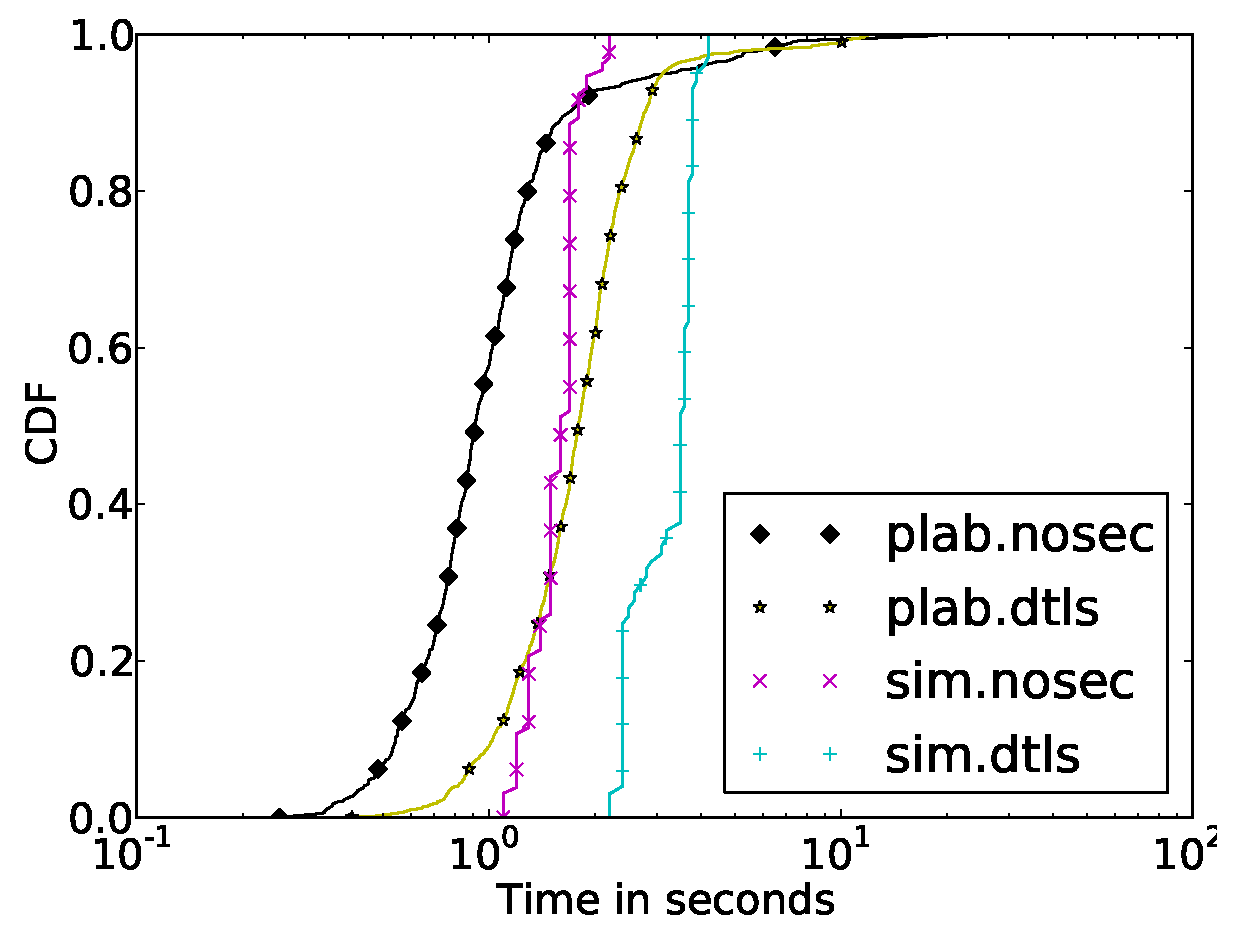
\includegraphics[width=4in]{figs/addone.eps}
\caption[Joining a secure overlay]{Time in seconds for a single node to join a
secure (dtls) and insecure (nosec) structured overlay, using both PlanetLab
(plab) and the Simulator (sim).} \label{fig:add_one}
\end{figure}

\subsubsection{Bootstrapping an Overlay}

The purpose of this experiment is to determine how quickly an overlay using
DTLS can bootstrap in comparison to one that does not given that there are no
existing participants.  Nodes in this evaluation are randomly given information
about 5 different nodes in the overlay and then all attempt to connect with
each other at the same time.  The evaluation completes after the entire overlay
has all nodes connected and in their proper position.  For each network size,
the test is performed 100 times and the average result is presented in
Figure~\ref{fig:bootstrap_eval}.

\begin{figure}[ht]
\centering
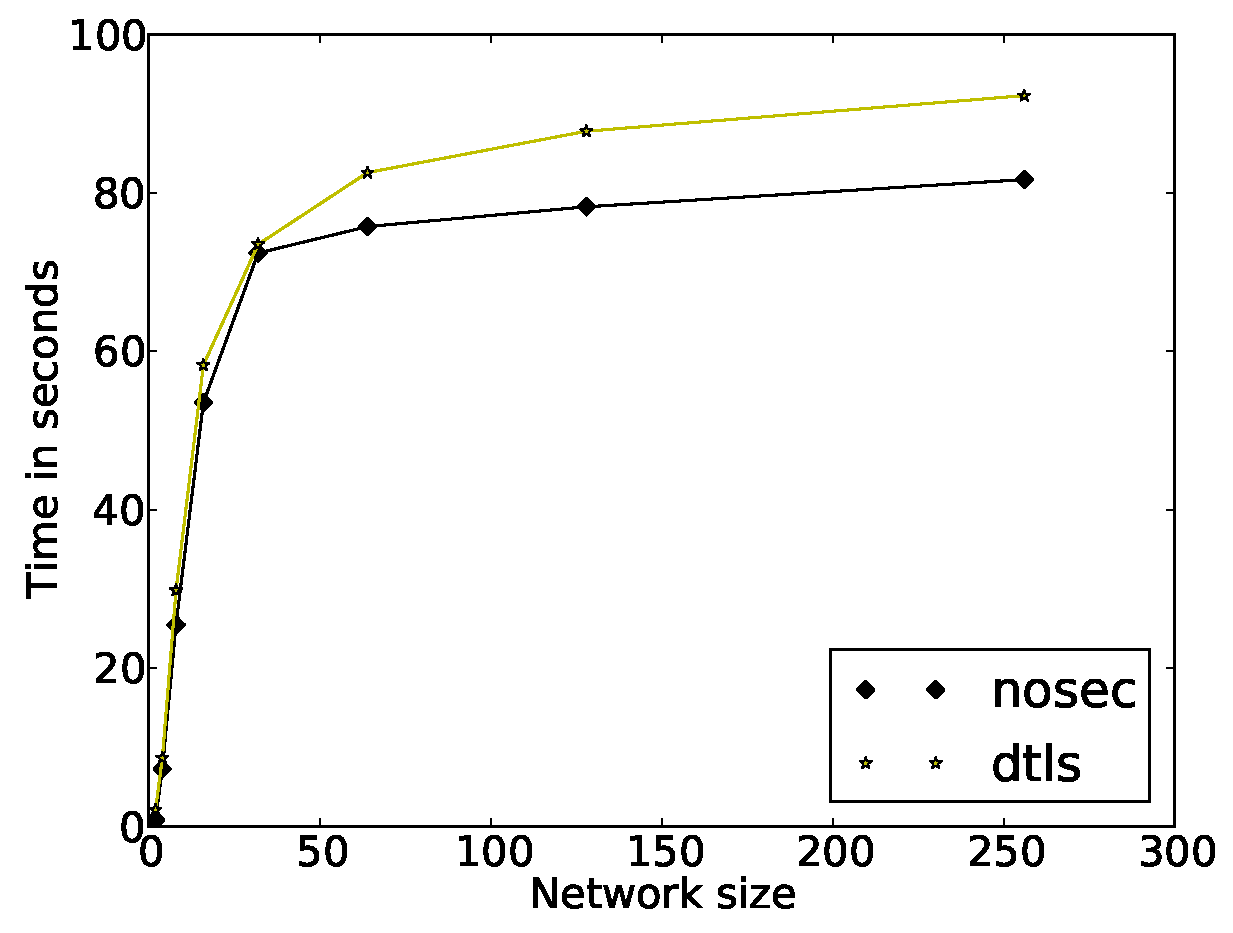
\includegraphics[width=4in]{figs/bootstrap_time.eps}
\caption[Bootstrapping a secure overlay]{Time in seconds for a secure (dtls)
and insecure (nosec) structured overlay to bootstrap, given that all nodes
bootstrap simultaneously.}
\label{fig:bootstrap_eval}
\end{figure}

\subsection{Discussion}

Both evaluations show that the overhead in using security is practically
negligible, when an overlay is small.  In the case of adding a single node, it
is clear that the simulation and deployment results agree, as the difference
between bootstrapping into an overlay with and without security remains nearly
the same.  Clearly this motivates the use of security if time to connect is the
most pressing question.

The time to bootstrap a secure overlay was not significantly more than that of
an insecure overlay.  What I realized is that complex connection handshaking,
as implemented in Brunet, seems to dominate connection establishment time.  For
example, in Brunet, two peers must communicate via the overlay prior to forming
a connection, and the system differentiates between bootstrapping connections
and overlay connections.  Thus even though a peer may have a bootstrapping
connection, it will need to go through the entire process to form an overlay
connection with a peer.  While this may lead to inefficiencies, this
simplification keeps the software more maintainable and easier to understand.

\section{Handling User Revocation}
\label{vpn:revocation}

Unlike decentralized systems that use shared secrets, in which the creator of
the overlay becomes powerless to control malicious users, PKIs enable their
creators to effectively remove malicious users.  Typical PKIs either use a
certificate revocation list (CRL) or online certificate verification protocols
such as Online Certificate Status Protocol (OCSP).  These approaches are
orthogonal to decentralized systems as they require a dedicated service
provider.  If the service provider is offline, an application can only rely on
historical information to make a decision on whether or not to trust a link.
In a decentralized system, these features can be enhanced so not to rely on a
single provider.  In this section, I present two mechanisms of doing so:
storing revocations in the DHT and performing overlay broadcast based
revocations.

\subsection{DHT Revocation}

A DHT can be used to provide revocation similar to that of OCSP or CRLs.
Revocations, a hash of the certificate and a time stamp signed by the CA, are
stored  are stored in the DHT at the key formed by the hashing of the
certificate.  In doing so, revocations will be uniformly distributed across the
overlay, not relying on any single entity.

The problem with the DHT approach is that it does not provide an event
notification for members currently communicating with the peer.  While peers
could continue to poll the DHT to determine a revocation, doing so is
inefficient.  Furthermore, a malicious peer, who has a valid but revoked
certificate could force every member in the overlay to query the DHT,
negatively affecting the DHT nodes storing the revocation.

\subsection{Broadcast Revocation}

Broadcast revocation uses a structured overlay based broadcast approach as
described in Appendix~\ref{broadcast}.  The form of broadcast can be used to
perform to notify the entire overlay immediately about a new revocation.  It is
important to note, that the message needs to be delivered locally prior to
forwarding, so that peers who have a connection to the malicious peer, will end
the connection prior to accidentally forwarding the message to the peer by
receiving and acting upon the revocation prior to forwarding the message.  

\subsection{Evaluation of Broadcast}

I performed an evaluation on the broadcast using the simulation to determine
how quickly peers in the overlay would receive the message.  The tested network
sizes ranged from 2 to 256 in powers of 2.  The tests were evaluations were
performed 100 times for each network size.  The CDF of hops for each node are
presented in Figure~\ref{fig:broadcast_cdf}.  The results make it quite clear that
the broadcast can efficiently distribute a revocation much more quickly than
$\log(N)$ time.

\begin{figure}[ht]
\centering
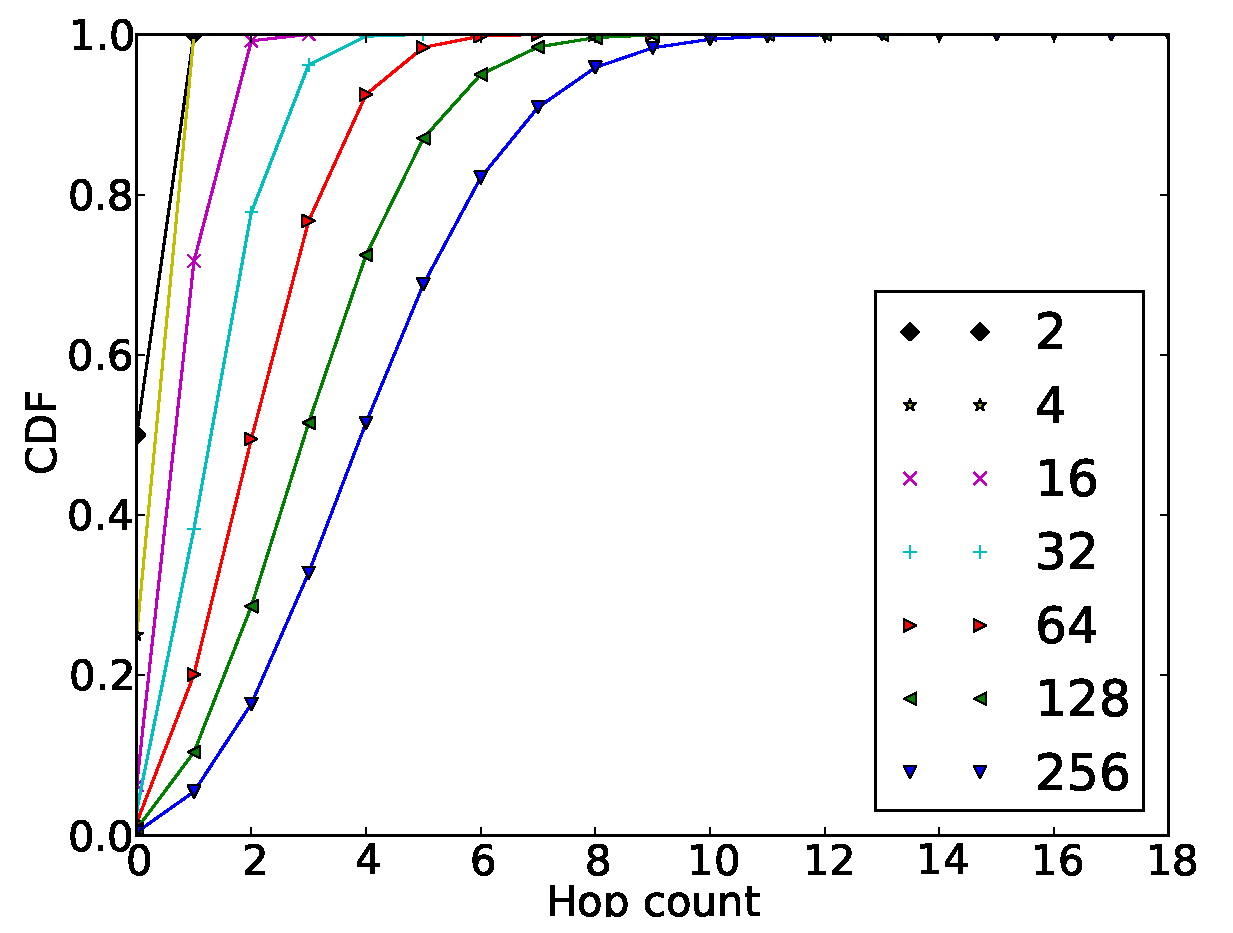
\includegraphics[width=4in]{figs/broadcast.eps}
\caption[Overlay broadcast time]{Overlay broadcast time CDF.}
\label{fig:broadcast_cdf}
\end{figure}

\subsection{Discussion}

In contrast to the DHT solution, broadcast revocation occurs only once and
leaves no state behind.  Thus the broadcast is not a complete solution, as new
peers connected to the overlay or those who missed the broadcast message will
be unaware of a revocation.  Furthermore, if an overlay is shared by many VPNs,
it may prevent overlay broadcasting or itself may be inefficient.

The DHT solution by itself may also not sufficient as revocations may be lost
over time as the entries must have their leases renewed in the DHT.  To address
this condition, each peer maintains a local CRL and the owner of the overlay
can occasionally send updates to the CRL through an out of band medium, such as
e-mail.  A better long term solution may be the use of a gossip protocols so
that peers can share their lists with each other during bootstrapping phases.

A key assumption in using these is that a Sybil~\cite{sybil}, or collusion
attack, is difficult in the secured overlay.	 If a Sybil attack is successful,
both a DHT and broadcast revocation may be unsuccessful, though peers could fix
this problem by obtaining the CRL out of band.  In addition, previous
work~\cite{secure_routing} has described decentralized techniques to limit the
probability of such attacks from occurring.  In my approach, the use of central
authority to review certificate requests can be used to limit a single user
from obtaining too many certificates as well as ensuring uniform distribution
of that user's P2P addresses, further hampering the likelihood of a Sybil
attack.  The ability to automate this is left as future work.

One way to mitigate sybil attacks using the broadcast approach is to bundle
colluding offenders into a single revocation message.  That would prevent those
from colluding together to prevent each other's revocations.  Furthermore,
while not emphasized above, revocation in my system revokes by user name and
not individual certificates.  Combined these two components limit Sybil attacks
against broadcast.

\section{Managing and Configuring the VPN}
\label{vpn:groupvpn}

While the PKI model applies to P2P overlays, actual deployment and maintenance
of security credentials can be too complex to manage, particularly for
non-experts.  Most PKI-enabled systems require the use of command-line
utilities and lack methods for assisting in the deployment of certificates and
policing users.  My solution to facilitate use of PKIs for non-experts is a
partially-automated PKI reliant on a group-based Web interface distributable in
forms of Joomla add-ons as well as a virtual machine appliance.  In this
environment, groups can share a common Web site, while each group has their own
unique CA.  Although this does not preclude other methods of CA interaction,
experience has shown that it provides a model that is satisfactory for many use
cases.

Group-based Web 2.0 sites enable low overhead configuration of collaborative
environments.  The roles in a group environment can be divided into
administrators and users.  Users have the ability to join and create groups;
whereas administrators define network parameters, can accept or deny join
requests, remove users, and promote other users to administrators.  By applying
this to a VPN, the group environment provides a simple to use wrapper around
PKI, where the administrators of the group act as the CA and the members have
the ability to obtain signed certificates.  

Elaborating further, when a user joins a group, the administrator can enable
automatic signing of certificates or require prior review; and when peers have
overstayed their welcome, an administrator can revoke their certificate by
removing them from the group.  Revocations are handled as described in
Section~\ref{vpn:revocation}.  In the context of GroupVPN systems, a user
revocation list as opposed to a CRL simplifies revocation, since users and not
individual certificates will be revoked.

Registered users who create groups become administrators of their own groups.
When a user has been accepted into a group by its administrator, they are able
to download VPN configuration data from the Web site.  Configuration data is
loaded by the GroupVPN during its configuration process to specify IP address
range, namespace, and security options.  The configuration data also stores a
shared secret, which uniquely identifies the user, enabling the Web site to
automatically sign the certificate (or enqueue it form manual signing,
depending on the group's policy).  Certificate requests consist of sending a
public key and a shared secret over an HTTPS connection to the web server.
Upon receiving the signed certificate, peers are able to join the private
overlay and GroupVPN, enabling secure communication amongst the VPN peers.  The
entire bootstrapping process, including address resolution and communication
with a peer, is illustrated in Figure~\ref{fig:groupvpn}.

\begin{figure}[ht]
\centering
\includegraphics[width=3.5in,angle=-90]{figs/groupvpn.ps}
\caption[Bootstrapping a new GroupVPN]{Bootstrapping a new GroupVPN}
\label{fig:groupvpn}
\end{figure}

There are many ways of implementing and hosting the Web site.  For example,
Google offers free hosting of Python web applications through Google Apps, an
option available if the user owns a domain.  Alternatively, the user could host
the group site on a public virtual network. In this case, peers interacting
with the GroupVPN would need to connect with the public virtual network in
order to create an account, get the configuration data, and retrieve a signed
certificate, at which point they could disconnect from it.  This does not
preclude the use of other social mediums nor a central site dedicated to the
formation of many GroupVPNs.  Many GroupVPNs can share a single site, so long
as the group members trust the site to host the CA private key.

\section{Leveraging Trust from Online Social Networks}

Groups are very useful for coordinating a set of individuals when a subset of
them can be used to establish trust amongst them all.  However, groups can lack
clear and concise individuality and limit independence from the collective.  As
noted in~\cite{socialvpn}, trust can be leveraged from existing social networks
to create trust in other domains.  Much like that of a social network, a VPN
consists of trusted links, tying the two together produced the
SocialVPN~\cite{socialvpn}.  In this work, I along with my fellow researchers
implemented a prototype for SocialVPN, which exemplifies the utility of my
approaches in handling security both in terms of trust and session
establishment as well as endpoint configuration of the VPN.

Besides the content described in the following subsections, namely establishing
identity and trust as well as address allocation and discovery, SocialVPN
reuses existing components already provided in IPOP, such as secure link
establishment, endpoint configuration, and packet handling.  Even the
functionality used by SocialVPN for address allocation and discovery builds
upon existing abstractions already provided by IPOP.

\subsection{Architecture}

SocialVPN leverages the online social network to establish trust and exchange
certificates.  Thus a social network must provide a means for an external
application to determine friendships and store arbitrary data into the social
network.  The arbitrary data in this case would be the certificate that can be
used to find a peer in the network overlay and verify its identity.  The
certificate consists of the peer's social network information and P2P address.
Thus once a peer has connected to a social network the first time, it need only
be repeated to obtain the latest information.  Existing certificates remain
valid until the friendship has ended for the certificate cache has been
explicitly flushed.

Once a peer has a certificate, connections are immediately established with all
``friends'' that are currently connected to the overlay.  As new peers come
online, they establish connections with those already there.  Due to potential
network problems, this may not occur, and so all members of SocialVPN will
occasionally check the liveness of peers not connected to the overlay.  Because
online peers have an active connection, there is no need to explicitly monitor
their state.  When they go offline, the connection will be broken and can be
represented to the user appropriately.

The motivation in establishing connections immediately comes from two purposes:
no overhead in bootstrapping on demand connections and better ability to
distribute IP multicast and broadcast packets.  Using the traditional IPOP
style to establish a direct connection can take somewhere between several
hundreds of milliseconds up to several seconds, which may be disappointing to
users who have used centralized VPNs that have much faster connection
establishment.  Because there currently exists no support for efficient
broadcast / multicast message distribution inside SocialVPN, maintaining an
active link to all peers allows a peer to push that message to all their peers
without having to establish a new trusted link first.

\subsection{Leveraging Trust From Facebook}

Trust or friendships already established in Facebook used a now deprecated
technology that allowed desktop applications access to Facebook.  Certificate
exchange relied upon a web-based data store component provided by Facebook,
which was presented as a database.  When SocialVPN first contacts Facebook, it
would add the current certificate, if it did not exist and then download
certificates for all friends that it did not already have.  Because a user
might have more than one instance of SocialVPN running, the database was
designed to allow the user to store multiple certificates and to clear their
certificates.  As mentioned earlier, each certificate contains the friends P2P
address, which allows a peer to discover a remote peer and establish a trusted,
direct VPN link with them.

Unfortunately, Facebook's interface was poorly constructed and no longer
exists.  Each application had to embed in itself private key information to
authenticate itself with Facebook.  A malicious attacker could easily discover
this and change the stored data to suit their needs.  While Facebook never gave
a reason for shutting down the desktop application component of their system,
this is a probable reason.

As an alternative, I developed a web application, which was used for a short
period of time to replace the desktop application; however, this was fraught
with problems.  Unlike the desktop application that only required trust with
Facebook, the web application required hosting a third-party web site to
support the system.  The trust model is not significantly different as the
administrator for the application has access to the trusted material
regardless, it simply meant another centralized component.  These complications
led to the development of an XMPP-based SocialVPN.

\subsection{Leveraging Trust from XMPP}

Unlike Facebook, XMPP is a well standardized, open system with many individual
members contributing compatible services.  Thus if one of them decides to break
from the XMPP specification, users can easily migrate to another service
provider.  After the unfortunate incident with Facebook, this open aspect was
much more attractive to SocialVPN as a research project

As discussed in Section~\ref{bs:xmpp_bootstrapping}, XMPP is primarily used as
an open protocol instant messenger service.  Though it has support for
exchanging binary messages through ``IQ.'' When a peer using SocialVPN connects
to XMPP, they are informed of their friends that are online.  Each friend has a
unique name in the form ``username@domain/resource.'' When a peer receives this
message, they can determine if that friend is using SocialVPN by the resource
name.  If the peer is discovered to be using SocialVPN they will exchange
certificates and proceed to establish trusted links in the overlay. 

\subsection{Address Allocations and Discovery}

In creating a VPN where links are defined by social networking relationships,
the mechanisms for IP address allocation via the DHT do not apply well.  A
social networking based VPN will form an overlay that does not need to rely on
a structured overlay and so to do without requires a new addressing scheme.
Additionally, attempting to place all peers inside a social network within an
IP address range, especially IPv4, is fraught with problems~\cite{rfc5684}.
Namely that it can be difficult to find a common address space for all peers
inside a VPN, which can be made even more difficult if those peers use another
VPN product.

The concept employed in SocialVPN is to place each user inside their own
private address space independent of other users.  Each friend of that peer has
a unique IP address unbeknownst to them inside this address space.  The IP is
mapped to the users P2P address.  Then through the use of packet translation,
IP addresses are transparently changed as the packet is transferred between
peers.  Prior to delivery, the packet's destination address is converted to the
peers own pre-defined IP address and the source address is based upon a mapping
stored inside a hashtable that maps P2P address to IP address.  Only trusted
peers will have a mapping like this.

\section{Related Work}
\label{vpn:related_work}

\subsection{VPNs}

Hamachi~\cite{hamachi} is a centralized P2P VPN provider using the web site for
authentication, peer discovery, and connection establishment.  While the
Hamachi protocol claims to support various types of
security~\cite{hamachi_security}, the implementation appears to only support
the key distribution center (KDC) requiring that all peers establish trusted
relationship through the central website.  The Hamachi approach makes it easy
for users to deploy their own services, but places limitations on network size,
uses a proprietary security stack, and does not allow independent VPN
deployments.  In contrast, my approach presents a completely decoupled
environment allowing peers to start using the shared system to bootstrap
private overlays and migrate away without cost if need be.  Furthermore my
approach relies only on a central server to obtain the certificate otherwise,
it is decentralized.  In Hamachi, if the central server goes offline, no new
peers can join the VPN.

Campagnol VPN~\cite{campagnol} provides similar features to Hamachi: a P2P VPN
that relies on a central server for rendezvous or discovery of peers.  The key
differences between Hamachi and Campagnol is that Campagnol is free and does
not provide a service; users msut deploy their own rendezvous service.  The
authors of Campagnol also state that the current approach limits the total
number of peers sharing a VPN to 100 so not to overload the rendezvous service.
The current implementation does not support a set of rendezvous nodes, though
doing so would make the approach much more like ours.  In addition, the system
relies on traditional distribution of a CRL to handle revocation.

Tinc~\cite{tinc} is a decentralized VPN requiring users to manually organize an
overlay with support for finding optimal paths.  In comparison to my approach,
Tinc does not automatically handle churn in the VPN.  If a node connecting two
separate pieces of the VPN overlay goes offline, the VPN will be partitioned
until a user manually creates a link connecting the pieces.  Furthermore, Tinc
does not form direct connections for improved latency and throughput reasons,
thus members acting as routes in the overlay incur the price of acting as
packet forwarders.

The last VPN, I discuss is the most similar to IPOP, its called N2N~\cite{n2n}.
N2N uses unstructured p2p techniques to form an Ethernet based VPN.  While
their approach, like ours, has built-in NAT traversal, it requires that users
deploy their own bootstrap and limits security to a single pre-shared key for
the entire VPN, thus users cannot be revoked.  Since N2N provides Ethernet,
users must provide their own mechanism for IP address allocation, while
discovery utilizes overlay broadcasting.  Thus there are concerns that as
systems get larger, N2N may not be very efficient.

\subsection{P2P Systems}

BitTorrent~\cite{bittorrent_security}, a P2P data sharing service,  supports
stream encryption between peers sharing files.  The purpose of BitTorrent
security is to obfuscate packets to prevent traffic shaping due to packet
sniffing. Thus BitTorrent security uses a weak stream cipher, RC4, and lacks
peer authentication as symmetric keys are exchanged through an unauthenticated
Diffie-Hellman process.

Skype~\cite{skype} provides decentralized audio and video communication to over
a million concurrent users.  While Skype does not provide documentation
detailing the security of its system, researchers~\cite{skype_auth,
skype_overview} have discovered that Skype supports both EtE and PtP security.
Though similar to Hamachi, Skype uses a KDC and does not let users setup their
own systems.

As of December 2009, the FreePastry group released an SSL enabled
FreePastry~\cite{pastry}.  Though relatively little is published regarding
their security implementation, the use of SSL prevents its application for use
in the overlay and for overlay links that do not use TCP, such as relays and
UDP.  Thus their approach is limited to securing environments that are not
behind NATs and firewalls that would prevent direct TCP links from forming
between peers.

\chapter{EXTENSIONS TO P2P OVERLAYS AND VIRTUAL NETWORKS}
\label{chap:extensions}

This chapter contains components that extend the VPN (virtual private network)
software to provide additional important features.  Many of these components
derive from experiences and demands that have arisen as a result of the
deployment of the VPN software in real systems.  Deployment experiences include
but are not limited to usage on PlanetLab, resources including personal
computers and clusters in residential and academics environments, virtual
machines, and cloud resources.  Each of these environments exposes a different
set of requirements to the design and implementation of a practical P2P
(peer-to-peer) VPN.

\section{Built-in Self-Simulation}

Software systems are complex and involve many moving parts.  Traditionally,
system design begins by considering the goals of the system, choosing
algorithms and data structures that can achieve those goals, and simulating or
modeling the system.  Those results then translate into a real system that
consists of a new code based upon the concept in the simulation.  In this
process, simulation is applied primarily to validate a design concept but not
its implementation.  Then the entire software base must be independently
checked for bugs and other issues that may have already appeared in the
simulation code, doubling developer efforts.  

To reduce efforts in development and evaluation, I have investigated and
implemented mechanisms for distributed systems and in particular Brunet to
support built-in self-simulation using event-driven simulation techniques.  In
other words, even though Brunet is written for real system deployment, the same
code can run using simulated communication links and simulated time, allowing
many nodes to run on the same resource and potentially faster than wall clock
time.  This approach allows transitioning features from simulation directly
into deployment, hastening development cycles.  Furthermore, interesting
discoveries in the real system can be modeled in simulation to make the
simulation behavior more accurate.  Because a simulation can run on a single
computer, scaling up to a significantly large system, new features can be
constructed and evaluated locally, removing many bugs and reusing and applying
test cases already present in the simulation environment significantly reducing
testing overheads.

The concept can be applied to networking / distributed systems in general.
Distributed system software can usually be divided into many pieces, such as
network communication, state, time-based events, user actions, and so on.
Simulation of these systems focuses on three aspects handling of time-based
events, communication between the various members of the system, and the
injection and handling of user actions.  In the rest of this section, I will
discuss these in more depth and discuss how I addressed them in the context of
Brunet.

\subsection{Time-Based Events}

Events or actions cause changes in a system.  Some are due to external stimuli,
such as hardware or software interrupts in a processors or user input, others
are a result of timers, which may be a subset of hardware interrupts.  In the
context of simulation, timers and external stimuli can be viewed as two
different components.  The external stimuli may be delivered based upon a timed
event or an action initiated by a remote party.  If time is ignored, then a
node will run in a loop until its steady state has been achieved and then
constantly verifying that it still is in steady state.  Timing allows a node to
delay this behavior, such as establishing more connections or verifying its
connectivity, behavior which produces more efficient systems.

A system could be made entirely without timers and run on external events
alone.  In this case, timing is still required to model the communication delay
between peers.  A message sent from one peer should not instantaneously arrive
at another peer.  As will be described in Section~\ref{ap2p:nc}, peers can use
timers to simulate latency between peers.

Events in a simulation are stored in a timer with delays specified in terms of
a virtual clock.  Methods in order to retrieve the current time should be based
upon the same clock in both simulation and deployment systems.  In a real
system, this would then reveal the actual current time, whereas in a simulated
environment, this would reveal the current simulated time.  By virtualizing
time retrieval calls, the caller can be directed to the appropriate clock
depending on whether the system is running in simulation mode or not.  How this
is implemented depends on the language the software is written in.  For
example, languages with namespaces can easily replace the clock functions with
their own.  Languages like C may require pre-processor macros to specify real
or virtual time.

As events are queued into the system, they must be stored in ordered.  The
structure should be such that the event to execute next is always available in
minimum time, while optimizing for inserting and removing events from the
timer.  For this application, a minimum heap works well.  A minimum heap
provides constant seek time for the smallest value as well as $log(N)$ insert
and deletion time.  In Brunet, this has been implemented as a binary heap.

After the system has initialized, it may add one or more events into the timer
to cause an action to occur.  The simulator will then advance the virtual clock
to the time the next event is supposed to occur, execute all events that
occurred up to that point including the next event and then repeat.  The
running of events should not stop until the next event to execute should be run
in the future, because one event may cause another event to occur immediately
requiring no delay.  It should be noted that events may want to execute other
events.  These events should not be executed in-line and instead should be
added into the queue to be executed at the same virtual clock time.  If this is
not done, there is a potential for stack overflows due to extremely deep calls
into the code.

\subsection{Network Communication}
\label{ap2p:nc}

Using communication models or transports that rely on limited resources such as
the number of open sockets or interactions with the operating system can
severely hinder the usability and functionality of a simulator.  A system using
sockets will quickly hit a wall, Linux, for example, limits the amount of open
file descriptors to 1,024, which means that in a UDP (user datagram protocol)
system a simulation would be limited to having as few as 1,024 peers in the
system whereas a TCP (transmission control protocol) system could be unable to
proceed with more connections than 32 (32 peers with all-to-all connections
would result in 1,024 active TCP sockets).  Furthermore, each interaction with
a socket requires at least one if not more transitions between user-space and
kernel-space.

So while existing transports could be used for simulated communication, the
overhead in doing so is undesirable as it would limit large-scale simulations.
Assuming that the system is modularly written, it is possible for various forms
of transport layers to be used for network communication.  Thus for scalability
peers could exchange buffers or pointers to messages with each other.  This
would remove any restrictions on O/S (operating system) resources and would not
require that each communication pathway pass through a system call.

Brunet supports a generic transports framework that provides the method for
sending a message and the ability to register a callback when a message is
received.  This concept is built into an ``edge.''  Each edge is associated
with a remote peer, and when sending or receiving a packet, the destination or
source would be the peer associated with that edge.  Edges come in pairs, if
they are connected, thus a simulated edge consists of two components: knowledge
of the remote edge and timing measurement of the latency between the two peers.
When a peer sends a message to the remote peer, the simulated edge enqueues the
message into the timer with a callback into the remote edge's receive handler.

TCP and UDP use IP (Internet Protocol) addresses and ports to locally and,
potentially, globally uniquely distinguish themselves and that, more
importantly, can be shared with others.  In other words, the concept of
addresses is key to transports.  Since the simulated transports are all running
in the same address space, there does not need to be a multilevel naming scheme
as provided by IP addresses and ports.  Instead, simulated transports use a
single integer, which can then be used as the key into a hashtable, whose value
is the node matched to the integer.

When a peer wants to connect to a specific node, instead of connecting to a
peer at a remote IP, port pair, it seeks the remote node in the hash table.  If
no peer exists, depending on the protocol simulated, the result will be a
broken link or a connection error.  If it finds an entry, the two peers create
edges associated with each other.  At which point, the peers can easily
communicate with each other using the timer and the exchange of buffers.

\subsection{User Actions}

A user in a distributed system does not necessarily imply a human, but rather,
an external input from either an application, a user, a sensor, or by some
other means.  In a simulated environment, these types of behaviors should be
properly modeled.  That is, if a user requests information from another user
using the simulator, it should be delivered when available, not after polling
some entry point after some period of time.

To effectively model this behavior requires the use of asynchronous interfaces.
After the initiation action is triggered, a registered callback will be
triggered upon completion.  A synchronous call can be inefficiently turned into
an asynchronous call through the use of a thread or by polling.  Though for
performance purposes, it is best to use an asynchronous interface that only
gets invoked upon completion of the task.  Fortunately, it is very easy to make
synchronous interfaces from asynchronous, so if designed properly, this is not
difficult to implement for system designers.  If asynchronous handlers are not
available, the interface can be made asynchronous through polling at the cost
of overhead.

In Brunet, this behavior has been modeled in interactions with the DHT
(distributed hash table) and sending messages through the overlay.  A common
abstract class contains a method to start the action.  It notes the starting
time when this method is executed.  It then waits for the asynchronous response
from the underlying component to inform that the user action has completed.
Optionally, it will call another user-specified callback upon completion.

\subsection{The Rest of the System}

The other components of the system may have an impact on the speed of
simulation, but in general should not affect the ability of the system to be
simulated.  Thus the key to making a system self-simulating is modularity and
support for asynchronous interfaces.  In the following section, I discuss
optimizations that can be made to these components and others to improve
simulation.

\subsection{Optimizations}

Simulations can be slow for a number of reasons and that only increases by
attempting to simulate software that was not intended to be simulated.  Overlay
software, for example, typically uses very large addresses (16 bytes or larger)
just to represent another node, whereas in a simulation or model this is
typically represented as an integer or not at all.  Additionally, due to the
fact that the lifetime of various buffers in the system can be hard to predict,
when interacting with incoming messages and even outgoing messages, many data
structures either stay in scope for a long time or there is heavy churn on
memory in the heap.  For managed languages, this can result in significant
overhead due to garbage collection.  Finally, since the entire system depends
on ordered time, the mechanism ordering timing events plays a key role.

While the typical address in a P2P system may be large in order to allow nodes
to obtain addresses independently of each other through random number
generation, in a simulation, this large address space is unnecessary, because
there is no need to generate the addresses without knowledge of other
addresses.  One condition that may need large address spaces is extremely large
simulations, but given that a 32-bit number allows for 4 billion nodes, this
should not be an issue.

Many common data structures are generated in a distributed system even inside a
single node.  This includes transport addresses, P2P addresses, and common
strings inside the system.  By caching these values, the system can reduce its
memory consumption and be nicer to the garbage collector.  A cache in this
sense consists of a hashtable, whose key is the object of interest and the
value is a singleton or a value that is identical to the key in every way
except but potentially they refer to different locations in memory.  Thus when
a peer constructs another peer's address, it can check the hashtable for a
singleton.  If one exists, it uses the singleton and no additional memory is
required besides a pointer to this singleton.  If one does not exist, this new
value is stored as a singleton into the system.  There are various means to
limiting the entries in a hashtable, such as only keeping the last $N$ entries,
keeping track of the last access time, counting the number of references, or
using a concept known as weak references.  Weak references provide an
attractive option as it requires no additional state in the cache, a garbage
collector will remove an object when there are no references to it besides weak
references.  Thus stale entries in the hashtable will return null objects.  So
a cache using weak references will need to iterate through the entire cache
occasionally to remove these stale references.

Messages are usually assembled from a set of memory blocks.  Prior to
transferring them, they must be placed into a contiguous buffer.
Unfortunately, this can lead to significant memory allocations and garbage
collections.  To address this, I have utilized memory heaps, which can be used
to create multiple memory blocks.  The concept is to allocate a large memory
block.  When assembling a message, it is written to an offset into this block.
The block can then be shared with others by providing a reference to the memory
block and the offset and length of the message inside this block.  When the
block is no longer in scope, it is garbage collected.  This approach
significantly reduces dynamic allocation of data and in turn significantly
improves the performance of the simulation.

\section{Efficient Relays}

Sometimes NAT (network address translation) traversal using STUN~\cite{stun}
fails due to restrictive firewalls and NAT.  Occasionally there are other,
harder to diagnose, connectivity issues.  Some P2P VPNs~\cite{hamachi, gbridge}
support relaying, similar to Traversal Using Relay NAT (TURN -- Traversal Using
Relay NAT)~\cite{turn} provided by a managed relay infrastructure.  Centralized
and decentralized VPNs do not suffer from this problem as all traffic passes
through the central server or managed links.  To address the management and
overhead concerns in these systems, I propose the use of distributed, autonomic
relaying system based upon previous work~\cite{hpdc08_0,epost}.  This previous
work involved the use of triangular routing that allowed peers next to each
other in the node ID (identification) space to communicate despite being unable
to communicate directly because of firewall, NAT, or Internet fragmentation
issues.

The process for forming local relays or ''tunnels''~\cite{hpdc08_0} begins with
two nodes discovering each other via existing peers and determining the need to
be connected.  If a direct connection attempt fails, the peers exchange
neighbor sets through the overlay.  Upon receiving this list, the two peers use
the overlap in the neighbor sets to form a two-hop connection.  In this work, I
have further extended this model to support cases when nodes do not have an
overlap set.  This involves having the peers connect to each other's neighbor
sets proactively creating overlap, as represented in Figure~\ref{fig:relay}.

\begin{figure}
\centering
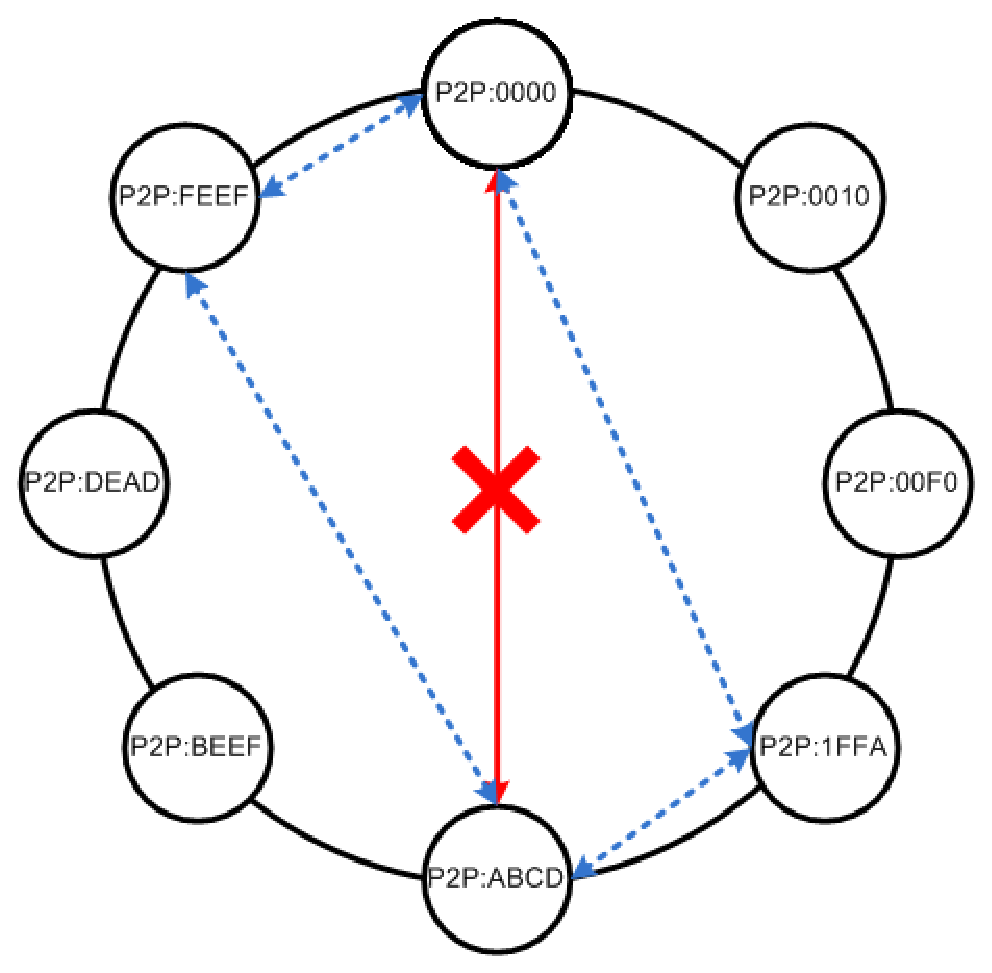
\epsfig{file=figs/relay.png.eps, width=4in}
\caption[Creating relays]{Creating relays across the node address space,
when direct connectivity is not possible.  Two members, 0000 and ABCD,  desire
a direct connection but are unable to directly connect, perhaps due to NATs or
firewalls.  They exchange neighbor information through the overlay and connect
to one of each other's neighbors, creating an overlap.  The overlap then
becomes a relay path (represented by dashed lines), improving performance over
routing across the entire overlay.}
\label{fig:relay}
\end{figure}

Additionally, I have added the feature to exchange arbitrary information along
with the neighbor list.  Thus far, I have implemented systems that pass
information about node stability (measured by the age of a connection) and
proximity (based upon ping latency to neighbors).  Furthermore, when overlap
changes, another mechanism can determine which subset of the peers to use; for
example, a peer may only route through the fastest or more stable overlap in
the set.

To verify the usefulness of two-hop over overlay routing, I performed
experiments and share the results in Section~\ref{relay_motivation}.  In a live
system, I have verified the accuracy and usefulness of the latency-based relay
selection algorithm in Section~\ref{relay_eval}.

\subsection{Motivation for Relays in the Overlay}
\label{relay_motivation}

The purpose of this experiment is to quantify the performance benefits of
autonomic relays.  For this experiment I used the MIT King data
set~\cite{king_data}, which contains all-to-all latencies between 1,740
well-distributed Internet hosts.  Various sizes of networks up to 1,740 nodes
were evaluated 100 times each.  The experiments were executed by running the
Brunet in simulated mode.  Once at steady state, I then calculated the average
all-to-all latency for all messages that would have taken two overlay hops or
more, the average of the low latency relay model, and the average of single hop
communication.  In the low latency relay model, each destination node form a
connection to the source node's physically closest peer as determined via
latency (in a live system by application level ping).  Then this pathway is
used as a two-hop relay between source and node.  I only look at two overlay
hops and more, as a single hop would not necessarily benefit from the work and
would be the cause of a triangular inequality.  

\begin{figure}
\centering
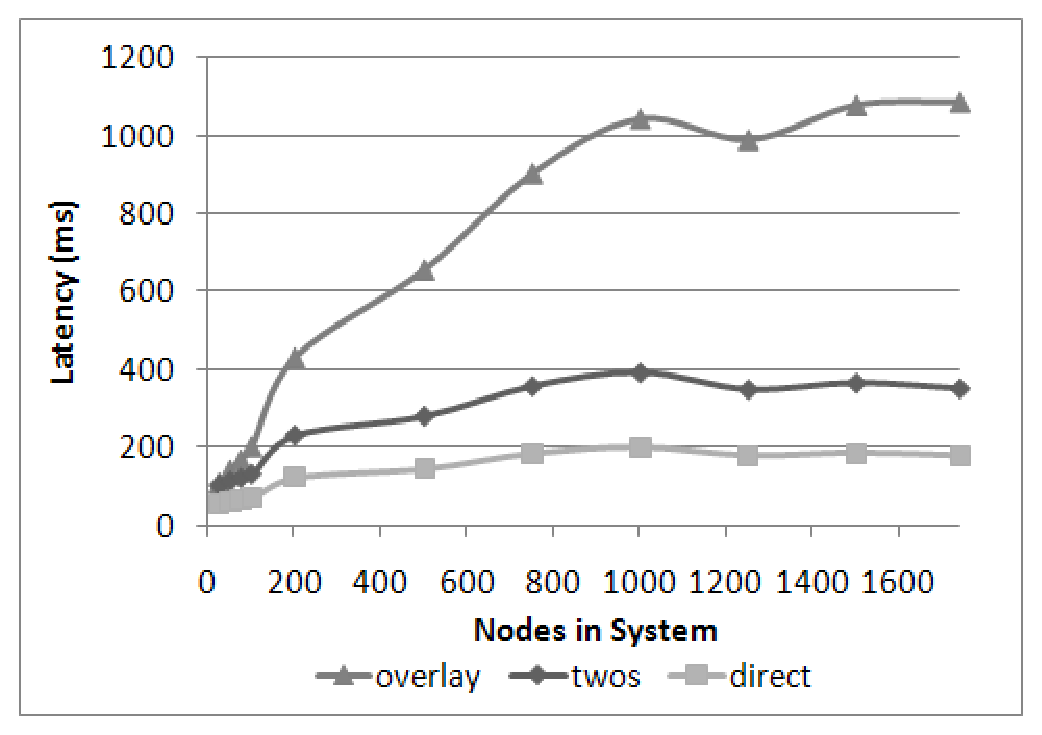
\epsfig{file=figs/relay_motivation.png.eps, width=4in}
\caption[The evaluation of relays]{A comparison of the average all-to-all overlay
routing, two-hop relay, and direct connection latency in a Structured P2P
environment, Brunet, using the King data set.}
\label{fig:simulated_relays}
\end{figure}

The results are presented in Figure~\ref{fig:simulated_relays}.  The initial
starting size for the network was set to 25, because network sizes around 20
and under tend to be fully connected due to the connectivity requirements of
the system.  It is not until the network size expands past 100 and towards 200
nodes that relays become significantly beneficial.  At 100 nodes, there is
approximately a 54\% performance increase, whereas at 200 there is an 87\%
increase and it appears to grow proportionately to the size of the pool.  The
key take away is that latency-bound applications using a reasonably sized
overlay would significantly benefit from the use of two-hop relays.

\subsection{Comparing Relay Selection}
\label{relay_eval}

In this experiment, I share my experiences of testing the use of latency-aware
relays using the public P2P pool running on Planet-Lab as well as Hamachi-Free
and Hamachi-Pro relays.  Due to Hamachi not supporting relays in Linux, this
experiment was performed in Windows Vista 64-bit.  Hamachi is discussed in
greater depth in Chapter~\ref{chap:vpns}.  The testing platform consists of two
virtual machine located on the same host with a firewall preventing them from
establishing direct connections.  All experiments were repeated 5 times using a
clean configuration each time.  In Hamachi, this meant that the server would
need to re-evaluate NAT traversing capabilities and the optimal relay to use.
In Brunet, this meant a new node ID and establishing relays with peers in
different regions of the overlay.  The results are presented in
Table~\ref{tab:relay_eval}.

\begin{table}
\caption[Relay comparison]{Results of the evaluation comparing latency and
bandwidth of Hamachi relays and IPOP latency-aware autonomic relay selection.}

\centering
\begin{tabular*}{\textwidth}{@{\extracolsep{\fill}}
l
S[table-format=2.1,table-number-alignment=right]
S[table-format=2.2,table-number-alignment=right]
S[table-format=4.1,table-number-alignment=right]
S[table-format=4.2,table-number-alignment=right]
@{}
}

\hline &
\multicolumn{2}{c}{Latency} &
\multicolumn{2}{c}{Bandwidth}

\\ \hline &
\multicolumn{1}{c}{(ms)} &
\multicolumn{1}{c}{stdev} &
\multicolumn{1}{c}{Kbit/s} &
\multicolumn{1}{c}{stdev} \\ \hline
Hamachi-Free & 60.8 & 2.54 & 40.2 & 0.87 \\
Hamachi-Pro & 60.2 & 1.68 & 1000 & 1.29 \\ 
Latency-aware & 58.1 & 35.5 & 2245 & 1080 \\ \hline
\end{tabular*}
\label{tab:relay_eval}
\end{table}

As Hamachi was started and figured out that NAT traversal was not possible, it
began using multiple different relays as evident by several different ping
times.  Eventually Hamachi settled on a relay server and it appeared to be the
same one every time, for both Hamachi-Free and Hamachi-Pro.  The only
difference between Hamachi-Pro and Hamachi-Free is that in Pro there is a
bandwidth cap of approximately 1 Mbit/s whereas Free is limited to 40 Kbit/s.

Brunet has nodes both on Planet-Lab but also dedicated systems for
Archer~\cite{archer}.  These machines are at Universities and thus have a high
bandwidth and low latency connection to the testing site.  As witnessed by the
results, it appears that in most if not all these experiments peers had a low
latency connection to a University compute resource and it was chosen ahead of
Planet-Lab.

The two take aways are the benefit of being able to dynamically deploy relay
servers and reuse compute nodes as relay systems.  As the network grows, there
may be need to implement some form of bandwidth limit at relay nodes.

\section{Policies for Establishing Direct Connections}

Routing through a ring-structured overlay using a greedy routing algorithm
takes $log(N)$ time and adds $log(N)$ overall bandwidth for a single message.
Therefore, sending messages frequently between two peers through the overlay is
not cost effective.  What is not apparent through the algorithmic complexity
analysis is the fact that many paths in an overlay can be inefficient due to
peers routing through distant parts of the world or having limited bandwidth.
Less frequently, packets routed via the overlay can just disappear due to nodes
disconnecting or packet drops across the Internet.  To address this, Ganguly et
al.~\cite{wow} made a system for creating adaptive shortcuts.

Adaptive shortcuts enable peers to establish direct links with each other using
Brunet's builtin NAT traversal capabilities.  The approach taken by Ganguly et
al. was to monitor incoming packets from remote peers and after a certain
threshold was passed the system automatically makes a direct connection to the
remote peer.  As a result of this transparency, software using the overlay
could simply start this service without making any additional changes to the
application.  

\subsection{Limitations}

Unfortunately this approach comes with limitations.  There was never any
systematic understanding of behaviors that should signify the creation of a
direct link or when a direct link should be closed.  Thus applying the layer
naively could result in connection churn, which would have ramification on the
routability of the network.  Thus a compromise was made to have it enabled only
for selected traffic, which in the case as described by Ganguly et
al.~\cite{wow} was IP or VN traffic.

Two issues made the approach no longer feasible:  the increase in size of the
overlay network and the securing of IP links.  The Internet drops packets at
approximately .00835\% of the time according to the data provided by
iPlane~\cite{iplane}.  This compounded with the fact that an overlay message
may take $log(N)$ hops significantly increases the likelihood of a packet
dropping before arriving at its destination.  Adding a security model makes
this even more complicated, because a trusted link must be established before
routing any messages between the end points.  In the case of DTLS (datagram
transport layer security), this can result in 6 messages traversing the
overlay~\ref{fig:dtls}, prior to the first IP packet.  If peers must first
establish a trusted link and then transmit a certain amount of packets in a
given time, there is a reasonable chance that they may never naturally trigger
the creation of an adaptive link.

In practice, it was quite common for this not to succeed and, in fact, security
links were often times not even formed.  To verify this, I implemented a
network profiling tool and deployed it on to PlanetLab.  The monitoring tool
measured the delay and success of sending messages between the node and every
other node in the overlay.  The drop rate and latency for a round trip message
per hop distance between two peers are presented in
Figure~\ref{fig:drop_rate_plab} and Figure~\ref{fig:latency_plab},
respectively.  The data in those figures is compared to data retrieved from
iPlane, which makes it clear that PlanetLab exacerbates the situation.  While
this is a well-known issue, it is a very important conclusion since many of the
public systems provided by my research group rely on PlanetLab.

\begin{figure}
\centering
\includegraphics[width=4.5in]{figs/latency_plab.eps}
\caption[Latency in PlanetLab deployment]{Average latency in a round trip
message between two nodes specified by the amount of hops between them.  The
PlanetLab average is compared against data available from iPlane.  The CDF
(cumulative distribution function) for node distance is also plotted for
reference.}
\label{fig:latency_plab}
\end{figure}

\begin{figure}
\centering
\includegraphics[width=4.5in]{figs/drop_rate.eps}
\caption[Drop rate in PlanetLab deployment]{Average drop rate in a round trip
message between two nodes specified by the amount of hops between them.  The
PlanetLab average is compared against data available from iPlane.  The CDF for
node distance is also plotted for reference.}
\label{fig:drop_rate_plab}
\end{figure}

\subsection{On-Demand Connections}

Before defining a new architecture, I measured the network traffic of active
and idle applications that were of interest to typical P2P VPNs,
Condor~\cite{condor0} and data transfers.  Data transfers tend to be simple, if
they are TCP driven, first a TCP link must be established, then data
transferred, and finally the link is closed.  Condor is a job schedule
management tool, which is discussed in more depth in
Chapter~\ref{chap:gridappliance}.  The important aspect for this section is
understanding that all nodes in a Condor pool have a relationship with a
manager node.  Their behavior is to initially send a registration message
containing the details of the node and thereafter to send a one-way message
stating their presence every 5 minutes or so.

The next step was determining the cost of creating a connection versus routing
via the overlay.  This cost needs to consider that before a single IP packet
can be routed, a security link must be established.  In Brunet, the creation of
a link requires 1 round trip message across the overlay, whereas the security
link, as mention earlier, takes 3.  So it is intuitive that sending a single
packet secured through an end-to-end channel via a direct link is far more
efficient than doing so via the overlay.  So instead of having a meter
determining when to create connections, connections should be made as soon as
there is interest in communication, in other words, ``on-demand.''  In a DHT
system, this may be done prior to sending or retrieving data from the DHT.  In
a VPN, this may be during the mapping of IP to P2P as described in
Section~\ref{vpns:arp}, which occurs before secure link establishment.
Unfortunately, this has the side affect of not being transparent to
applications using the P2P software's interface at the cost of being more
responsive.

The creation of on-demand connections results in a higher frequency of
connection establishment.  As a result, better heuristics are necessary in
order to determine when to close unused connections.  Using the profiling
information retrieved before with regards to Condor's one-way ``heartbeat''
messages, it was important that a connection was only closed if it was unused
in both directions.  Otherwise the manager would be constantly closing
connections and peers would randomly disappear from Condor for periods of time.
An algorithm that seems to have worked so far is based upon something I call a
time-based cache.  Initially, entries are stored in a hashtable; after a
certain period of time, they are moved to a second hashtable, and those in the
second hashtable are lost.  If an entry is accessed while in the second
hashtable or not at all, it is added to the first hashtable and if applicable
removed from the second hashtable.  When an entry is removed from the cache, it
causes an eviction notice, which results in the connection being removed.  The
timer is based upon a 7.5 minute timer, so that an inactive connection will be
closed within 7.5 to 15 minutes.

The applicability of on-demand connections compared to Chota was evaluated
using the simulator with 1,024 nodes and a drop rate of 0.00925\% as found on
PlanetLab.  The On-demand connections were established using the exact semantics
of the On-demand protocol; however, the behavior of establishing Chota
connections is a little complicated, since the traffic behavior of successful
and unsuccessful connection attempts is not identical.  To address this, I
simulated an ideal Chota situation:  the nodes optionally establish a security
connection via the overlay, then they exchange a round trip message, and
finally establish a direct connection between each other.  The On-demand
approach involved optionally creating a security connection followed by the
direct connection.  

\begin{figure}
\centering
\includegraphics[width=3.5in]{figs/connections.eps}
\caption[Time to form a direct connection]{CDF for direct connection
establishment of secure and security-free Chota and On-demand connections in an
overlay of 1,024 nodes and a drop rate of 0.835\%.}
\label{fig:connections}
\end{figure}

While this evaluation model creates a highly ideal situation for Chota
etablishment.  The results in Figure~\ref{fig:connections} make it clear that
Chota is not ideal for this type of application and that security only makes
the issues worse.  The On-demand connections show a significant improvement, but
there still exists an obvious issue with connection establishment that will
only be made worse as the system expands.  Perhaps using multiple paths on the
overlay can improve this situation packet drops on the overlay may have high
correlation rather than being uniformly random.

In application, this modification made the Archer, which uses both secure links
and Condor, significantly more stable.  As the system expanded, nodes were
constantly appearing and disappearing, users jobs were being lost due to
disconnectivities, and users were complaining about being unable to even submit
jobs into the system.  Since the change, the issues have been resolved.

\section{Broadcasting IP Broadcast and Multicast Packets Via the Overlay}

The use of a private virtual overlay enables a new method for sending multicast
and broadcast packets. In the original approach to IPOP, broadcasting a packet
to the entire overlay  is not suitable because the overlay could consist of
peers from other VPNs and those not even involved with VPN operations, while
approaches that generate unicast messages when a broadcast or multicast packet
arrives at the VPN (e.g. by querying a DHT key where all peers in the VPN would
place their overlay address so that they could receive the packets) do not
scale well. The abstraction of a private virtual overlay enables scalable
broadcasting within a VPN because the only peers in the private overlay are
peers for a single VPN.  Like the broadcast revocation discussed earlier, IP
broadcasting and multicasting use the method described in
Appendix~\ref{broadcast} to efficiently distribute messages.  Though in VPN
situations, many peers may already have connections to most if not all of their
VPN peers, thus the broadcast algorithm has been modified to allow a peer to
select how many peers they would like to forward the message to.  Otherwise in
many cases, this algorithm will degenerate into one similar to the previous
approach.  

The overlay broadcast method for IP broadcast and multicast can easily be
analytically compared to the original DHT method.  A message routed via the
overlay will take approximately $\log(N)$ hops.  So for the DHT method, this
involves $N$ messages with $\log(N)$ hops each or $N\log(N)$ messages total and
completing in a total time of $\log(N)$ excluding the limitations of bandwidth.
Whereas efficient overlay takes exactly $N$ messages and completes in
$\log^2(N)$ time.  The overlay broadcast significantly reduces bandwidth, which
can have a direct effect on the success of packets actually making it to the
end peer.  Also as the overlay grows in size, storing all peers inside a single
DHT may create other problems that cannot be resolved easily through analytical
modeling.

\section{Full Tunnel VPN Operations}
\label{full_tunnel}

The configuration detailed so far describes a split tunnel: a VPN connection
that handles \emph{internal VPN traffic only, not Internet traffic}.  Prior to
this work, only centralized VPNs currently support full tunnel: providing the
features of a split tunnel in addition to securely forwarding \emph{all their
Internet traffic} through a VPN gateway.  A full tunnel provides network-layer
privacy when a user is in a remote, insecure location such as an open wireless
network at a coffee shop by securely relaying all Internet traffic through a
trusted third party, the VPN gateway.  Both models are illustrated in
Figure~\ref{fig:tunnel}.

\begin{figure}
\centering
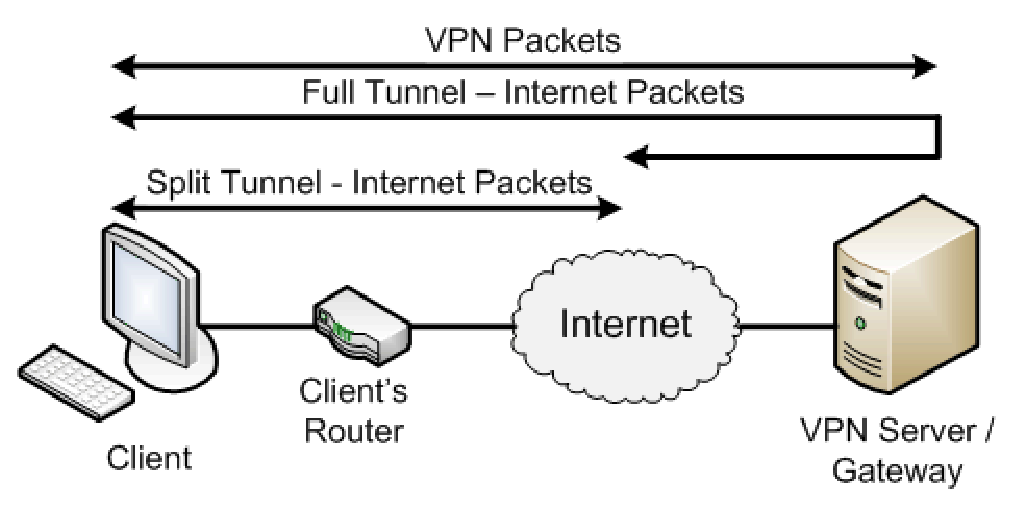
\epsfig{file=figs/tunnel.png.eps, width=4in}
\caption[An example of both full and split tunnel VPN modes]{An example of both
full and split tunnel VPN modes.  In both, packets for the server are sent
directly to the server.  In split tunnel mode, Internet packets bypass the VPN
and are routed directly to the Internet.  In full tunnel mode, Internet packets
are first routed to the VPN gateway, and then to their Internet destination.}
\label{fig:tunnel}
\end{figure}

Central VPN clients use full tunneling through a routing rule swap, setting the
default gateway to be an endpoint in the VPN subnet and traffic for the VPN
server is routed explicitly to the LAN gateway.  This rule swap causes all
Internet packets to be routed to the VN device and the VPN software can then
send them to the remote VPN gateway.  At the VPN gateway, the packet is
decrypted and delivered to the Internet.  A P2P system encounters two
challenges in supporting full tunnels:  P2P traffic must not be routed to the
VPN gateway and there may be more than one VPN gateway.  I address these issues
and provide a solution to this problem in Section~\ref{full_tunnel}.

The challenges faced in a decentralized P2P VPN are providing decentralized
discovery of a VPN gateway and supporting full tunnel mode in a P2P environment
such that all P2P traffic is sent to the intended receiver directly instead of
through the gateway.  The remainder of this section covers gateway and
client solutions to address these challenges.

\subsection{The Gateway}
\label{the_gateway}
A gateway can be configured through NAT software, like masquerading in IPtables
or Internet Connection Sharing with Windows.  This automatically handles the
forwarding of packets received on the NAT interface to another interface
bringing the packet closer to its destination.  Similarly, incoming packets
on the outgoing interface must be parsed in order to determine the destination
NAT client.

Following from the original design of the VPN state machine in
Figure~\ref{fig:vn}, if a VPN is a gateway, the VPN state machine no longer
rejects packets, when the destination is not in the VPN subnet, though when the
VPN gateway mode is disabled these packets are still rejected.  When enabled,
all Internet and non-VPN based traffic is written to the TAP device setting the
destination Ethernet address to the TAP device.  The remaining configuration is
identical to other members of the system as packets from the Internet will
automatically have the clients IP as the destination as a product of the NAT.
To provide for dynamic, self-configuring systems, VPN gateways announce their
availability via an entry in the DHT.  As future work, this approach can be
explored to provide intelligent selection and load balancing of gateways.

\subsection{The Client}
VPN Clients wishing to use full tunnel must redirect their default traffic to
their VN device.  In the prototype VPN model, a virtual IP address is allocated
for the purpose of providing distributed VN services DHCP and DNS.  This same
address is used as the default gateway's IP.  Because this IP address never
appears in a Internet bound packet, only its Ethernet address does, as shown in
Figure~\ref{fig:tunnel_packet}, this approach enables the use of any and
multiple remote gateways.

\begin{figure}
\centering
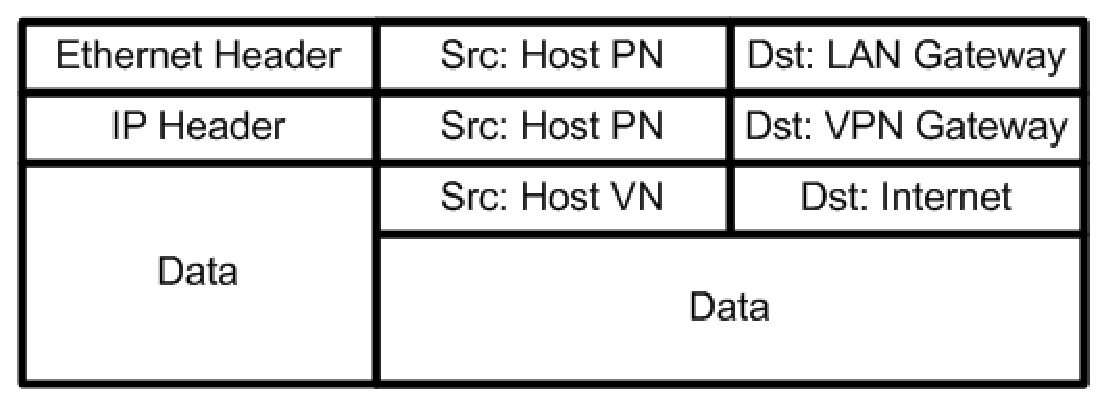
\epsfig{file=figs/tunnel_packet.png.eps, width=4in}
\caption[The contents of a full tunnel Ethernet packet]{The contents of a full
tunnel Ethernet packet.  PN and VN are defined as physical and virtual network,
respectively.}
\label{fig:tunnel_packet}
\end{figure}

To support full tunnel mode, the VPN's state machine has to be slightly modified
to handle outgoing packets destined for IP addresses outside of the VPN, only
rejecting them when full tunnel client mode is disabled.  When enabled, the VPN
software sends packets to the remote peer acting as a full tunnel gateway.
Likewise, incoming packets that have a source address outside the subnet should
not be rejected but instead the overlay address should be a certified VPN
gateway prior to forwarding the packet.

To select a remote gateway, peers query the DHT.  As there may be multiple
gateways in the system, the peer randomly selects one, forwarding packets to
that node.  To ensure reliability, when the client has not heard from the
gateway recently, the client sends a liveness query to the gateway.  If the
gateway is down, the taken pessimistic approach finds a new gateway when
the next Internet packet arrives.

The real challenge in applying full tunnel VPN mode to P2P VPNs is the nature
of the P2P system, namely dynamic connections.  Peers do not know ahead of time
what remote peer connections will be thus a simple rule switch does not work.
The original approach was to watch incoming connection requests and adding
additional routing rules on demand, though this is only reasonably feasible
with UDP as a TCP handshake message would need to be intercepted and potentially
replayed by the local host in order to enable the rule and allow proper routing.
The real drawback of the approach though is that UDP messages can easily be
spoofed by remote peers enabling unsecured Internet packets to be leaked in the
public environment.  Even if the connections are secured, it could take some
time for the peers to recognize a false connection attempt and delete the rule.

A solution to the security problem is to have all traffic directly routed to
the VN device with no additional routing rules.  The VN is then responsible for
filtering P2P traffic and forwarding it to the LAN's gateway via Ethernet
packets.  In the VPN application, outgoing IP packets' source ports are
compared to VPN application's source ports.  Upon a match, the VPN application
directs the packet to the LAN's gateway.  The three steps involved in this
process are translating the source IP address to match the physical Ethernet's
IP address, encapsulating the IP packet in an Ethernet packet with a randomly
source address~\cite{sc09} and the destination the LAN's gateway, and sending
the packet via the physical Ethernet device.  Sending an Ethernet packet is not
trivial as Windows lacks support for this operation and most Unix systems
require administrator privilege.  An alternative, platform independent solution
uses a second TAP device bridged to the physical Ethernet device, allowing
Ethernet packets to be sent indirectly through the Ethernet device via the TAP
device.  Because the solution results in incoming packets to arrive at a
different IP address than the actual original source IP address TCP does not
work in this solution.  This method has been verified to work on both Linux and
Windows using OS dependent TAP devices and bridge utilities.

\subsection{Full Tunnel Overhead}
\label{full_tunnel_eval}

\begin{center}
\begin{table}
\caption[Full tunnel evaluation]{Latency results comparing full tunnel
approaches measured in ms.  Legend: GW Pri - gateway's VPN address, GW Pub -
gateway's VPN address, Ethernet - full tunnel Ethernet packet method, Routing -
full tunnel routing rule switch, None - split tunnel or no VPN.}
\begin{tabular*}{\textwidth}{@{\extracolsep{\fill}}
l
S[table-format=2.1,table-number-alignment=right]
S[table-format=2.1,table-number-alignment=right]
S[table-format=2.1,table-number-alignment=right]
@{}
}

\hline &
\multicolumn{1}{c}{Google} &
\multicolumn{1}{c}{GW Pri} &
\multicolumn{1}{c}{GW Pub} \\ \hline
Ethernet & 70.6 & 12.9 & 13.9 \\ 
Routing & 71.4 & 13.2 & 11.0 \\ 
None & 66.1 & N/A & 10.9 \\ \hline
\end{tabular*}
\label{tab:full_tunnel_eval}
\end{table}
\end{center}

While the full tunnel client method effectively resolves the lingering problem
of ensuring that all packets in a full tunnel will be secure, it raises an
issue:  could the effect of having all packets traverse the VPN application be
prohibitively expensive.  Analysis of this approach compares it with one that
uses the traditional routing rule switch.  Figure~\ref{tab:full_tunnel_eval}
present the ping time from a residential location to one of Google's IP
addresses using a gateway located at the University of Florida when the VPN is
in split tunnel mode, full tunnel using the routing rule switch, and full
tunnel using Ethernet forwarding.  The results express that there is negligible
difference between the full tunnel approaches.  One interesting result is the
latency to gateways public address in the routing test, which most likely is a
result of the ping being sent insecurely avoiding the VPN stack completely.

\chapter{AD-HOC, DECENTRALIZED GRIDS}
\label{chap:gridappliance}

``Give a man a fish, feed him for a day.  Teach a man to fish, feed him for a
lifetime'' -- Lau Tzu

Large-scale grid computing projects such as TeraGrid and Open Science Grid
provide researchers vast amounts of compute resources but with requirements
that could limit access, results delayed due to potentially long job queues,
and environments and policies that might affect a user's work flow. In many
scenarios and in particular with the advent of Infrastructure as a Service
(IaaS) cloud computing, individual users and communities can benefit from less
restrictive, dynamic systems that include a combination of local resources and
on-demand resources provisioned by one or more IaaS provider.  These types of
scenarios benefit from flexibility in deploying resources, remote access, and
environment configuration.

Grid computing presents opportunities to combine distributed resources to form
powerful systems.  Due to the challenges in coordinating resource configuration
and deployment, researchers tend to either become members of existing grids or
deploy their own private resources.  The former approach is limited by lack of
flexibility in the environment and policies, while the latter requires
expertise in systems configuration and management.  Though there exists a
wealth of middleware available, including resource managers such as
Condor~\cite{condor0}, Torque (PBS)~\cite{torque}, and Sun Grid
Engine~\cite{grid_engine}, many see the cost of installing and managing these
systems as being greater than their usefulness and as a result turn to
inefficient ad hoc resource discovery and allocation.  To combine resources
across multiple domains solutions there exist solutions such as the Globus
Toolkit~\cite{globus} or gLite~\cite{glite}; however, these tool sets come with
their own challenges that require the level of expertise most researchers in
fields outside of information technology lack.

With the recent advent of cost-effective on-demand computing through
Infrastructure as a Service ``clouds'', new opportunities for user-deployed
grids have arisen; where, for example, a small local computer cluster can be
complemented by dynamically provisioned resources that run ``cloud-burst''
workloads.  However, while cloud-provisioned resources solve the problem of
on-demand instantiation, the problem of how to {\em configure} these resources
to seamlessly and securely integrate with one's infrastructure remains a
challenge.  In particular, considering that users may provision resources from
multiple IaaS providers, the configuration demands are similar to a distributed
grid: while a cloud image can be encapsulated with a grid computing stack, it
still needs configuration in terms of allocating and distributing the
appropriate certificates, network configuration to establish end-to-end
connectivity, and proper configuration of the middleware to establish worker,
submit, and scheduler nodes.  

In this chapter, I present techniques that reduce the entry barrier in terms of
necessary expertise and time investment in deploying and extending ad hoc,
distributed grids.  To verify this assertion, I have implemented a system
supporting these ideas in the ``Grid Appliance,'' which as will be
demonstrated, allows users to focus on making use of a grid while minimizing
their efforts in setting up and managing the underlying components.  The core
challenges solved by my approach include:

\begin{itemize}
\item decentralized directory service for organizing grids,
\item decentralized job submission,
\item grid single sign on through web services and interfaces,
\item sandboxing with network support,
\item and all-to-all connectivity despite network asymmetries.
\end{itemize}

\begin{figure}
\centering
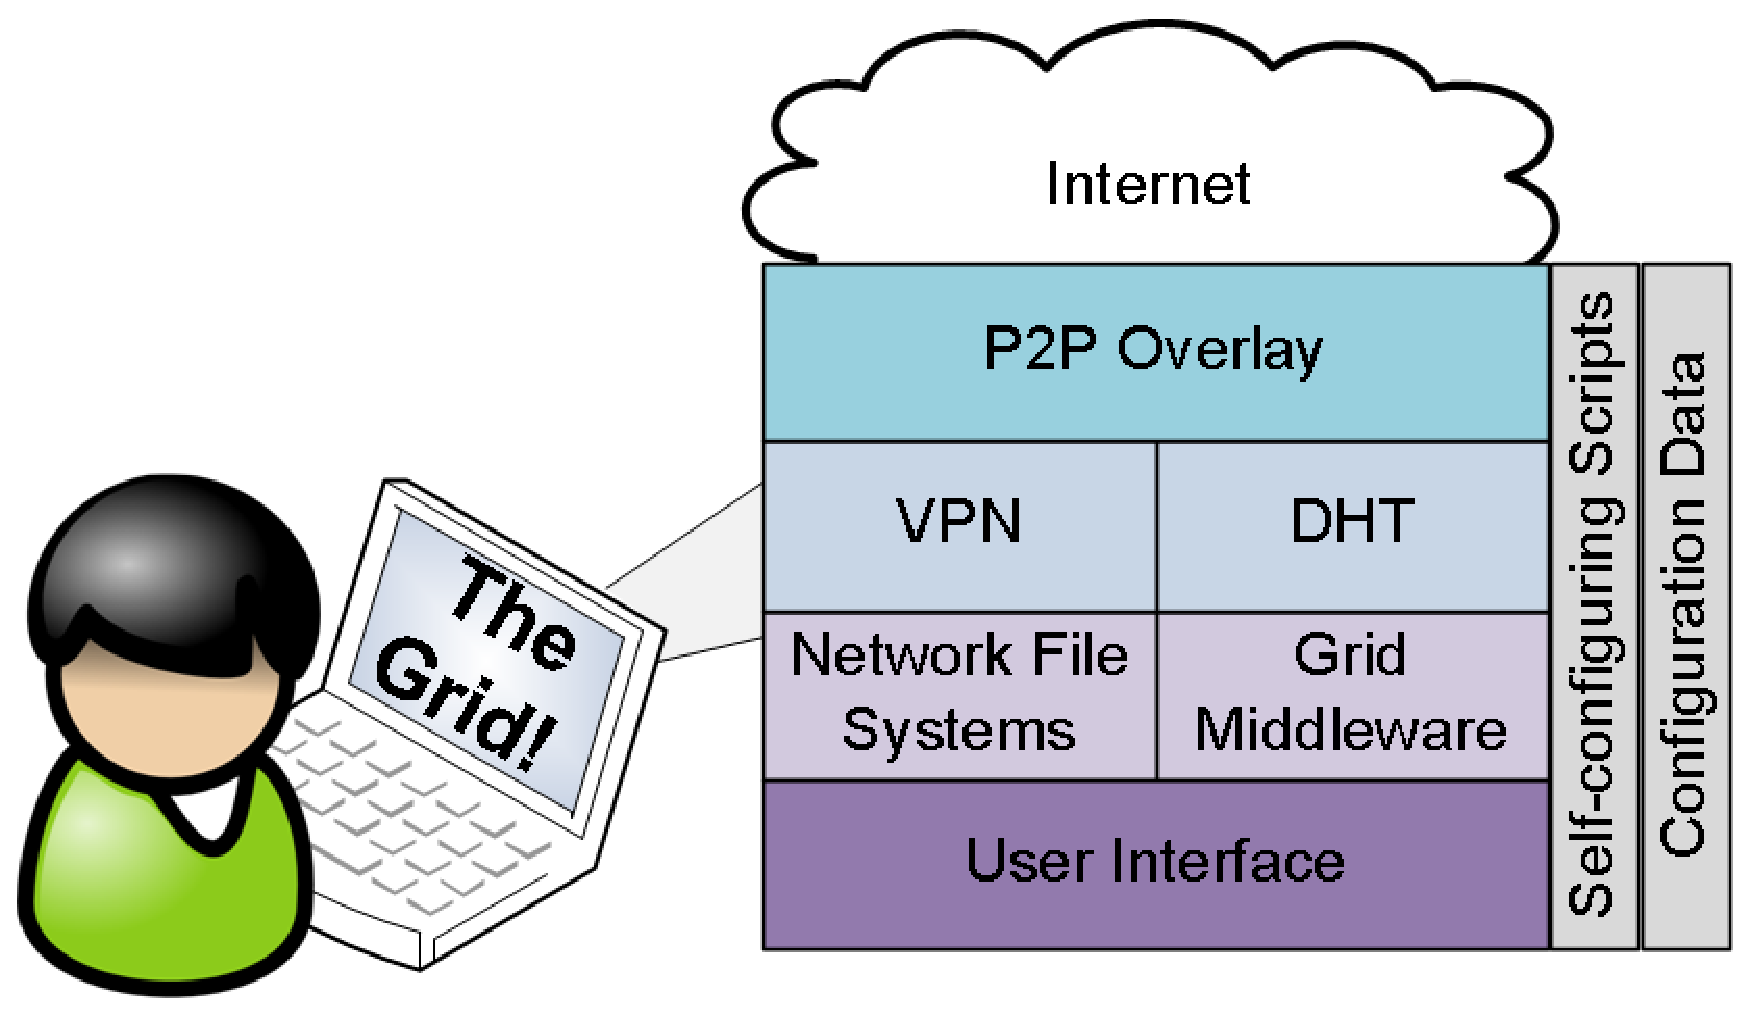
\includegraphics[width=4in]{figs/appliance_overlays.eps}
\caption[Grid Appliance middlware]{The ``Grid Appliance'' connects to other
resources over a common network.  Both the grid middleware and the VPN use the
P2P overlay to configure and connect the user to other members of the grid.
The process uses configuration data provided by the web interface to
self-configure the system using information available in the P2P network.}
\label{fig:appliance}
\end{figure}

The ``Grid Appliance'' project and concepts have been actively developed and
used in several projects for the past six years.  Of these projects, Archer, a
distributed grid for computer architecture research,
has demonstrated the feasibility and utility of this approach by
deploying a shared collaborative infrastructure spanning clusters across six US
universities, where the majority of the nodes are constrained by network
address translation (NAT).  Every resource in Archer is configured in the same,
simple manner:  by deploying a ``Grid Appliance'' that self-configures to join a
wide-area grid.  Researchers interested or desiring the ability to access both
grid resources and specialized commercial simulation tools (such as Simics) can
easily use and contribute resources from this shared pool with little effort
by joining a website, downloading a configuration image and a virtual
machine (VM), and starting the VM inside a VM manager (VMM).  Upon completion of
the booting process, users are connected to the grid and able to submit and
receive jobs.

At the heart of my approach lies a P2P (peer-to-peer) infrastructure based upon
a distributed hash table (DHT) useful for decentralized configuration and
organization of systems.  Peers are able to store key, value pairs into the DHT
and to query the DHT with a key and potentially receive multiple values
efficiently.  The DHT provides discovery and coordination primitives for the
configuration of a decentralized P2P virtual private network (VPN), which
supports unmodified applications across a network overlay.  The DHT is also
used for the decentralized coordination of the grid.  Users can configure their
grid through a web interface, which outputs configuration files that can be
used with the ``Grid Appliance.''

The techniques described in this paper have many applications.  The basic
system supports the creation of local grids by starting a virtual machine on
the computers intended for use within the grid and using LAN multicast for
discovery.  It allows users to seamlessly combine their dedicated grids with
external resources such as workstations and cloud resources.  The level of
familiarity with security, operating systems, and networking is minimal as all
the configuration details are handled as components of the system.  Management
of the system including users and network configuration utilizes a social
networking like group interface, while deployment uses pre-built virtual
machine images.  A graphical overview of the system is illustrated in
Figure~\ref{fig:appliance}.

These techniques simplify the tethering of resources across disparate networks
The setup of security, connectivity, and their continuous management imposes
considerable administrative overhead, in particular when networks are
constrained by firewalls and NAT devices that prevent direct communication with
each other, and which are typically outside the control of a user or lab.  Our
approach integrates decentralized systems behind NATs in a manner that does not
require the setup of exceptions and configuration at NAT/firewall by system
administrators.

The rest of the paper is as follows.  Section~\ref{wow} highlights of my
research groups previous work to provide background for my contributions in
this paper.  In Section~\ref{architecture}, I describe the components of the
``Grid Appliance'' WOW.  Section~\ref{case_study} provides a case study of a
grid deployment using standard grid deployment techniques compared to our
``Grid Appliance,'' describing qualitatively the benefits and evaluating
quantitatively the overheads of this approach.  I share my experiences from
this long running project in Section~\ref{lessons_learned}.  Finally,
Section~\ref{related_work} compares and contrasts other solutions to these
problems.

\section{WOWs}
\label{wow}

This work furthers the vision began by myself and my research lab in earlier
described as work wide-area overlay of virtual workstations~\cite{wow} (WOW).
The WOW paper established the use of virtualization technologies, primarily
virtual networking and virtual machines, to support dynamic allocation of
additional resources in grids that span wide area networks.  For reference, the
extensions made in this paper to the WOW concept are means for the dynamic
creation of grids with support for security, decentralized access, and
user-friendly approaches to grid management.  This section covers the
development of WOWs over the years as it relates to other publications and as
means to distinguish the contributions made by me and in this chapter.

\subsection{P2P Overlays}

Peer-to-peer or P2P systems create environments where members have a common
functionality.  P2P systems are often used for discovery in addition to some
user-specific service, such as voice and video with Skype or data sharing with
BitTorrent.  Many forms of P2P have autonomic features such as self-healing and
self-optimization with the ability to support decentralized environments.  As I
will show, this makes their application in the system very attractive.

For the ``Grid Appliance,'' I have chosen to use Brunet~\cite{brunet}, a type of
structured overlay.  Structured overlays tend to be used to construct
distributed hash tables (DHT) and in comparison to unstructured overlays
provide faster guaranteed search times ($O(\log N)$ compared to $O(N)$, where N
is the size of the network).  The two most successful structured overlays are
Kademlia~\cite{kademlia}, commonly used for decentralized BitTorrent, and
Dynamo~\cite{dynamo}, to support Amazon's web site and services.

Brunet support for NAT traversal makes it unique from other structured
overlays.  Originally in the WOWs~\cite{wow}, Brunet facilitated the dynamic
connections amongst peers in the grid.  Since then, it has been extended to
support DHT with atomic operations~\cite{pcgrid07}, efficient relays when
direct NAT traversal fails~\cite{groupvpn}, resilient overlay structure and
routing~\cite{hpdc08_0}, and cryptographically secure
messaging~\cite{groupvpn}.

\subsection{Virtual Private Networks}

A common question with regards to this work is ``why VPNs?''  The core reason
is connectivity.  IPv4 (Internet Protocol version 4) has a limited address
space, which has been extended through the use of NAT allowing a single IP to
be multiplexed by multiple devices.  This creates a problem; however, as it
breaks symmetry in the Internet limiting the ability for certain peers to
become connected and which peers can initiate connections.  With the advent of
IPv6 (Internet Protocol version 6), the situation might improve, but there are
no guarantees that NATs will disappear nor can users be certain that firewalls
will not be in place that inhibit symmetry.  A VPN circumvents these issues, so
long as the user can connect to the VPN, as all traffic is routed through a
successfully connected pathway.

The problem with traditional VPN approaches is management overhead including
maintaining resources on public IP addresses and establishing links amongst
members in the VPN.  The VPN used in the system is called IPOP~\cite{groupvpn,
ipop}.  IPOP (IP over P2P), as the name implies, uses a P2P overlay (Brunet) to
route IP messages.  By using P2P, maintaining dedicated bootstrap nodes have
less overhead, my approach with IPOP allows an existing Brunet infrastructure
to bootstrap independent Brunet infrastructures in order to isolate IPOP
networks in their own environments~\cite{bootstrapping}.

Once IPOP has entered its unique Brunet overlay, it obtains an IP address.  IP
address reservation and discovery relies on Brunet's DHT.  Each VPN stores its
P2P identifier into the DHT at the generated by the desired IP address, such
that the key, value pair is $(hash(IP), P2P)$.  In order to ensure there are no
conflicts, the storing of this value into the DHT uses an atomic operation,
which succeeds only if no other peer has stored a value int $hash(IP)$.

The process for creating connections begins when IPOP receives an outgoing
message.  First it parses the destination address and queries the DHT for the
remote peers P2P address.  The peer then attempts to form a secure, direct
connection with the remote peer using Brunet's secure messaging layer.  Once
that has formed, packets to that IP address are directed over that secure link.

In my original design~\cite{vtdc}, the virtual network was secured through a
kernel-level IPsec stack, a model kept through the first generation Archer
deployment.  This approach only secures virtual network links between parties
and does not secure the P2P layer; furthermore, in IPsec configuration each
peer requires a unique rule for every other peer, which limited the maximum
number of peers in the VPN.  Securing the P2P layer is important, otherwise
malicious users could easily derail the entire system, but securing with IPsec
would practically negate the benefits of the P2P system, because of network
configuration issues related to NATs and firewalls.  In modern deployments, I
have employed the security layer at the P2P layer, which in turn also secures
virtual networking links.

For grids that rely upon VPNs to connect resources and users, this can impose
the need for a certificate for the VPN and one for the grid.  Though in our
approach, I avoid this problem by using a VPN that allows a user to verify the
identity of a remote peer and obtain its certificate, and have taken advantage
of hooks in grid software that are called to verify a remote peers
authenticity.  In other words, user access is limited by the VPN and identity
inside the grid is maintained by that same certificate.  This might not be
possible if all users were submitting from the same resources but is feasible
in the system since each user submits from their own system.

\subsection{Virtual Machines in Grid Computing}

Earlier work~\cite{fig_grid} advocated the use of virtual machines (VMs) in
grid computing for improved security and customization.  Others
since~\cite{sandbox, dve, ourgrid_paper} have been established VMs as means for
sandboxing, that is environments that allow untrusted users to use trusted
resources in a limited fashion.  VMs run as a process on a system, where
processes running inside the VM have no access to the host operating system.
Furthermore, VMs can have limited or no networking access as controlled by the
host, which effectively seals them in a cage or sandbox protecting the hosts
environment.  VMs are also useful for customization and legacy applications,
since a developer can configure the VM and then distribute it as an appliance,
with the only requirement on the end user being that they have a VM software or
manager.  Quantitatively, previous work has shown that CPU-bound tasks perform
fairly well running with no more than 10\% overhead and in some cases 0\%,
which is the case with VMs like Xen.

While not a direct correlation to grid computing, clouds have benefited
significantly from VMs.  VMs are the magic behind cloud infrastructures that
provide IaaS, such as EC2.  In these environments, users are able to create
customized instances, or packaged operating systems and applications, inside of
cloud environments, share with each other, and dynamically create or shutdown
them as necessary.  While the application of clouds is generic, it can easily
be applied towards grids.  A user can create push excess jobs into the cloud,
when there is overflow, high demands, or the user does not want to maintain
their own hardware.  One challenge, however, is the dynamic creation of a grid
as well as extension of an existing grid using the cloud, challenges that are
addressed in this paper.

\section{Architectural Overview}
\label{architecture}

My approach attempts to reuse as many available components to design a grid
middleware generic enough that th ideas can be applied to other middleware
stacks.  As a result, my contribution in this chapter and in particular this
section focuses primarily on the following key tasks:  making grid construction
easy, supporting decentralized user access, sandboxing the users environment,
limiting access to the grid to authorized identities, and ensuring priority on
users own resources.  

\begin{center}
\begin{table}
\caption{Grid middleware comparison.}
\footnotesize{
\begin{tabular}[c]{p{1.6cm}p{3.25cm}p{3.4cm}p{3.2cm}p{3.05cm}} \hline
& Description & Scalability & Job queue / submission site & API Requirements \\ \hline
Boinc &
Volunteer computing, applications ship with Boinc and poll head node for data
sets &
Not explicitly mentioned, limited by the ability of the scheduler to handle
the demands of the client &
Each application has a different site, no separation from job queue and
submission site &
Boinc API and middleware bundling required
\\
BonjourGrid &
Desktop grid, use zeroconf / Bonjour to find available resources in a LAN &
No bounds tested, limits include multicasting overheads and processing power
of job queue node &
Each user has their own job queue / submission site &
None \\
Condor &
High throughput computing / on demand / desktop / etc / general grid computing &
Over 10,000$^{1}$ &
Global job queue, no limit on submission sites, submission site communicates directly with worker nodes &
Optional API to support job migration and check pointing \\
PastryGrid &
Use structured overlay Pastry to form decentralized grids &
Decentralized, single node limited by its processing power, though
collectively limited by the Pastry DHT &
Each connected peer maintains its own job queue and submission site &
None \\
PBS / Torque~\cite{torque} &
Traditional approach to dedicated grid computing &
up to 20,000 CPUs$^{2}$ &
Global job queue and submission site &
None
\\
SGE &
Traditional approach to dedicated grid computing &
Tested up to 63,000 cores on almost 4,000 hosts$^{3}$ &
Global job queue and submission site &
None
\\
XtremWeb &
Desktop grid, similar to Condor but uses pull instead of push, like Boinc &
Not explicitly mentioned, limited by the ability of the scheduler to handle
the demands of clients &
Global job queue, separate submission site, optionally one per user &
No built-in support for shared file systems
\\ \hline
\end{tabular}
}
\label{tab:grid}
\end{table}
\end{center}

\addtocounter{footnote}{1}
\footnotetext[\value{footnote}]{\url{http://www.cs.wisc.edu/condor/CondorWeek2009/condor\_presentations/sfiligoi-Condor\_WAN\_scalability.pdf}}
\addtocounter{footnote}{1}
\footnotetext[\value{footnote}]{\url{http://www.clusterresources.com/docs/211}}
\addtocounter{footnote}{1}
\footnotetext[\value{footnote}]{\url{http://www.sun.com/offers/docs/Extreme\_Scalability\_SGE.pdf}}

\subsection{Web Interface and the Community}

Before deploying any software or configuring any hardware, a grid needs
organization including certificate management, grid access, user account
management, and delegation of responsibilities.  These are complex questions,
which can be challenging to address, though for less restrictive systems, like
a collection of academic labs sharing clusters, they may be very easy.  One of
the professors could handle the initial authorization of all the other labs and
then delegate to them the responsibility of allowing their affiliates, such as
students and scholars access.

For academic environments, grids become more challenging when the professor or
worse yet students must maintain the certificates, handling certificate
requests, and placing signed certificates in the correct location.  Our
solution to this potentially confusing area was a group interface, akin to
something like Facebook's or Google's groups.  Albeit, those types of groups
are not hierarchal, which is a necessity in order to have delegated
responsibilities.  Thus I have a two layer approach, a grid group for members
of the grid trusted by the grid organizers and user groups for those who are
trusted by those in the grid group.  Members of the grid group can create their
own user groups.  A member of a user group can gain access to the grid by
downloading grid configuration data available within the user group web
interface.  This configuration data comes in the format of a disk image, when
added to a ``Grid Appliance'' VM, it is used to obtain the user's credentials
and enabling them to connect to the grid.

To give an example, consider the computer architecture grid, Archer.  Archer
was seeded initially by the University of Florida, so my group and I are the
founders and maintainers of the Archer grid group.  As new universities and
independent researchers have joined Archer, they request access to this group.
Upon receiving approval, they then need to form their own user group so that
they can allow others to connect to the grid.  So a trusted member might create
a user group titled ``Archer for University X'' and all members of university X
will apply for membership in that group.  The creator can make decisions to
either accept or deny these users.  Once the user has access, they will
download their configuration data formatted as a virtual disk image and the
``Grid Appliance'' VM and start the ``VM.''  After starting the VM, the user
will be connected to the grid and able to submit and receive jobs.

\begin{figure}
\centering
\epsfig{file=figs/system.eps, width=\textwidth}
\caption[Grid Appliance deployment scenario]{An example deployment scenario:
obtaining configuration files, starting the appliance, and connecting with a
resource manager.}
\label{fig:system}
\end{figure}

Joining is easy; a grid requires a user to sign onto a website and download a
configuration data, which can then be used on multiple systems.  To support
this process, the configuration data contains cryptographic information that
facilitates acquisition of a signed certificate from the web interface through
XML-RPC over HTTPS (Extensible Markup Language Remote Procedure Call over
Hypertext Transfer Protocol Secure).  The process begins by either booting the
``Grid Appliance'' or restarting a ``Grid Appliance'' service.  When starting
the service will detect if there is new configuration data, and if there is, it
contacts the web interface with the cryptographic information and a public key.
The web interface verifies the user's identity, retrieves their profile from
its database and binds that information with the public key to create a
certificate request, which will then be signed and returned to the user.

With a public web interface, I have been able to create a variety communities.
One of particular interest is not the grid itself but rather a bootstrapping
community for grids.  The web interface has been designed to support many grid
groups, so too has the P2P infrastructure as it supports bootstrapping into
unique private overlays for individual grids by means of Brunet's ability to
support recursive bootstrapping.  By using the public interface, users have an
opportunity to reuse a public bootstrap infrastructure and only need to focus
on the configuration of their VPN and grid services, which has been trivialized
to accepting or denying users access to a group and turning on resources.  We
would like to note that there is no need to make an explicit public grid
community through the web interface, since all ``Grid Appliances'' come with a
default configuration file that will connect them to an insecure public grid.  

\subsection{The Organization of the Grid}

The previous section focused facilitation of grid configuration using the web
interface and skirted the issues of detailed configuration and organization.
The configuration of the grid mirrors that of the connection process.  The
first tier group maps to a common grid and each grid maps to a VPN.  Thus when
a user creates a new grid group, they are actually configuring a new VPN, which
involves address range, security parameters, user agreements, and the name of
the group.  The system provides defaults for address range and security
parameters, so users can focus on high level details like the user agreement
and the grid's name.

As mentioned earlier, the second tier of groups enables members in the grid
group to provide access to their community.  It is also the location that users
download their configuration data.  The configuration files come in three
flavors: submission, worker, or manager.  Worker nodes strictly run jobs.
Submission nodes can run jobs as well as submit jobs into the grid.  Manager
nodes are akin to head nodes, those that manage the interaction between worker
and submission nodes.

While the configuration details are handled by the web interface and scripts
inside the ``Grid Appliance,'' organization of the grid, more specifically the
linking of worker and submission nodes to manager nodes, relies on the DHT.
Managers store their IP addresses into the DHT at the key \emph{managers}.
When workers and clients join the grid, they automatically query this key,
using the results to configure their grid software.  Managers can also query
this key to learn of other managers to coordinate with each other.

\subsubsection{Selecting a Middleware}

My grid composition is largely based upon a desire to support a decentralized
environment, while still retaining reliability and limiting documentation
support efforts.  As there exist many middlewares to support job submission and
scheduling, I surveyed available and established middleware to determine how
well they matched my requirements.  My results are presented in
Table~\ref{tab:grid}, which covers most of the well established middleware and
some recent research projects focused on decentralized organization.

Of the resource management middlewares surveyed, I chose to use Condor as it
matches closest with my goals due to its decentralized properties and focus on
desktop grids.  Condor allows multiple submission points, a non-trivial
obstacle in some of the other systems.  Additionally, adding and removing
resources in Condor can be done without any configuration from the managers.
Conversely, in SGE and Torque, after resources have been added into the system,
the administrator must manually configure the manager to control them.  Most
scheduling software assumes that resources are dedicated, while Condor supports
opportunistic cycles, by detecting the presence of other entities and will
suspend, migrate, or terminate a job, thus enabling desktop grids.  A common
drawback to established middlewares is the requirement of a manager node;
having no manager in an ad hoc grid would be ideal.

\subsubsection{Self-Organizing Condor}

While the requirement of a central manager may be undesirable, they can easily
be run inside a VM and Condor supports the ability to run many in parallel
through the use of ``flocking~\cite{flocking}.'' Flocking allows submission
sites to connect to multiple managers.  This serves two purposes: 1) to provide
transparent reliability by supporting multiple managers and 2) users can share
their resources through their own manager.  Flocking allows each site to run
its own manager or share the common manager.  

To configure Condor, manager IP addresses are stored into the DHT using the key
\emph{managers}.  Joining peers query the DHT to obtain a list of managers,
selecting one randomly to use as its primary manager with the result used for
flocking.  If the system prefers managers from its group, it will randomly
contact each manager in an attempt to find a match, selecting one at random if
no match is found.  Until a manager is found, the process repeats every 60
seconds.  Upon finding a manager, the state of the system is verified every 10
minutes and new managers are added to the flock list.

\subsubsection{Putting It All Together}

The following summarizes the configuration and organization of the grid.
Minimally a grid will constitute a manager, some workers, and a submitter.
Referencing Figure~\ref{fig:system} step ``1,'' during system boot, without
user interaction, each machine contacts the group website to obtain a valid VPN
certificate.  Whereupon, it connects to the P2P overlay whose bootstrap peers
are listed inside the configuration file, ``step 2.''  At which point, the
machine starts the VPN service running on top of the P2P overlay, also part of
step ``2.'' The self-configuring VPN creates a transparent layer hiding from
the user and administrators the complexity in setting up a common fabric that
can handle potential network dynamics.  Machines automatically obtain a unique
IP address and find their place inside the grid.  For a manager machine, this
means registering in the DHT (not shown), while clients and workers search for
available managers by querying the DHT, step ``3;'' IPOP translates the IP to a
P2P address, step ``4;'' and then client contacts the manager directly, step
``5.''

\subsection{Sandboxing Resources}

As tasks can run on worker and potentially submission nodes, I have devised
means to sandbox the environments that do not limit user interactions with the
system.  While more traditional approaches to sandboxing emphasize a separation
between worker and submission machine, in actual deployments, very few users
explicitly deploy worker machines, most are submission machines.  Thus I
developed sandboxing techniques to limit the ability of submitted jobs on
systems that are simultaneously being used for submission.  So these sandboxing
technique considers more than just locking down the machine but also ensuring a
reasonable level of access.

\subsubsection{Securing the Resources}

The core of my sandboxing approach is to limit attacks to software in the
system and not poorly configured user space, such as poorly chosen passwords or
resources external to the ``Grid Appliance.''  All jobs are run as a set of
predefined user identities.  When the jobs are finished executing, whether
forcibly shutdown or completed successfully, all processes from that user are
shutdown, preventing malicious trojan attacks.  Those users only have access to
the working directory for the job and those with permission for everybody.
Escalation of privilege attacks due to poor passwords are prevented by
disallowing use of ``su'' or ``sudo'' for these users.  Finally, network access
is limited to the VPN, thus they are unable to perform denial of service
attacks on the Internet.

Additionally, systems can be configured such that the only network presented to
them is that of the virtual network.  To support this, IPOP has been enhanced to
support a router mode, which can be bridged to a virtual machine adapter
running on the host machine that connects to the network device running inside
the VM.  Not only does this improve performance, due to reduced I/O overhead,
the same virtual network router can be used for multiple VMs.

To ensure that submit machines still have a high level of functionality without
risking the system to external attacks even from users on the same network,
user services are run only on a ``host-only'' network device within the virtual
machine.  This includes an SSH server and a Samba or Windows File Share.  The
user name matches that from the website, while the password defaults to
``password.''  I would like to note that file sharing services work the
opposite to that of host to guest as most VMs already have in place.  Instead
users can access their files on the VM from the host.  This was done to limit
potential attacks on submission machine.

\subsubsection{Respecting the Host}

Another aspect of sandboxing is respecting the usage of the host.  While Condor
can detect host usage on a machine it is running, when run inside a VM it
cannot detect usage on the host.  Thus it is imperative to support such a
configuration otherwise my approach would be limited in that it can only be
run during idle times.  In the ``Grid Appliance'', this is addressed by running
a light-weight agent on the host that communicates to the VM through the second
Ethernet interface.  The agent discovers a VM through multicast service
discovery executed only on "host-only" virtual network devices.  When a user
accesses the host, the agent notifies a service in the VM, which results in
running tasks being suspended, migrated, or terminated.  The machine remains
off limits until there has been no user activity for 10 minutes.

\subsubsection{Decentralized Submission of Jobs}

From the administrator's perspective, not requiring a submission machine is
also a form of sandboxing.  Maintaining a worker machine requires very low
overhead, since jobs and their associated files are removed upon the completion
of a job and corrupted workers can be deleted and redeployed.  Maintaining a
submission machine means user accounts, network access, providing data storage,
and trusting users to play nicely on a shared resource.  So having users be
able to submit from their own resources reduces the overhead in managing a
grid.  It does come with a consequence, most grids provide shared file systems,
which are statically mounted in all nodes.  In a dynamic grid that might have
multiple shares, this type of approach may not be very feasible.

All is not lost, for example, Condor provides data distribution mechanisms for
submitted jobs.  This can be an inconvenience, however, if only a portion of
the file is necessary, as the entire file must be distributed to each worker.
This can be particularly true with disk images used by computer architecture
simulations and applications built with many modules or documentation.  To
support sparse data transfers and simplify access to local data, each ``Grid
Appliance'' has a local NFS share exported with read-only permission.  To
address the issue of mounting a file system, there exists a tool to
automatically mount file systems, autofs. autofs tool works by intercepting
file system calls inside a specific directory, parsing the path, and mounting a
remote file system.  In the ``Grid Appliance,'' accessing the path
\url{/mnt/ganfs/hostname}, where hostname is either the IP address or hostname
of an appliance, will automatically that appliance's NFS export without the
need for super-user intervention.  Mounts are automatically unmounted after a
sufficient period of time without any access to the mounted file system.  

\section{Deploying a Campus Grid}
\label{case_study}

I now present a case study exploring a qualitative and quantitative comparison
in deploying a campus grid and extending it into the ``Cloud'' using
traditional techniques versus a grid constructed by ``Grid Appliance.''  One of
the target environments for the ``Grid Appliance'' is resources provided in
distributed computer labs and many small distributed clusters on one or more
university campus as shown in Figure~\ref{fig:unconnected}.  The goals in both
these cases are to use commodity software, where available, and to provide a
solution that is both simple but creates an adequate grid.  In both cases,
Condor is chosen as the middleware, which is a push scheduler and by default
requires that all resources be on a common network thus a VPN will be utilized.
Additionally, in this section, I cover details of the ``Grid Appliance'' that
did not fit in the context of previous discussions in the paper.

\subsection{Background}

In this case study, I will compare and contrast the construction of two types
of grids:  a static grid configured by hand and a dynamic grid configured by
the ``Grid Appliance.''  Each grid is initially constructed using resources at
the University of Florida and later extended to Amazon's EC2 and Future Grid at
India University using Eucalyptus.  Each environment has a NAT limiting
symmetric communication: University of Florida resources are behind two layers,
first an ``iptables'' NAT and then a Cisco NAT; EC2 resources have a simple 1:1
NAT; and the Eucalyptus resources appear to have an ``iptables'' NAT.

\begin{figure}
\centering
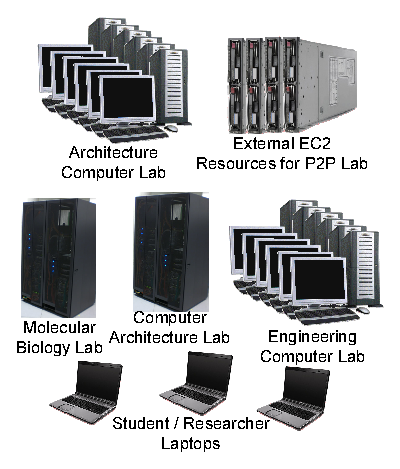
\epsfig{file=figs/unconnected.eps, width=3.25in}
\caption{A collection of various computing resources at a typical university.}
\label{fig:unconnected}
\end{figure}

\subsection{Traditional Configuration of a Campus Grid}

A VPN must be used to connect the resources due to the lack of network symmetry
across the sites.  There exists a wealth of VPNs available~\cite{hamachi,
openvpn, tinc} and some explicitly for grids~\cite{violin, vine, vnet}.  For
simplicity sake, OpenVPN was chosen due to the simplicity in its configuration.
In reality, OpenVPN makes a poor choice because it is centralized, thus all
traffic between submitter and worker must traverse the VPNs server.  Whereas
others in the list are distributed and thus allow nodes to communicate
directly, but in order to do so, manual setup is required, a process, that
would overwhelm many novice grid deployers.  In all these cases, the VPN
requires that at least a single node have a public address, thus I had to make
a single concession in the design of this grid, that is, the OpenVPN server
runs on a public node.

In order to connect to OpenVPN, it must know the server's address and have a
signed certificate.  While typically, most administrators would want a unique
private key for each machine joining the grid, in my case study and
evaluation, I avoided this process and used a common key, certificate pair.  In
doing so, there are potential dangers, for example, if any of the machines were
hijacked, the certificate would have to be revoked and all machines would be
rendered inoperable.  To create a properly secured environment, each resource
would have to generate or be provided a private key, a certificate request
submitted to the certificate authority, and a signed certificate provided to
the resource.

With the networking and security components in place, the next step is
configuring grid middleware.  Prior to deploying any resources, the manager
must be allocated and its IP address provider to other resources in the system.
Submission points are not a focus on this case study, though in general most
systems of this nature have a single shared submission site.  The challenges in
supporting multiple submission points in this environment include creating
certificates same as worker nodes,  requiring users to configure OpenVPN and
Condor, and handling NFS mounts.  Whereas having a single submission point
creates more work for the system administrator as mentioned earlier.  Both
approaches have their associated costs and neither is trivial.  The evaluation
assumes a single user submitting from a single resource.

To address potential heterogeneity issues.  An administrator would need to
collaborate with others to ensure that all resources are running a common set
of tools and libraries.  Otherwise an application that works well on one
platform could cause a segmentation fault on another, through no fault of the
user, but rather due to library incompatibilities. 

To export this system into various clouds, an administrator starts by running
an instance that contains their desired Linux distribution and then installing
the grid utilities like Condor and OpenVPN.  Supporting individualization of
the resources is challenging.  The simplest approach is to store all the
configuration in that instance including the single private key, certificate
pair as well as the IP address of the manager node.  Alternatively, the
administrator could build an infrastructure that receives certificate requests
and returns a certificate.  The IP address of the manager node and of the
certificate request handler could be provided to the cloud via user data, a
feature common to most IaaS clouds that allows users to provide either text or
binary data that is available via a private URL inside a cloud instance.

\subsection{Grid Appliance in a Campus Grid}

All these configuration issues are exactly the reasons why ``Grid Appliance''
and its associated group Web interface are desirable for small and medium scale
grids.  The first component is deciding which web interface to use, public
(\url{www.grid-appliance.org}) or private hosted on their own resources.
Similarly, users can deploy their own P2P overlay or use the shared overlay.

The web interface enforces unique names for both the users and the groups.
Once the user has membership in the second tier of groups, they can download a
file that will be used to automatically configure their resources.  As
mentioned earlier, this handled obtaining a unique signed certificate,
connecting to the VPN, and discovering the manager in the grid.  Configuration
of the VPN and grid are handled seamlessly, the VPN automatically establishes
direct links with peers on demand and peers configure based upon information
available in the P2P overlay dynamically allowing for configuration changes.

Heterogeneity is a problem that will always exist if individuals are given
governance of their own resources.  Rather than fight that process, the ``Grid
Appliance'' approach is to provide a reference system and then include that
version and additional programs in the resource description exported by Condor.
Thus a user looking for a specific application, library, or computer
architecture can specify that in their job description.  Additionally, by means
of the transparent NFS mounts, users can easily compile their own applications
and libraries and export them to remote worker nodes.

Extending the ``Grid Appliance'' system into the clouds is easy.  The
similarity between a VM appliance and a cloud instance are striking.  The only
difference from the perspective of the ``Grid Appliance'' system is where to
check for configuration data.  Once a user has created a ``Grid Appliance'' in
a cloud, everyone else can reuse it and just supply their configuration data as
the user data during the instantiation of the instances.  As I describe in
Section~\ref{packaging}, creating ``Grid Appliance'' from scratch is a trivial
procedure.

As described in detail earlier, an administrator needs to install the necessary
software either by deploying VMMs and VM appliances or installing ``Grid
Appliance'' packages on Debian / Ubuntu systems.  Additionally, these systems
need to be packaged with the configuration files or floppy disk images.  At
which point, the systems will automatically configure and connect to the grid.
An administrator can verify this by monitoring Condor.  Additional resources
can be added seamlessly, likewise resources can be removed by shutting them off
without direct interaction with the ``Grid Appliance'' or manager node.

\subsection{Comparing the User Experience}

In the case of a traditional grid, most users will contact the administrator
and make a request for an account.  Upon receiving confirmation, the user will
have the ability to SSH into a submission site.  Their connectivity to the
system is instantaneous, their jobs will begin executing as soon as it is their
turn in the queue.  User's will most likely have access to a global NFS.  From
the user's perspective, the traditional approach is very easy and
straightforward.

With the ``Grid Appliance,'' a user will obtain an account at the web
interface, download a VM and a configuration file, and start the VM.  Upon
booting, the user will be able to submit and receive jobs.  To access the grid,
users can either SSH into the machine or use the consoles in the VM.  While
there is no single, global NFS, each user has their own unique NFS and must
make their job submission files contain their unique path.  For the most part,
the user's perspective of the ``Grid Appliance'' approach has much of the same
feel as the traditional approach.  Although users have additional features such
as accessing their files via Samba and having a portable environment for doing
their software development.

\subsection{Quantifying the Experience}

The evaluation of these environments focuses on the time taken to dynamically
allocate the resources, connect to the grid, and submit a simple job to all
resources in the grid.  In both systems, a single manager and submission node
were instantiated in separate VMs.  In the traditional setup, OpenVPN is run
from the manager node.  Each component in the evaluation was run three times.
Between iterations, the submission node and the manager node were restarted to
clear any state.

The times measured include the time from when the last grid resource was
started to the time it reported to the manager node, Figure~\ref{fig:connect},
as well as the time required for the submit node to queue and run a 5 minute
job on all the connected workers, Figure~\ref{fig:run}.  The purpose of the
second test is to measure the time it takes for a submission site to queue a
task to all workers, connect to the workers, submit the job, and to receive the
results; thus a stress test on the VPN's ability to dynamically create links
and verifying all-to-all connectivity.  The tests were run on 50 resources
(virtual machines / cloud instances) in each environment and then on a grid
consisting of all 150 resources with 50 at each site.

\begin{figure}
\centering
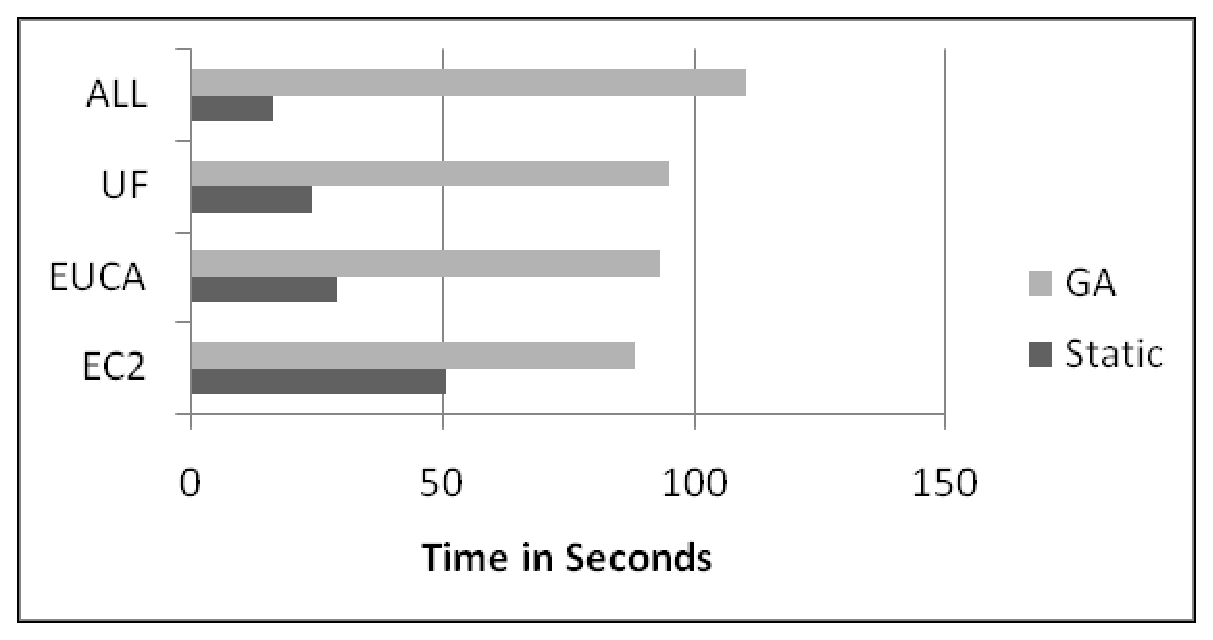
\epsfig{file=figs/connect.eps, width=4in}
\caption[Time to construct a grid]{Comparison of times to construct a grid in
various environments using both a statically configured grid and a grid
constructed by the ``Grid Appliance.''  Legend:  EC2 - Amazon's EC2, Euca -
Indiana University's Eucalyptus, UF - University of Florida's ACIS Lab
resources, Static - OpenVPN, GA - Grid Appliance.}
\label{fig:connect}
\end{figure}

\begin{figure}
\centering
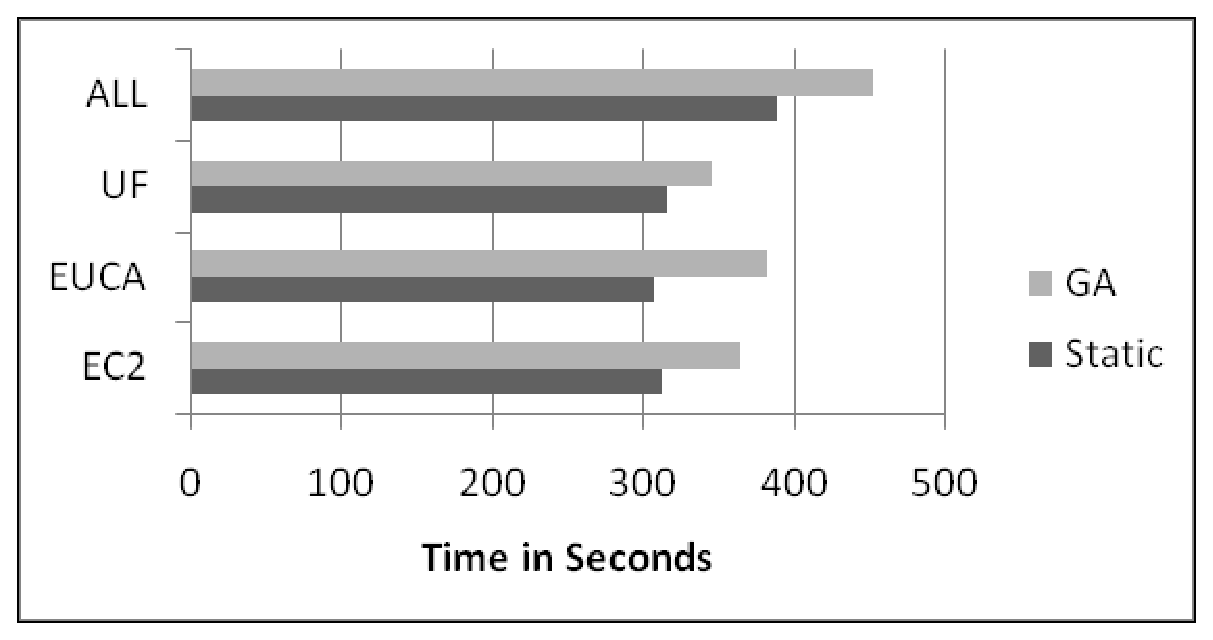
\epsfig{file=figs/run.eps, width=4in}
\caption[Time to run a job on a grid]{Comparison of times to run a 300 second
job on each resource in various grids configured statically and through the
``Grid Appliance.'' Legend:  EC2 - Amazon's EC2, Euca - Indiana University's
Eucalyptus, UF - University of Florida's ACIS Lab resources, Static - OpenVPN,
GA - Grid Appliance.}
\label{fig:run}
\end{figure}

In the previous section, I qualified why the approach was easier than
configuring a grid by hand, though by doing so I introduce overheads related to
configuration and organization.  The evaluation verifies that these overheads
do not conflict with the utility of my approach.  Not only do resources within
a cluster install the VMs and connect to the grid quickly, the clouds do as
well.  While the results were similar, it should be noted that the time
required to configure the static approach was not taken into effect.  A process
that is difficult to measure and is largely reliant on the ability of the
administrator and the tools used.  Whereas the time for the ``Grid Appliance''
does include many of these components.

It should be stated that the evaluation only has a single submission node.  In
a system with multiple submitters, the OpenVPN server could easily become a
bandwidth bottleneck in the system as all data must pass through it, which can
be avoided using IPOP.  Additionally, the current ``Grid Appliance'' relies on
polling with long delays, so as to not have negative effects on the system.
Either shrinking those times or moving to an event based system should
significantly improve the speed at which connectivity occurs.  

\section{Lessons Learned}
\label{lessons_learned}

This section highlights some the interesting developments and experiences, we
have had that do not fit the topics discussed so far.  

\subsection{Deployments}

A significant component of my experience stems from the computational grid
provided by Archer~\cite{archer}, an active grid deployed for computer
architecture research, which has been online for over 3 years.  Archer
currently spans six seed universities contributing over 600 CPUs as well as
contributions and activities from external users.  The Archer grid has been
accessed by hundreds of students and researchers from over a dozen institutions
submitting jobs totaling over 500,000 hours of job execution in the past two
years alone.

The Grid Appliance has also been utilized by groups at the Universities of
Florida, Clemson, Arkansas, and Northwestern Switzerland as a tool for teaching
grid computing.  Meanwhile the universities of Clemson and Purdue are using the
Grid Appliance's VPN (GroupVPN / IPOP) to create their own grid systems.  Over
time, there have been many private, small-scale systems using the shared system
available at \url{www.grid-appliance.org} with other groups constructing their
own independent systems.  Feedback from users through surveys have shown that
non-expert users are able to connect to the public Grid appliance pool in a
matter of minutes by simply downloading and booting a plug-and-play VM image
that is portable across VMware, VirtualBox, and KVM.

\subsection{Towards Unvirtualized Environments}
\label{packaging}

Because of the demands put on Archer in terms of avoiding the overheads of
virtualization and the perceived simplicity of managing physical resources as
opposed to virtual resources running on top of a physical resources, many users
have requested the ability to run Grid Appliances directly on their machine.
Unlike clouds with machine images such as AMIs (Amazon Machine Image) or VM
appliances, physical machines images cannot be easily exported.  Most physical
OS installed on physical machines will need some some custom tailoring to
handle environment specific issues.

With this in mind, I moved away from stackable file systems and towards
creating repositories with installable packages, such as DEB or RPM.  The
implications of packages mean that users can easily produce ``Grid Appliances''
from installed systems or during system installation.  With the VPN router
mode, mentioned earlier, resources in a LAN can communicate directly with each
other rather than through the VPN.  That means if they are on a gigabit
network, they can full network speeds as opposed to being limited to 20\% of
that due to the VPN, overheads discussed in~\cite{sc09}.

\subsection{Advantages and Challenges of the Cloud}

I have had the experience of deploying the ``Grid Appliance'' on three
different cloud stacks:  Amazon's EC2~\cite{ec2}, Future Grid's
Eucalyptus~\cite{eucalyptus}, and Future Grid's Nimbus~\cite{nimbus}.  All of
the systems, encountered so far, allow for data to be uploaded with each cloud
instance started.  The instance can then download the data from a static URL
only accessible from within the instance, for example, EC2 user data is
accessible at \url{http://169.254.169.254/latest/user-data}. A ``Grid
Appliance'' cloud instances can be configured via user-data, which is the same
configuration data used as the virtual and physical machines, albeit zip
compressed.  The ``Grid Appliance'' seeks the configuration data by first
checking for a physical floppy disk, then in specific directory
(\url{/opt/grid\_appliance/var/floppy.img}), followed by the EC2 / Eucalyptus
URL, and finally the Nimbus URL.  Upon finding a floppy and mounting it, the
system continues on with configuration.  Clouds have been also very useful for
debugging.  Though Amazon is not free, with Future Grid, grid researchers now
have free access to both Eucalyptus and Nimbus clouds.  Many bugs can be
difficult to reproduce in small system tests or booting one system at a time.
By starting many instances simultaneously, I have been able to quickly
reproduce problems and isolate them, leading to timely resolutions, and
verification of those fixes.

Beyond the use of extending into clouds for on-demand resources, they are also
very convenient for debugging.  Doing so on Amazon though is not free.
Fortunately, grid researchers now can have free access to Future Grid with both
Eucalyptus and Nimbus style clouds.  I did have to do some tinkering to get
these systems to work.  First, because the user data is binary data and the
communication exchange uses RPC, which may have difficulty handling binary
data, it must be converted to base64 before transferring and converted back
into binary data afterward.  EC2 handles this transparently, if using
command-line tools.  Unfortunately, Eucalyptus and Nimbus do not, even though
Eucalyptus is supposed to be compatible with EC2.

Furthermore, when starting an EC2 instance, networking is immediately
available, whereas with Eucalyptus and Nimbus, networking often times takes
more than 10 seconds after starting to be available. Thus a startup script must
be prepared for networking not to be ready and hence unable to immediately
download user data.  The best approach to deal with this in a distribution
independent manner is to wait until the primary Ethernet interface (eth0) has
an IP and then continuing.

\subsection{Stacked File Systems}

Configuring systems can be difficult, which makes it important to have the
ability to share the resulting system with others.  The approach of actually
creating packages can be overly complicated for novices.  To address this
concern, the original ``Grid Appliance'' supported a built-in mechanism to
create packages through a stackable file system using
copy-on-write~\cite{vtdc}.  In this environment, the VM used 3 disks: the
``Grid Appliance'' base image, the software stack configured by us; a module;
and a home disk.  In normal usage, both the base and module images are treated
as read-only file systems with all user changes to the system being recorded by
the home image, as depicted in Figure~\ref{fig:stackfs}.

\begin{figure}
\centering
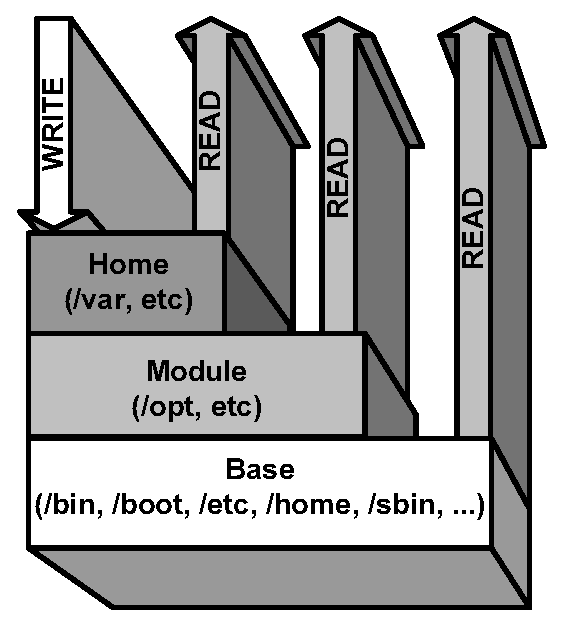
\epsfig{file=figs/stackfs.eps, width=2.5in}
\caption[Grid Appliance stackable file system]{Example of a stackable file
system from the previous ``Grid Appliance.''  A file will be read from the top
most file system in the stack and all writes are directed to Home.}
\label{fig:stackfs}
\end{figure}

To upgrade the system, users replaced their current base image with a newer
one, while keeping their module and home disks.  While the purpose of the
module was to allow users to extend the configuration of the ``Grid
Appliance.''  To configure a module the system would be booted into developer
mode, an option during the boot phase, where only the base and module images
are included in the stacked file system.  Upon completing the changes, a user
would run a script that would clean the system and prepare it for sharing.  A
user could then share the resulting module image with others.

Issues with this approach made it unattractive to continue using.  First, there
exists no kernel level support for stackable file systems, I had to add
UnionFS~\cite{unionfs} to the kernel, adding the weight of maintaining a kernel
unto my shoulders.  While FUSE (filesystem in userspace) solutions exist, they
require modifications to the initial ram disk, which is reproduced
automatically during the installation of every new kernel, furthermore, our
experience with them suggests they are not well suited for production systems.
Additionally, the approach was not portable to clouds or physical resources.
So while I have deprecated the feature for now, I see it as a potential means
to easily develop packages like DEB and RPM.

\subsection{Priority in Owned Resources}

In Archer, seed universities should have priority on the resources at their
university.  Similarly, users should have priority on their contributions.
Otherwise, users will remove their resources from the grid, when they want
guaranteed access.  To support user and group based priorities, Condor has
mechanisms that can be enforced at the server that allow for arbitrary means to
specify user priority for a specific resource.  So the configuration specifies
that if the resource's user or group matches that of the submitter, the
priority is higher than otherwise.  This alone is not sufficient as malicious
users could easily tweak their user name or group to obtain priority on all
resources.  Thus whenever this check is made the user's identity in the
submission information is verified against their P2P VPN certificate.  Failed
matches are not scheduled and are stored in a log at the manager for the
administrator to deal with later.

To support this behavior, the following statements have been added to the
respective system's Condor configuration file:

\begin{tabbing}
Th\=e \=format for this configuration is as follows:\\
\> Job queue (server):\\
\> \> NEGOTIATOR\_PRE\_JOB\_RANK = 10 * (MY.RANK) \\
\> Worker:\\
\> \> GROUP\_RANK = TARGET.Group =?= MY.Group \\
\> \> USER\_RANK = TARGET.User =?= My.User \\
\> \> RANK = GROUP\_RANK $\vert\vert$ USER\_RANK \\
\>  Worker and Submitter:\\
\> \> Group = "Group's Name"\\
\> \> User = "User's Name"
\end{tabbing}

\subsection{Timing in Virtual Machines}

Certain applications, particularly license servers, are sensitive to time.
Because of the nature of grids, there exist possibilities of having
uncoordinated timing, such as improperly specifying the time zone or not using
a network time protocol (NTP) server With regards to VMs,
VMWare~\cite{vmware_timing} suggests synchronizing with the host's time and to
avoid using services like NTP, which may have adverse affects on timing inside
the virtual machine.  While NTP might have some strange behavior, relying on
host time may produce erratic jumps in time that some software cannot handle.
My experiences recommends the use of NTP to address these concerns, which has
resolved many issues with strange software behavior and frustration from users
when their jobs fail due to being unable to obtain a license due to a timing
mismatch.

\subsection{Selecting a VPN IP Address Range}

One challenge in deploying a VPN is ensuring that the address space does not
overlap with that over the environments where it will be used.  If there is
overlap, users will be unable to connect to the VPN.  Doing so will confuse the
network stack, as there will be two network interfaces connected to the same
address space but different networks.  A guaranteed, though not necessarily
practical solution is to run the resource on a VM NAT or a cluster NAT that
does not overlap the IP address space of the VPN.

Users of the ``Grid Appliance'' should not have to concern themselves with this
issues.  Prior work on the topic by Ala Rezmerita et al.~\cite{pvc} recommends
using the experimental address class E ranging between 240.0.0.0 -
255.255.255.254, unfortunately this requires Linux kernel modifications.  With
the amount of bugs and security fixes regularly pushed into the kernel,
maintaining a forked kernel requires a significant amount of time, duplicating
the work already being performed by the OS distribution maintainers.  This
would also limit the ability to easily deploy resources in physical and cloud
environments.  Additionally, users that wanted to multipurpose a physical
resource may not want to run a modified kernel, while in most cloud setups the
kernel choice is limited.

I have since moved towards using the 5.0.0.0 - 5.255.255.255 address range.
Like the class E address space it is unallocated, but it requires no changes to
any operating systems.  The only limitation is that some other VPNs also use
it, thus a user would not be able to run two VPNs on the same address space
concurrently.  This approach is much better than providing kernels or dealing
with network address overlaps.  Interestingly, even with this in place, we
still see some ``GroupVPNs''  using address ranges in normal private network
address ranges for the VPN, like 10.0.0.0 - 10.255.255.255 and 192.168.0.0 -
192.168.255.255.

\subsection{Administrator Backdoor}

While most administrators will agree that most problems that users encounter
are self-inflicted, there are times, when the system is at fault.  Debugging
systems faults in a decentralized system can be very tricky, since it is very
difficult to track down a resource in order to gain direct physical access.
Additionally, having a user bring their resource to an administrator may be
prohibitively complicated, as the user would need to relocate their ``Grid
Appliance'' instance and have network connectivity in order to connect to the
grid and show the problem to the administrator.  To address this and other
concerns that only appear after running the system for long periods of time, we
have supplied an administrator backdoor into all resources by installing our
public ssh key, though users are informed of this and are free to remove it for
privacy concerns.  In typical configurations, this approach might not be
feasible, but because the ``Grid Appliance'' ships with a decentralized VPN
supporting all-to-all connectivity, any resource connected to the VPN is
accessible for remote debugging by an administrator.  Most users involved are
extremely delighted with the process as it has an appearance that the system
``just works.''

\section{Related Work}
\label{related_work}

Existing work that falls under the general area of desktop grids/opportunistic
computing include Boinc~\cite{boinc}, BonjourGrid~\cite{bonjourgrid}, and
PVC~\cite{pvc}.  Boinc, used by many ``@home'' solutions, focuses on adding
execute nodes easy; however, job submission and management rely on
centralization and all tasks must use the Boinc APIs.  BonjourGrid removes the
need for centralization through the use of multicast resource discovery; the
need for which limits its applicability to local area networks.  PVC enables
distributed, wide-area systems with decentralized job submission and execution
through the use of VPNs, but relies on centralized VPN and resource management.

Each approach addresses a unique challenge in grid computing, but none
addresses the challenge presented as a whole: easily constructing distributed,
cross-domain grids.  Challenges that I consider in the design of my system
include allowing submission sites to exist any where without being confined to
complex configuration or highly available, centralized locations; the ability
to dynamically add and remove resources by starting and stopping a a resource;
and the sharing of common servers so that no group in the grid is dependent on
another.  I emphasize these points, while still retaining the ease of use of
Boinc, the connectivity of PVC, and the flexibility of BonjourGrid.  The end
result is a system similar to OurGrid~\cite{ourgrid}; however, OurGrid requires
manual configuration of the grid and networking amongst sites, administration
of users within a site, and limits network connectivity amongst resources,
whereas ``Grid Appliance'' transparently handles these issues with a P2P
overlay and VPN to handle network constraints and support network sandboxing
and a web interface to configure and manage the grid.

With regards to clouds, there exists contextualization~\cite{context}.  Users
construct an XML configuration file that describes how a cloud instance should
be configured and provide this to a broker.  During booting of a cloud
instance, it will contact a third-party contextualization broker to receive
this file and configure the system.  This approach has been leveraged to create
dynamic grids inside the Nimbus cloud~\cite{alien_grid}.  While this approach
can reproduce similar features of the ``Grid Appliance,'' such as creating
grids inside the cloud, there are challenges in addressing cloud bursting,
automated signing of certificates, and collaboration amongst disparate groups.

\chapter{SOCIAL PROFILE OVERLAYS}
\label{chap:spo}

Online social networking has become pervasive in daily life, though as social
networks grow so does the wealth of personal information that they store.  Once
information has been released on a social network, known as a user's profile,
the user and the data are at the mercy of the terms dictated by the social
network infrastructure, which today is typically third-party, centrally owned.
If the social network engages in activities disagreeable to the user, due to
change of terms or opt-out programs not well understood by users such as recent
issues with Facebook's Beacon program~\cite{facebook_beacon}, the options
presented to the user are limited.  The options include leaving the social
network, surrendering their identity and features provided by the social
network; accepting the disagreeable activities; or to petition and hope that
the social network changes its behavior. 

As the use of social networking expands to become the primary way in which
users communicate and express their identity amongst their peers, the users
become more dependent on the policies of social network infrastructure owners.
Recent work~\cite{p2p_socialnetwork} explores the coupling between social
networks and P2P systems as a means to return ownership to the users, noting
that a social network made up of social links is inherently a P2P system with
the aside that they are currently developed on top of centralized systems.
This chapter extends this idea with focus on the topic of topology; that is,
how to organize social profiles that leverage the benefits offered by a
structured P2P overlay abstraction.

Structured P2P overlays provide a scalable, resilient, autonomic platform for
distributed applications.  Structured overlays enable users to easily create
their own decentralized systems for the purpose of data sharing, interactive
activities, and other networking-enabled activities.  This chapter is based
upon my previous work~\cite{groupvpn, bootstrapping} discussed in chapters
\ref{chap:bootstrapping} and \ref{chap:security} to enable social network
profile overlays.  These works address the challenges of bootstrapping secure,
private overlays in environments constrained by network address translators
(NATs) and firewalls through a public overlay used for discovery and as a relay
or communication transport.  

A typical social network consists of users and groups.  Each user has a
profile, a set of friends, and the ability to send and receive private
messages; each group consists of one or more managers, users, and a messaging
board.  Profiles contain user's personal information, status updates, and
public conversations, similar to a message board.  Friends are individuals
trusted sufficiently by a user to view the user's profile.  Private messaging
sends messages discretely between users without leaking the message to other
members.  Groups have similar features, though identity is shared by many
users.

Using this social networking model, I have designed OverSoc.  OverSoc uses a
public overlay as a directory for finding and befriending peers or finding and
accessing groups.  Once group and profile access has been offered, the public
overlay can be used to bootstrap connectivity to existing profile and group
overlays.  Security for a profile is provided by a public key infrastructure
(PKI), where profile owners or group managers are the certificate authorities
(CA) and all members have signed certificates.  The overlay stores profile data
or group information in its distributed data store, supporting decentralized
access using scalable mechanisms regardless of the profile owner's online
presence.  In this chapter, I present the architecture of these overlays, as
presented in Figure~\ref{fig:spo.system}.

\begin{figure}
\centering
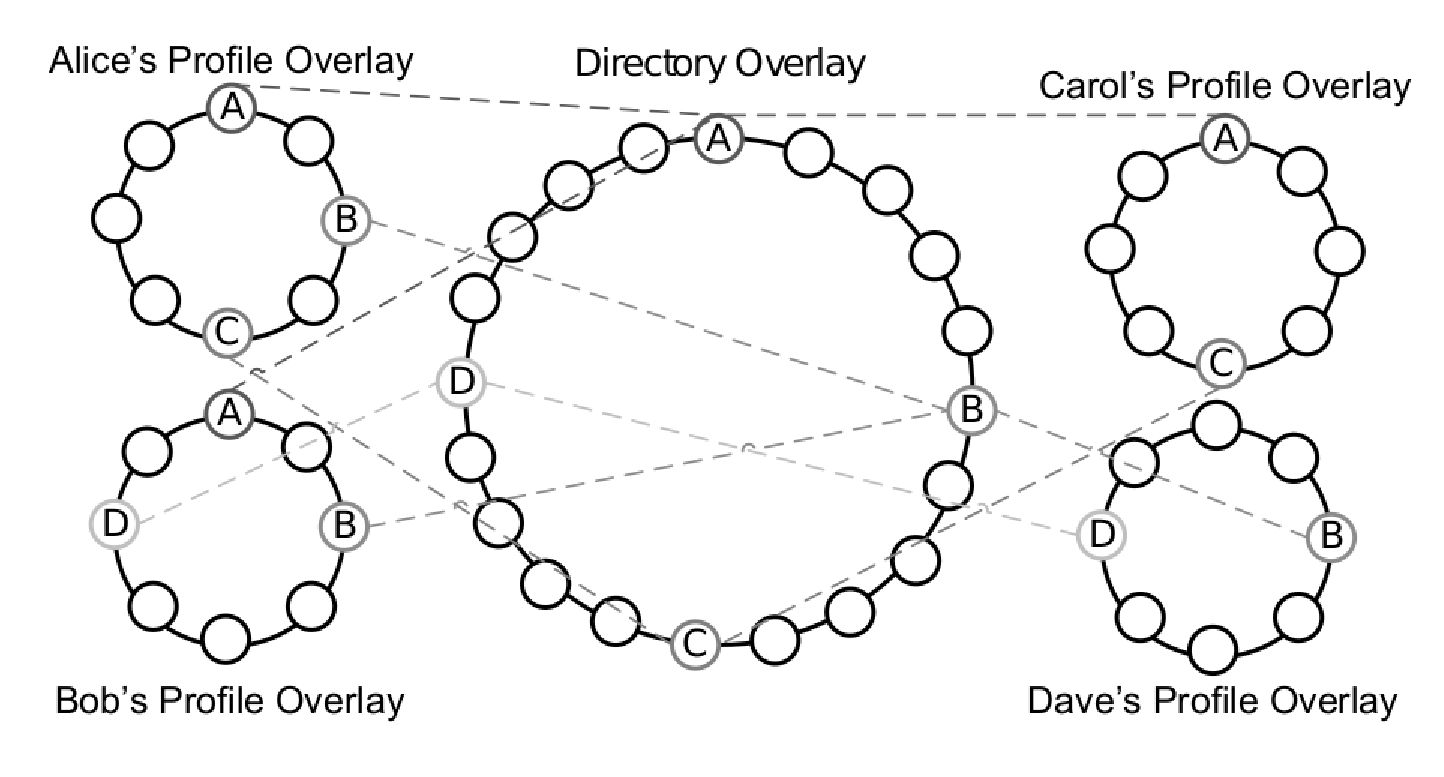
\epsfig{file=figs/subrings.eps, width=\textwidth}
\caption[An example OverSoc social overlay network]{An example OverSoc social
overlay network.  Alice has a friendship with Bob and Carol, hence both are
members of her profile overlay. Bob has a friendship with Alice and Dave but
not Carol; hence Alice and Dave are members of his profile overlay, while Carol
is not.  Each peer has many overlay memberships but a single root represented
by dashed lines in various shades of gray.  For clarity, overlay shortcut
connections are not shown.}
\label{fig:spo.system}
\end{figure}

The rest of this chapter is organized as follows.  Section~\ref{vpo:background}
discusses related work.  Section~\ref{vpo:social_overlays} describes OverSoc,
explaining how to map social networks onto structured P2P overlays.
Section~\ref{vpo:user_interaction} expresses expectations for user interaction in
the system.  In Section~\ref{vpo:outstanding}, I explore some of the remaining
challenges introduced by this approach.  

\section{Related Works}
\label{vpo:background}

In~\cite{peerson}, Buchegger et al. describe how to use a DHT to store social
networking profile.  The DHT provides look-up services for storing meta-data
pertaining to a peer's profile.  Peers query the DHT for updated content from
their friends by hashing their unique identifiers (e.g. friends' email
addresses).  The retrieved meta-data contains information for obtaining the
profile data such as IP address and file version. Their work relies on a PKI
system that provides identification, encryption, and access control.  In
contrast, OverSoc maps individual user profiles and groups to a private overlay
secured by point-to-point encryption and authentication amongst all peers in
the overlay.  The private overlay provides a clean abstraction of access
control, whereby once admitted to a private overlay, users can access a
distributed data store which holds the contents of the owner's profile.

Shakimov et al. in \cite{vis-a-vis} take a different approach by depending on
virtual individual servers (VIS) hosted on a cloud infrastructure such as
Amazon EC2. Friends contact each other's VIS directly for updates.  A DHT is
used as a directory for groups and interest-based searches. Their approach
assumes bidirectional end-to-end connectivity between each VIS, where a profile
is only available during the up time of the VIS.  Because of the demands on
network connectivity and up time, the approach assumes a cloud-hosted VIS and
has difficulty being used on user-owned resources.  OverSoc allows peers to
have  asymmetric connectivity and does not require constant up time through the
use of NAT traversal support and the ability to store the profile in the
overlay's distributed data store.

The approach presented by Cutillo et al. in~\cite{matryoshka} relies on a
central system to host identities and certificates that can then be used to
query a DHT to discover an initial hop in a route to a specific peer through
their circle of friends.  The circle of friends consists of an unstructured
overlay, where direct friends maintain direct connections with the peer, and
outer circles consist of friends of friends and friends of friends of friends.
The main goal of this work is to remove the private components of a profile
from a central entity, whereas OverSoc makes a clean break from all
centralization and enables scalability through distributed replication
techniques.

Unlike the above approaches, the P2P social network presented by Abbas et al.
in~\cite{tribler-osn} uses an unstructured overlay without a DHT where peers
connect directly to each other rather than through the overlay establishing
unique identifiers to deal with dynamic IPs.  Peers cache each other's data to
improve availability, while helper nodes are used to assist with communication
between peers behind NATs.  The approach lacks security and access control
considerations and lacks the guarantees and the simplicity of the abstraction
offered by a structured overlay.

\begin{figure}
\centering
\epsfig{file=figs/friendship_request.eps, width=\textwidth}
\caption{Alice requests and receives a friendship from Bob.}
\label{fig:friend_request}
\end{figure}

\section{Social Overlays}
\label{vpo:social_overlays}

In this section, I explain how OverSoc maps online social networking to virtual
private overlays consisting of a public directory overlay with many private
profile overlays.  The directory overlay supports friend discovery and
verification and stores a lists of peers currently active in each profile
overlay.  Profile overlays support message boards, private messages, and media
sharing.

\subsection{Finding Friends}

In a traditional social network, directories are used to search for users based
upon public information, such as the user's full name, user ID, e-mail address,
group affiliations, and friends.  The resulting search returns zero or more
matching directory entries.  In OverSoc, directory entries are inserted into
the DHT of a public overlay.  Since the public information has many components,
various subsets form DHT keys that all point to a common, complete listing of
the matching public information.  For example, a user can store a pointer at
the DHT key $hash("alice")$ or $hash("alice bob")$.  The key here is that any
subset of the user's public information in lower-case format can be hashed into
a DHT index that would eventually direct the searching user to one or more
users' public information.  More explicit searches could sift through the
results and present to the user only those peers matching all the search
parameters.  The amount of information shared publicly should be configurable
by the user.

While looking for an individual, a peer may discover that many individuals have
overlapping public information components, such as the user's name.  Assuming
all entries are legitimate, the overlay must have some method of supporting
multiple, distinct values at the same key, requiring the application and user
to parse the responses and determine the best match by reviewing the contents
of each certificate.  Alternatively, a technique like Sword~\cite{sword}, which
supports attribute based searching, could be used to efficiently find peers in
an overlay.

To address trust levels when searching for friends, a PGP certificate can be
used to store user's public information and verify user's friends and groups.
In OverSoc, the main portion of a PGP certificate contains information such as
user name, full name, e-mail address, potentially other user-defined data, and
signature packets from the user and those that trust the certificate including
groups and individuals.  These signature packets represent a list of verifiable
friends and groups assisting to further uniquely identify a user.  Each time a
user befriends someone, they should exchange signature packets containing at a
minimum the friend's PGP certificate ID, a signature expiration time, and a
signature binding this information with the new friend's existing PGP
certificate.  This increases the trust level of individuals searching for
others especially if they have common friendships or group membership.  The use
of a time stamp in the signature assists in deciding whether or not a
friendship link is still active without accessing the profile overlay of either
peers.  Thus peers that maintain friendships need to periodically exchange
signature packets.

\begin{figure}
\centering
\epsfig{file=figs/friendship_join.eps, width=\textwidth}
\caption{Alice, already a friend of Bob, connects to his social overlay.}
\label{fig:friendship_join}
\end{figure}

\subsection{Making Friends}

In this example, Alice becomes friends with Bob, as illustrated in Figure
\ref{fig:friend_request}.  Once a user, \textit{Alice}, has found a friend
candidate, \textit{Bob}, \textit{Alice} can issue a friendship request and
store it in the DHT using the hash of Bob's certificate as an index, this acts
a public overlay mailbox.  \textit{Bob} can review the public information of
\textit{Alice} prior to making a decision.  If \textit{Bob} accepts the
request, \textit{Alice} and \textit{Bob} exchange signature packets and are
granted access to each other's profiles.  Once profile access has been enabled,
the \textit{Alice} and \textit{Bob} can learn more information, and if it turns
out to be a mistake, either one of them can unilaterally end the relationship.

Alice's friendship request should contain a pointer to her certificate in the
overlay, a time stamp, and Bob's certificate identifier.  The friendship
request is encrypted using Bob's public key and signed using Alice's private
key for the purposes of anonymity and authenticity.  When Bob receives the
friendship request, he can verify that the request was made for Bob by Alice.
Upon receiving the friendship request, he has three choices:  a conditional
accept, an unconditional accept, or a reject.  During an unconditional accept,
Bob signs Alice's PGP certificate and issues a request to befriend her.
Alternatively, he could issue a request to befriend her and wait for her to
sign his certificate and investigates her profile prior to signing hers.

Discovery of a user is not limited to the directory entries.  Because users
have a public overlay based mailbox, they are not required to discover each
other only through the directory.  Instead, they can use out of band discovery,
using mechanisms like e-mail, chat, or personal websites to exchange
certificates.  Once a peer has received another peer's certificate, they can
submit secure friendship requests using the public overlay.  In fact, this sort
of system can leverage the trust established by an existing social network to
sign and exchange OverSoc's certificates.  

\subsection{The Profile Overlay}
\label{vpo:profile_overlay}

In a traditional social network, the profile or user-centric portion consists
of private messaging, data sharing, friendship maintenance, and a public
message board for status updates or public messages.  In this section, we
explain how these components can be applied to a structured overlay dedicated
to an individual profile.

Using the techniques such as those described earlier, it is feasible to
efficiently multiplex a P2P system across multiple, virtual private overlays
enabling each profile owner to have a profile overlay consisting of their
online friends.  For access control, OverSoc employs point-to-point encryption
and authentication, peers bootstrap private connections by exchanging the base
of the PGP certificate and the profile overlays signature packet obtained in
the ``making friends'' stage.  Because the profile owner also is the CA,
control of which could be distributed across the users resources, for all
members of the overlay, they can easily revoke users from access to the profile
overlay.  Chapter~\ref{chap:security} describes efficient mechanisms for
overlay revocation through the use of broadcasting for immediate revocation and
the use of DHT for indirect and permanent revocation.

The message board of a profile can be stored in two ways: distributed within
the profile overlay via a data store or stored on the profile owner's personal
computing devices.  The distributed data store provides the profile when the
owner is offline and also distributes the load for popular profiles.  For
higher availability, each peer always stores and provides all data in their
profile when they are online.  To ensure authenticity and integrity, peers sign
their messages and each peer's certificate is available in the overlay as well
as stored by mutual friends for verification.  Messages that are unsigned are
ignored by all members of the overlay.  An ideal overlay for this purpose
should support complex queries~\cite{complex_queries} allowing easy access to
data stored chronologically, by content, by type, i.e., media, status updates,
or message board discussions.

Private messaging in the profile overlay is unidirectional; only the profile
owner can receive private messages using their overlay.  To enforce this, a
private message should be prepended with a symmetric key encrypted by the
profile owners public key, the message should be appended by a signature of the
message using the private key of the message sender, and the entire message
encrypted by the symmetric key.  This approach ensures that only the sender and
the profile owner can decrypt the private message and verify the senders
identity.  The contents of the private message include the sender, time sent,
and the subject.  Messages are be stored in well known locations in the DHT,
like ``private messages for me'', so that the profile owner can either poll the
location.

\subsection{Event Based Message Notification}

Both the directory and profile overlays have methods by which peers can receive
messages.  In the directory overlay, these take form by means of friendship
requests and friendship accepts, certificate signature packets.  The profile
overlay supports private messages.  While polling the location in the DHT
occasionally will allow peers to receive the messages, polling has inherent
delays and network costs.  Alternatively, event  enable peers to receive sent
messages very quickly after they have been sent with minimal impact on network
throughput.

A simple method for implementing an event notification system involves using
the DHT.  Each event would have an identification that would map to a list of
peers wanting to know when an event occurred and the data associated with it.
Thus mapping the $(event id, listener)$ to the DHT could be done by hashing a
string such as ``private messages for me'' or taking a hash of the user's
certificate hash for public overlay messages and storing the profile owners
active nodes into the list of listeners .  When a message is inserted into the
user's mailbox, the sender could query this list and send to each listener a
notification of the new private message.  Alternatively, if a higher degree of
anonymity is required, the DHT server could be modified to forward the response
to the listeners directly rather than returning a list of listeners.  Of
course, this does not prevent potential race conditions occurring, such as a
situation where a peer recently joined their profile overlay, had already
queried their mailbox and found it empty, while simultaneously a private
message was sent to them yet they were not in the listeners list.  Thus
occasional polling is required, though can be minimized, the longer a node has
been online.

\subsection{Active Peers}

The directory overlay should be used to assist in finding currently active
peers in the profile overlays.  By placing their node IDs at a well-known,
unique per-profile overlay keys in the DHT, active peers can bootstrap incoming
peers into the profile overlay.  I implemented and evaluated this concept in
Chapter~\ref{chap:security}.  Because the profile overlay members all use PKI
to ensure membership, even if malicious peers insert their ID into the active
list, it would be useless as the peer would only form connections with peers
who also have a signed certificate.  Extending from the earlier example, where
Alice became Bob's friends, Figure~\ref{fig:friendship_join} presents in detail
how she would join his private overlay.

\subsection{Groups}

Groups can be considered extensions of profile overlays.  The fundamental
difference between a group and a profile is that a group lacks private
messaging and has shared ownership.  So just as a peer can find a profile in
the directory by hashing the name of the user and other identifiable
information, so can the user find the group.  Like the certificate of the user,
the members of a group sign the group's certificate to represent their
membership to that group.  In OverSoc, users request membership to the group
like they do friendship requests, in response a group manager can sign their
certificate allowing that member access to the group.  Finally, the group can
be bootstrapped in the same way as the profile overlay through the directory
overlay.

The unique challenge presented by groups is the sharing of the CA task.  A
decentralized solution would be for all members of the group to be listed in
the groups DHT and when a peer becomes a manager, they obtain a new signature
packet that contains a user-defined component stating that they are managers.
If an administrator loses their position, then all members who had their
certificate signed by that administrator would need to obtain a new
certificate.  To avoid member churn, the owner could provide signature packets
for all group members.  Thus the managers just allow temporary access until the
owner comes online and provides more permanent access.

\section{User Interaction}
\label{vpo:user_interaction}

OverSoc consists of many components that are transparent to the user, the user
experience should appear to the user no differently than an existing online
social network.  The OverSoc could be a downloadable application or a browser
based Flash or Silverlight application.  If the user, Bob, had already created
an account, Bob would be presented with an interface showing their friends
profiles.  Based upon Bob's configuration, the social application could
retrieve profile updates as he navigates to individual profiles or as soon as
the application joins an individual profile overlay, reactive versus proactive
profile querying.  

If this was Bob's first time starting OverSoc, he would be presented with
screens asking for his privacy preferences, such as whether or not he wants his
information in the directory overlay, if he felt comfortable enough with the
idea of people knowing he was a member of the social network and who his
friends are.  Then OverSoc would ask for personal information to populate his
profile and to generate his directory information.  At which point, the OverSoc
would join the overlay and create Bob's private overlay.  Bob could then start
searching for friends, make friend requests, and respond to friend requests.

Recently, Bob had been thinking about his high school days and was curious if
Alice was also a member of OverSoc, though Bob did not have Alice's e-mail
address, just her first and last name.  Bob enters Alice's name into the
OverSoc search box and is presented by a list of Alice's.  As Bob reviews each
of the entries, he recognizes an Alice that is friend's with some of the same
people Bob was in high school.  Bob selects to become her friend.  At which
point, the OverSoc transparently inserts a friendship request to Alice and
signs Alice's certificate so Alice can view Bob's profile.  Of course that is
because Bob has chosen to allow user-initiated friend requests access to his
profile.  Alice receives Bob's request, peruses his profile and feels fine
becoming friends with Bob, which initiates a transparent process of signing
Bob's certificate and placing the result in the public overlay.  There is one
problem though, when Bob receives Alice's signature and views her profile, he
realizes that this is some other Alice.  He quickly chooses to defriend her.
This causes Bob's OverSoc instance to broadcast a revocation for Alice's
signature and to store the revocation in the DHT.  Alice, who was viewing Bob's
profile, is notified of this sudden loss of trust and while she is able to view
the contents of Bob's profile, which she has already accessed and obtained, she
can no longer receive updates as members of Bob's overlay prevent her from
accessing it.

In another instance, Bob bumped into Carol, who e-mailed Bob a copy of her
certificate.  Bob points OverSoc to the certificate, and OverSoc verifies that
he wants to become friends with the identity associated with the certificate.
When he accepts, OverSoc immediately submits a request to become Carol's
friend.  Carol receives notification and accepts Bob's friendship request.  At
this point, both Bob and Carol have transparently exchanged signed certificates
and have mutual access to each other profiles.  As Bob reads Carol's latest
news, he remembers a funny personal story and that he would like to share with
Carol.  So he sends Carol a private message.  Carol is offline though.  The
next time Carol goes online, her social application discovers the message and
presents it to her.  In this scenario, OverSoc  has taken the private message,
secured it with her public key and a symmetric key and signed it with his
private key.  After which, it inserts the message into the DHT and sends a
notice to the event notification system, which detects that there were no
listeners.  When Carol's application comes online, it queries the DHT receiving
the message.  Prior to presenting Carol the message, the OverSoc decrypts and
verifies the message.

The OverSoc architecture can leverage existing social networks to bootstrap
trust.  For example, consider Bob and David are two friends on Facebook.  Bob
joins a Facebook application called ``OverSoc/Facebook Bridge'', which stores
a copy of his OverSoc certificate in his personal profile.  Bob has been
bragging to David about OverSoc and mentions to him how easy it is to migrate
from Facebook to OverSoc using this application.  So David joins OverSoc as
well as the application.  When David accesses the application, it pastes his
certificate to his profile, notifies notifies him that he has a friend already
using it, Bob, and that he can immediately sign Bob's certificate, and leaves a
request for Bob to sign his certificate.  Additionally, when David logs into
OverSoc, he can leave a friend request there as well, so that the next time
Bob accesses Facebook or OverSoc, he will receive David's request and can sign
David's certificate.  At which point, both will have access to each others
OverSoc profile overlays.  

\section{Challenges}
\label{vpo:outstanding}

While structured P2P overlays have been well-studied in a variety of
applications, their use in social profile overlays raises new interesting
questions, including:

{\bf 1) Handling small overlay networks} - P2P overlay research typically
focuses on networks larger than the typical user's friend count (Facebook's
average is 130\footnote{http://www.facebook.com/press/info.php?statistics}).
Because social profile overlays are comparatively smaller, this can impact the
reliability of the overlay and availability of profile data.  A user can host
their own profile; however when the user is disconnected it is important that
their profile remains available even under churn. It is thus important to
characterize churn in this application to understand how to best approach this
problem. An optional of per-user deployment of a virtual individual server
(VIS) and the use of replication schemes aware of a user's resources provide
possible directions to address this issue.

{\bf 2) Overlay support for low throughput, unconnected devices} - devices such
as smart phones cannot constantly be actively connected to the overlay and the
connection time necessary to retrieve something like a phone number may be too
much to make this approach useful.  Similar to the previous challenge, this
approach could benefit from using a VIS enabling users access to their social
overlays by proxy without establishing a direct connection to the overlay
network.

{\bf 3) Reliability of the directory and profile overlay} - Overlays are
susceptible to attacks that can nullify their usefulness.  While the profile
overlay does have point-to-point security, in the public, directory overlay,
the lack of any form centralization makes policing the system a complicated
procedure.  While the approach of appending friends list can assist users in
making decisions on identity, it does not protect against denial of service
attacks.  For example, users could attempt create many similar identities in an
attempt to overwhelm a user in their attempt to find a specific peer.  Previous
work has proposed methods to ensure the usability of overlays even while under
attack.  For the social overlay to be successful, one must identify which
methods should be used. A possible approach is to replicate public information
within a user's profile overlay thus providing an alternative directory overlay
for querying prior to using the public directory overlay.

{\bf 4) Social profile data storage} - In previous works, DHTs have been used
as the building blocks to form more complex distributed data stores as
presented in Past~\cite{past} and Kosha~\cite{kosha}.  Application of data
stores will be heavily dependent on the churn rate associated with the overlay.
If the system lacks any reasonably stable membership, large data files may be
corrupted while smaller data sets are completely lost.  Ideally, the usage
model would be similar to those of Skype and Twitter, which have active
processes for the duration of the computers usage.  In an environment like
this, data storage would be limited only by the available bandwidth of the
participants.

\chapter{CONCLUSIONS}
\label{chap:conclusion}

This work brings significant advances to the usability of VPNs through
understanding important practical applications and verification in both
simulation and real deployments.  The architecture explored herein provides a
general framework for creating VPNs that has contributed to various end-point
and overlay configurations useful for both large and small scale deployments
for group or personal use.

In order to support a completely ad-hoc, decentralized VPN, users begin by
connecting to a public overlay, such as XMPP or Kademlia, in order to discover
other users.  After exchanging their information via these mediums, peers can
establish direct communication links with each other and with other peers
already in the VPN.  Peers can exchange or obtain trusted identities using
established peer or group relationships in existing social networks.

Because most peers are behind NATs and firewalls, this dissertation covers
methods, which allow peers to use existing overlays to bootstrap through NATs
and firewalls.  This can mean using a third-party system until a peer on a
public IP address comes online, or more likely, using a service to obtain a
public IP and port mapping for the peer's private address.  When peers cannot
directly establish direct links, the overlay still provides the ability to
route messages between peers.  Routing messages across the overlay can incur
significant overhead and is not optimized for any specific purpose.  To remedy
this, I have established a mechanism to create two-hop links between peers
emphasized on the latency between the peers.

This work describes two novel mechanisms for handling address assignments
inside a VPN:  using a DHT with atomic capabilities as well as independent
networks with explicit links based upon social connections.  The DHT approach
allows for highly scalable systems in comparison to other approaches that
require state to be manually spread across the system or through the use of
broadcast mechanisms.  By making the network addresses dependent on social
links and independent of the actual overlay, peers need not worry about address
collisions.  Furthermore, this work explores means to transparently migrate
resources using DHT style addressing even when those resources are connected
via the VPN router.

Existing approaches to VPN placement use either interface or router models.
Interface models can easily be constructed to be transparent, whereas existing
router models have no such features.  Through the use of network protocols
supported in network stacks found in common operating systems, mechanisms for
support transparent configuration of both interface and routing models have
been detailed.  Where routers are desirable due to performance, and interface
is attractive for security purposes, a hybrid model provides a middle ground
that combines these two aspects to support high-performance, though secure
virtual networking.

Because attempting to verify the system in every possible environment after
making adding features or fixing bugs requires a significant time investment, I
have employed a built-in self-simulating environment into Brunet.  The
application has reduced the time necessary to develop, evaluate, and debug new
contributions as well as reproduce bugs and protect from having them reoccur.
In the context of this dissertation, it has been used to verify and motivate
the necessity for on demand as opposed to passive connections, as well as the
relay, bootstrapping, and security work.

This work has been the corner stone in a real system used to provide ad-hoc
grid computing named the Grid Appliance~\cite{gridappliance}, which has been
realized in a voluntary computing grid for computer architecture research
called Archer~\cite{archer}.  Archer currently spans six universities with over
600 resources.  Over hundreds of users have connected seamlessly to these
resources from many locations.  A PlanetLab back end distributed across over
600 resources provides near constant overlay uptime for Archer and external
users.  External users include classes and groups at other universities.  Most
recently, a grid at La Jolla Institute for Allergy and Immunology went live
with minimal communication with our group.  Researchers at the Clemson
University and Purdue have opted for this approach over centralized VPNs as the
basis of their future distributed compute clusters and have actively tested
networks of over 1000 nodes.

The majority of this dissertation focused on services to enable user-friendly
VPNs.  During the design and evaluation, it became apparent that there still
exist significant deficiencies in the design described herein.  The following
are important research topics that are left as future research topics.  During
the evaluation of packet drop rates across the Internet and in particularly
PlanetLab, it is apparent that recursive packet routing will not scale well
especially when dealing with non-negligible traffic.  Another aspect of limited
scalability is presented when using a single UDP socket multiplexed across
potentially many VPN connections.  Each UDP socket has a small buffer
associated with it.  When that buffer is exhausted sends either become blocking
or are thrown away, depending on usage.  In terms of VPNs, there still exists a
wide gap between IPv6 and IPv4.  My work could be used to assist in deploying
IPv6 to IPv4 tunnels, which unlike existing approaches, have natural fail over
support and efficient paths between source and destination.  Finally, the last
major draw back to the Grid Appliance is the necessity for a centralized
scheduler / management component.  Ideally, this could be handled in
decentralized means with trust, a user rank system for priority, ability to
handle simultaneous scheduling of tasks, and limiting the reliance of a node
being online to receive results for tasks.


%-----------------------------------------------------------------------%

% Includes appendices called into the appendix file(check the comments regarding editing your appendix in that file)
% The Editorial Office Requirements for the Table of Contents cause a significant problem 
%in Latex if there is only one Appendix. The Appendix is no longer labeled "A" in the TOC
%but has the word "APPENDIX" placed in front of the title of the Appendix. This can be done
%without issue IF nothing needs to be numbered by LaTeX in the Appendix. Unfortunately, most of the time
%something needs to be numbered in that single Appendix. For this reason we have included the IFTHENELSE switch
%found in this document and at the beginning of AppendixA. We assume that if you have any appendices, that you have more than one.
%So the default setting is noa = 2 (number of appendices = 2). Note: you don't need the actual number of appendices here
%1 or 2 are the only relevant numbers. You just make sure to input the Appendices you do have in this file.
%
%If, however, you DO only have one appendix change the line:
%
%\setcounter{noa}{2} to
%
%\setcounter{noa}{1}
%
%And comment (or delete) all of the input{AppendixB} commands except the first one.
%Then open the AppendixA.tex file and continue there.

%you can add/substract individual appendices through by using the /include{appendix'X'}
% and creating/deleting the appropriate files
\appendix %
\clearpage%
\newcounter{noa} % noa= no. of appendices ... set to 1 for 1 and more otherwise.
\setcounter{noa}{1} % ........................... CHANGE VALUE ONLY HERE
\ifthenelse{\value{noa} = 1}
%...................then
{}
%...................else
{\addtocontents{toc}{\protect\addvspace{10pt}\protect\noindent \protect APPENDIX}}
%...................
%If you have a single appendix, you need to change {\chapter*{APPENDIX: THIS IS THE FIRST APPENDIX}
%to {\chapter*{APPENDIX: YOUR APPENDIX TITLE HERE} if you have two or more appendices
%you need to change {\chapter{THIS IS THE FIRST APPENDIX}} to
%{\chapter{YOUR APPENDIX TITLE HERE}}
%
%If you make these changes correctly Latex will complain bitterly about the additions to the TOC
%but will make them correctly in a manner acceptable to the Editorial Office.

\ifthenelse{\value{noa} = 1}
%...................then
{\chapter*{APPENDIX: STRUCTURED OVERLAY BROADCAST}
\label{broadcast}
\addcontentsline{toc}{chapter}{APPENDIX: STRUCTURED OVERLAY BROADCAST}
\chaptermark{Appendix}
\markboth{Appendix}{Appendix}
\setcounter{chapter}{1}}
%...................else
{\chapter{STRUCTURED OVERLAY BROADCAST}
\label{broadcast}}
%...................

\begin{figure}[ht]
\centering
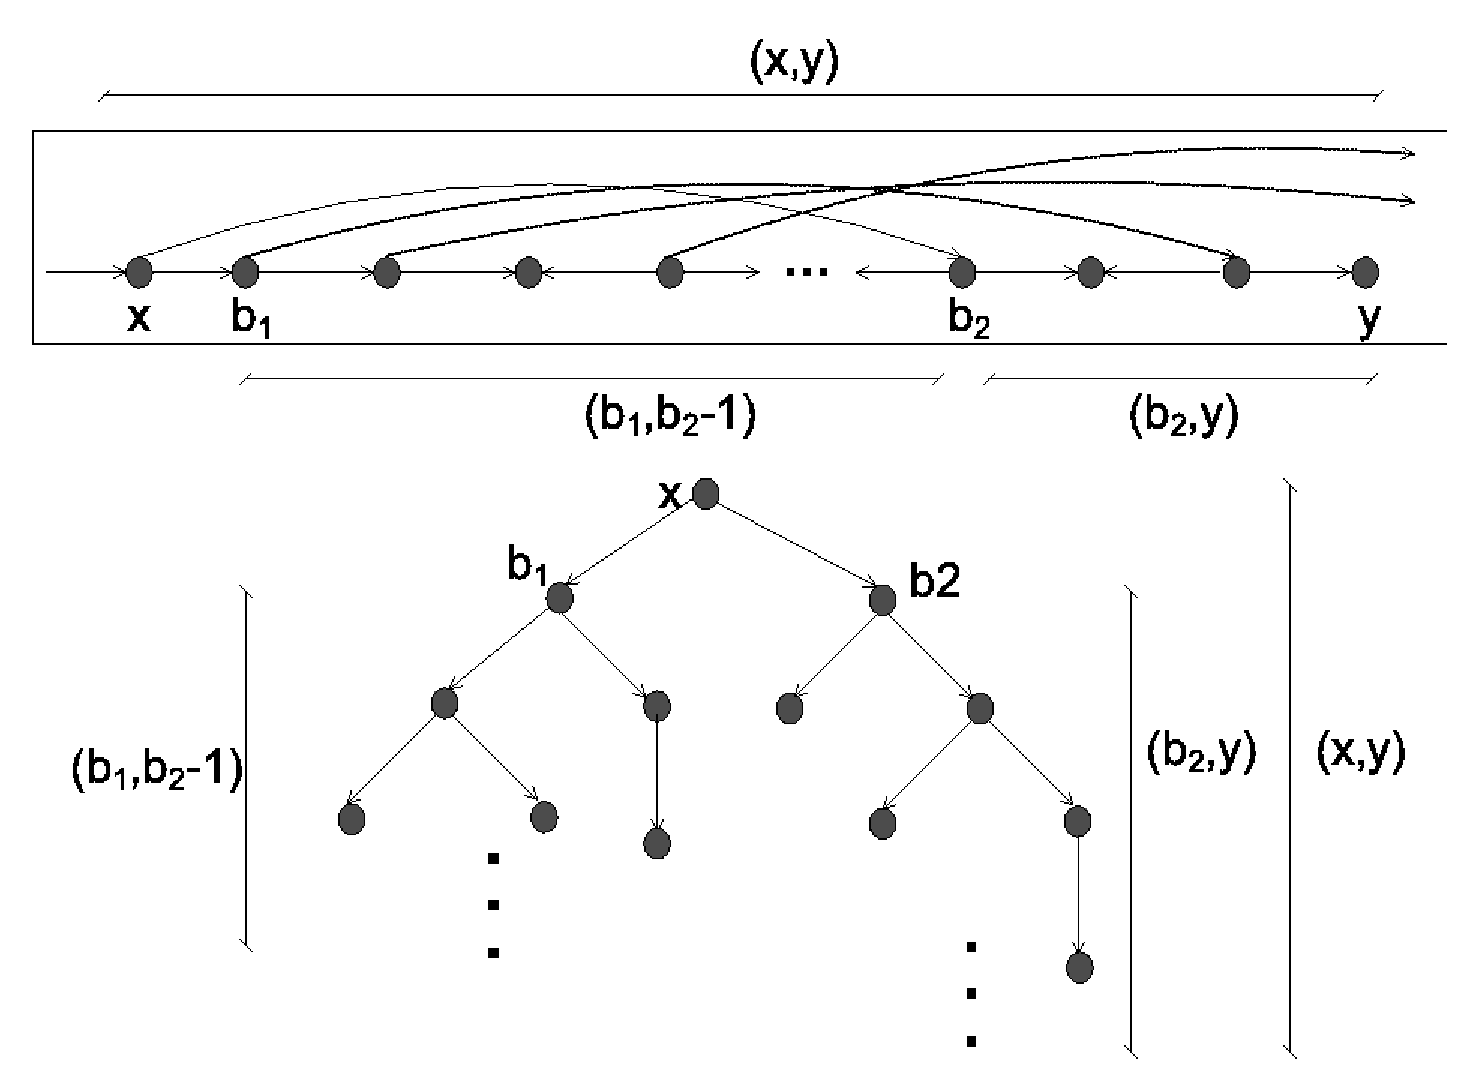
\includegraphics[width=4in]{figs/tree.eps}
\caption[Tree-based overlay broadcast]{Tree-based overlay broadcast}
\label{fig:tree}
\end{figure}  

Broadcast revocation can be used to address the deficiencies of DHT revocation.
As a topic of previous research works~\cite{broadcast, chord_broadcast},
structured overlays can be used without additional state to perform efficient
broadcasts from any point in the overlay to the entire overlay.  In these
papers, analysis and simulations have shown that the approach can be completed
in a network size of $n$ in $O(\log^2 n)$ time with $n$ messages.  The overlay
broadcast algorithm used in this paper provides a complete overlay broadcast in
$O(\log^2 n)$ time with $n$ messages.  When applied to Brunet, as illustrated
in Figure~\ref{fig:tree}, it utilizes the organization of a structured system
with a circular address space that requires peers be connected to those whose
node addresses are the closest to their own, features typical of
one-dimensional structured overlays including Chord~\cite{chord},
Pastry~\cite{pastry}, and Symphony.  Using such an organization, it is possible
to do perform a broadcast with no additional state.  To perform a broadcast,
each node performs the following recursive algorithm:

\begin{algorithmic}
\STATE {\bf BROADCAST(start, end, message)}:
  \STATE RECEIVE(message)
  \FOR{$i$ in length(connections)}
    \STATE n\_start $\gets$ ADDRESS(connections$[i]$)
    \IF {n\_start $\not\in$ $[$start, end$)$}
      \STATE continue
    \ENDIF
    \STATE n\_end $\gets$ ADDRESS(connections$[i+1]$)
    \IF {n\_end $\not\in$ $[$start, end$)$}
      \STATE n\_end $\gets$ end
    \ENDIF
    \STATE msg $\gets$ (BROADCAST, n\_start, n\_end, message)
    \STATE SEND(connections$[i]$, msg)
  \ENDFOR
\end{algorithmic}
with ``connections'' as a circular list of connections in non-decreasing order
from the perspective of the node performing the current recursive, broadcast
step.

In this algorithm, the broadcast initiator uses its own address as the start
and end, thus the broadcast will span the entire overlay after completing
recursive calls at each connected node.  A recursive end, ``n\_end'', must be
inside the region between ``start'' and ``end'', thus if the connection
following the current sending connection, ``connections$[i+1]$'', is not in
that region, it will only broadcast up to ``end'' and not the address specified
by that connection.  To summarize, the overlay is recursively partitioned
amongst the nodes at each hop in the broadcast.  By doing so, all nodes receive
the broadcast without receiving duplicate broadcast messages.

%If you have a single appendix, you need to change {\chapter*{APPENDIX: THIS IS THE FIRST APPENDIX}
%to {\chapter*{APPENDIX: YOUR APPENDIX TITLE HERE} if you have two or more appendices
%you need to change {\chapter{THIS IS THE FIRST APPENDIX}} to
%{\chapter{YOUR APPENDIX TITLE HERE}}
%
%If you make these changes correctly Latex will complain bitterly about the additions to the TOC
%but will make them correctly in a manner acceptable to the Editorial Office.

%\ifthenelse{\value{noa} = 1}
%...................then
%{\chapter*{APPENDIX: EVALUATION TOOLS}
%\label{evaluation_tools}
%\addcontentsline{toc}{chapter}{APPENDIX: EVALUATION TOOLS}
%\chaptermark{Appendix}
%\markboth{Appendix}{Appendix}
%\setcounter{chapter}{1}}
%...................else
{\chapter{EVALUATION TOOLS}
\label{evaluation_tools}}
%...................

Netperf~\cite{netperf} is used to estimate the latency and bandwidth of the
different VN models. The latency is measured by deploying Netperf in the
TCP\_RR mode, which measures the number of 1-byte request-receive transactions
that can be completed in a second. The bandwidth is estimated by running Netperf
in the TCP\_STREAM mode, which is a bulk transfer mode. It should be noted that
in situations where the link bandwidths were asymmetric, Netperf is deployed in
both directions.  Since both latency and bandwidth are dependent on the CPU
comparison, evaluations that include CPU utilization tasks require creating
a baseline first where only Netperf is the only active workload.

SPECjbb~\cite{specjbb} simulates a three-tier web application with all the
clients, the middle tier, and the database running on a single system in a
single address space (inside a JVM). On completion, the benchmark provides the
metric in terms of business of operations per second (bops). The bops score of
the system under test depends on both the CPU and the memory in the system, as
the entire database for the benchmark is held in memory. This benchmark
generates negligible disk activity and no network activity. 



%------------------------------------------%

% Make List of References (BibTeX implemented using the Natbib package)
% un-comment your preferred bibliography style and replace the
% bibliography file "sample" with the name of your .bib file
% REMEMBER!!! If you want un-numbered references comment the Natbib package with
% The numbered options in the packages.tex file and un-comment the package with the authoryear option
% See the included pdfs of the various styles to see the differences.
% The citation style differences are from the \citet{key} and \citep{key} commands
% More options are available; see the Natbib documentation for details


\bibliography{ufsampleETD}
% You can have more than one library of references
%------------------------------------------%

% Bio Sketch %
% Just type your bio in between the brackets
\biography{%

David Isaac Wolinsky was born on October 31, 1982.  He was blessed with an
awesome, Isaac Emmanuel, born November 30, 2009.  Beginning his studies in
August 2001 at the University of Florida, David obtained the following degrees
in electrical and computer engineering: Bachelor of Science in Spring 2005,
Master of Science in Spring 2007, and Doctorate of Philosophy in Summer 2011.
His advisor at the University of Florida was Professor Renato Figueiredo, whom
he began working with since the during the Spring of 2006 at the Advanced
Computing and Information Systems Lab.

His primary research focuses are network virtualization using structured P2P
(peer-to-peer) overlays and grid computing.  The networking research has been
realized in IPOP, a free (BSD - Berkeley Software Distribution licence))
network virtualization software.  Additionally, he has worked on enabling DHTs,
decentralized NAT (network address translation) traversal through relays,
software models for improved network virtualization, and autonomic virtual
networking stacks.  This work is a major contribution to his grid computing
research focus, Grid Appliance, which enables the creation of decentralized,
distributed grids using virtualized, physical, and cloud resources.  Going
forward, he expressed great interested in using these concepts in other
distributed systems such as sensor networks, social networks, cloud services,
or even web services.

During his free time, he enjoys time with my boy, running, playing basketball,
and occasionally playing video games.  At one point, he was ranked in the top
20 on the US East Warcraft III Free For All Ladder.  

}


%------------------------------------------%

\end{document}

%-------------------------------------------------------------------------------------------------------%
